\documentclass{article}
\usepackage{fullpage,booktabs,graphicx,hyperref,float,array}
% generated by grnbench report from result files - do not edit
\newcommand{\gbCiHighAuprcRatioAutoPearsonMotifVsPearsonSigned}{+0.229}
\newcommand{\gbCiHighAuprcRatioBaselinePearsonMotifVsPearsonSigned}{+0.223}
\newcommand{\gbCiHighEprAutoPearsonMotifVsPearsonSigned}{+0.230}
\newcommand{\gbCiHighEprBaselinePearsonMotifVsPearsonSigned}{+0.267}
\newcommand{\gbCiLowAuprcRatioAutoPearsonMotifVsPearsonSigned}{+0.183}
\newcommand{\gbCiLowAuprcRatioBaselinePearsonMotifVsPearsonSigned}{+0.181}
\newcommand{\gbCiLowEprAutoPearsonMotifVsPearsonSigned}{+0.067}
\newcommand{\gbCiLowEprBaselinePearsonMotifVsPearsonSigned}{+0.131}
\newcommand{\gbDiffAuprcRatioAutoPearsonMotifVsPearsonSigned}{+0.206}
\newcommand{\gbDiffAuprcRatioBaselinePearsonMotifVsPearsonSigned}{+0.202}
\newcommand{\gbDiffEprAutoPearsonMotifVsPearsonSigned}{+0.149}
\newcommand{\gbDiffEprBaselinePearsonMotifVsPearsonSigned}{+0.199}
\newcommand{\gbFamilyAuprcRatioAuto}{2}
\newcommand{\gbFamilyAuprcRatioBaseline}{2}
\newcommand{\gbFamilyEprAuto}{2}
\newcommand{\gbFamilyEprBaseline}{2}
\newcommand{\gbMeanAuprcRatioAutoPearsonMotif}{1.579}
\newcommand{\gbMeanAuprcRatioAutoPearsonSigned}{1.373}
\newcommand{\gbNAuprcRatioAutoPearsonMotifVsPearsonSigned}{119}
\newcommand{\gbNAuprcRatioBaselinePearsonMotifVsPearsonSigned}{119}
\newcommand{\gbNAutoPearsonMotif}{119}
\newcommand{\gbNAutoPearsonSigned}{119}
\newcommand{\gbNDatasets}{120}
\newcommand{\gbNEprAutoPearsonMotifVsPearsonSigned}{119}
\newcommand{\gbNEprBaselinePearsonMotifVsPearsonSigned}{119}
\newcommand{\gbPHolmAuprcRatioAutoPearsonMotifVsPearsonSigned}{1.6e-35}
\newcommand{\gbPHolmAuprcRatioBaselinePearsonMotifVsPearsonSigned}{9.2e-38}
\newcommand{\gbPHolmEprAutoPearsonMotifVsPearsonSigned}{0.00042}
\newcommand{\gbPHolmEprBaselinePearsonMotifVsPearsonSigned}{5.3e-08}
\newcommand{\gbPHolmRevAuprcRatioAutoPearsonMotifVsPearsonSigned}{1.000}
\newcommand{\gbPHolmRevAuprcRatioBaselinePearsonMotifVsPearsonSigned}{1.000}
\newcommand{\gbPHolmRevEprAutoPearsonMotifVsPearsonSigned}{1.000}
\newcommand{\gbPHolmRevEprBaselinePearsonMotifVsPearsonSigned}{1.000}

\title{EXP-20261022-GB-1: Confirmatory - does the motif prior lift Pearson's EPR on the 120 confirmatory datasets of the D-057 CELLxGENE pool?}
\author{grnbench report generated from EXP-20261022-GB-1}
\date{}
\begin{document}
\maketitle
\section*{Status}
Experiment EXP-20261022-GB-1, type: confirmatory. Record status: registered. Reproduced by: nobody yet.
\section{Configuration summary}
\begin{table}[H]\centering\small
\caption{Configuration of the run, from the experiment record and the run folder.}
\begin{tabular}{p{0.3\linewidth}p{0.62\linewidth}}\toprule
experiment & EXP-20261022-GB-1 \\
type & confirmatory (pre-registration = the pushed commit that adds this file, before any dataset of the list below is scored) \\
owner & GB (agent-prepared)   issue: \#139 (data: \#141)   registered: 2026-10-22 and LD's reviews of the registration PR: (1) six pool datasets had been scored by EXP-20261001-LD-1; the exclusion now covers benchmarks/results/ and every branch (used\_datasets.py), and the pool was redrawn from the same saved listing (194 datasets kept, those 6 and their studies replaced by 6 others); (2) the scope is the registered pool, not every scRNA-seq dataset, and subgroup breakdowns are declared below; (3) data provenance is an experiment-specific snapshot checked with --require-all; (4) data and large outputs live in a dedicated data folder outside the code checkout; (5) T3 of EXP-20261003-GB-1 is added as a secondary confirmatory family (LM's suggestion). A partial download made on 2026-10-23 under the first version (4.5 GB of exploratory files, nothing scored) is kept; files not in the redrawn pool are deleted before the data check. \\
datasets (rows) & 120 \\
models & pearson\_motif, pearson\_signed \\
arms & auto, baseline \\
code & branch gb/pool-200, synced to a separate cluster checkout \textasciitilde{}/grnbench-pool200 with hpc/hpc.sh sync; the job copies GIT\_COMMIT into the results as CODE\_COMMIT. The commit that runs is the one that adds the data snapshot (below), pushed before any model runs; real\_bench.py and the engine are main's (6917c88), the branch adds only the selection tools and records. \\
code commit (run folder) & 7e4bcb69f1d1c31bc6fbe85820a454cae84ddd68 \\
environment & conda env grnbench on the cluster, Python 3.11, requirements/lock-py311.txt; no extra packages (no torch). \\
machine & Bocconi HPC, partition/QOS stud (1 running + 1 queued job per user), 8 CPUs, 24 h per job. \\
seeds & reference split seed 0 (screen.split\_reference), cell subsample seed 0 (at most 3,000 cells per context, engine\_bench.MAX\_SCORE\_CELLS), scrublet seed 0; regulators = the 150 TFs with most reference targets in the data (MAX\_TFS). The same settings as C4. \\
run folder & EXP-20261022-GB-1 \\
generated & 2026-10-28 18:26 \\
\bottomrule\end{tabular}\end{table}

\section{Methods}
\begin{description}
\item[type] confirmatory (pre-registration = the pushed commit that adds this file, before any dataset of the list below is scored)
\item[hypothesis (h1, primary, directional)] on the datasets of this pool, pearson\_motif (Pearson co-expression rank-producted with the cisTarget motif prior) recovers the top of the CollecTRI evaluation half better than pearson\_signed alone, measured by EPR.
\item[primary endpoint] EPR (early precision ratio: precision in the top k edges, k = reference edges in the scored universe, divided by the reference density; 1 = random) on the CollecTRI evaluation half, **auto** pipeline arm (the engine's screened choice), mean over contexts within a dataset, as computed by real\_bench (metrics.evaluate\_ranking) in C4. Holm: EPR in the baseline arm; AUPRC ratio in the auto arm and in the baseline arm.
\item[unit of analysis] dataset. Planned n = 120; analysed n = datasets with an EPR for both models in the auto arm (printed by the report).
\item[datasets] the 120 datasets of experiments/EXP-20261022-GB-1.datasets.tsv, the confirmatory part of the D-057 pool. How the pool was made, from one saved copy of the CELLxGENE curation listing taken on 2026-10-22 (sha256 e4f05bff6e65c62b6d2c9a077acb2f22b19f80f1bc2c737f52f0520e2ab122bd, kept on the cluster next to the data; not in git): used\_datasets.py scanned experiments/ and benchmarks/results/ on HEAD and the 52 remote branches on 2026-10-23: 71 datasets used before, in 43 studies, all excluded with every dataset of those studies. The pool (experiments/EXP-20261022-GB.pool.tsv) is the first 200 of the selector's round-robin over assay x organism (smallest files first) out of 202 eligible studies; 200 datasets from 200 studies. The split is by sha256 of seed and dataset id, fixed before any score. The 120: 65.5 GB, 25 files above 1 GB, 18 assays.
\item[exclusion rules (fixed now)] (a) a dataset whose download fails or whose sha256 cannot be recorded is reported as missing and replaced by nobody; (b) a dataset refused at ingest as not raw counts (D-001) is reported and not scored; (c) datasets with fewer than 50 reference edges among their genes are not scored (MIN\_REFERENCE\_EDGES); (d) a dataset where a model errors is dropped from the pair and reported; (e) a dataset still unfinished after the job and one resubmission of the same commit (TIMEOUT or out of memory; the resubmission may use fewer workers or more memory) is reported as missing, with its size; (f) no other exclusion, no outlier removal.
\item[comparison family] models run = \{pearson\_signed, pearson\_motif\}, so real\_bench.DECLARED\_PAIRS restricted to them is the single pair (pearson\_motif, pearson\_signed); both directions = 2 directed hypotheses per metric and arm. H1 is the EPR / auto family.
\item[test] paired t over datasets via compare\_units (95\% interval of the mean paired difference, a one-sided p in each direction), Holm over the 2 directed hypotheses of the EPR / auto family, alpha 0.05, as printed by real\_bench.py report. **H1 is supported** if p\_Holm(pearson\_motif > pearson\_signed) < 0.05; **refuted** if p\_Holm(pearson\_signed > pearson\_motif) < 0.05; otherwise inconclusive (not evidence of equality).
\item[seeds] reference split seed 0 (screen.split\_reference), cell subsample seed 0 (at most 3,000 cells per context, engine\_bench.MAX\_SCORE\_CELLS), scrublet seed 0; regulators = the 150 TFs with most reference targets in the data (MAX\_TFS). The same settings as C4.
\item[code] branch gb/pool-200, synced to a separate cluster checkout \textasciitilde{}/grnbench-pool200 with hpc/hpc.sh sync; the job copies GIT\_COMMIT into the results as CODE\_COMMIT. The commit that runs is the one that adds the data snapshot (below), pushed before any model runs; real\_bench.py and the engine are main's (6917c88), the branch adds only the selection tools and records.
\item[environment] conda env grnbench on the cluster, Python 3.11, requirements/lock-py311.txt; no extra packages (no torch).
\item[machine] Bocconi HPC, partition/QOS stud (1 running + 1 queued job per user), 8 CPUs, 24 h per job.
\item[models scored] pearson\_motif, pearson\_signed
\end{description}

\section{Results}
\subsection{Primary comparison}
\paragraph{Pre-registered primary hypothesis.} pearson\_motif $>$ pearson\_signed on EPR, auto pipeline. Mean paired difference \gbDiffEprAutoPearsonMotifVsPearsonSigned{} (95\% interval \gbCiLowEprAutoPearsonMotifVsPearsonSigned{} to \gbCiHighEprAutoPearsonMotifVsPearsonSigned{}), n = \gbNEprAutoPearsonMotifVsPearsonSigned{} datasets, paired t, Holm over \gbFamilyEprAuto{} directed hypotheses: $p_{\mathrm{Holm}}$ = \gbPHolmEprAutoPearsonMotifVsPearsonSigned{}. Verdict by the rule fixed in the record: \textbf{supported}.

\subsection{Performance per model, across datasets}
\begin{table}[H]\centering\small
\caption{Reference recovery per model (CollecTRI evaluation half; AUPRC ratio, 1 = random). Unit = dataset; n per model shown.}
\begin{tabular}{lrrrr}\toprule
model & n & mean (auto) & median (auto) & mean (baseline) \\ \midrule
pearson\_motif & 119 & 1.579 & 1.550 & 1.514 \\
pearson\_signed & 119 & 1.373 & 1.349 & 1.313 \\
\bottomrule\end{tabular}\end{table}

\subsection{Performance per dataset}
\begin{table}[H]\centering\scriptsize
\caption{AUPRC ratio per dataset, auto pipeline (1 = random); the unit of analysis.}
\resizebox{\linewidth}{!}{\begin{tabular}{lrr}\toprule
dataset & pearson\_motif & pearson\_signed \\ \midrule
10x-3-v2\_\_homo-sapiens\_\_anterior-wall-of-left-ve & 1.31 & 1.24 \\
10x-3-v2\_\_homo-sapiens\_\_blood\_\_ae5341b8 & 1.72 & 1.54 \\
10x-3-v2\_\_homo-sapiens\_\_brain\_\_dc30c3ec & 1.29 & 1.11 \\
10x-3-v2\_\_homo-sapiens\_\_breast\_\_9a64bf99 & 1.58 & 1.49 \\
10x-3-v2\_\_homo-sapiens\_\_caudate-lobe-of-liver\_\_a & 1.49 & 1.27 \\
10x-3-v2\_\_homo-sapiens\_\_cortex-of-kidney\_\_105c7d & 1.95 & 1.78 \\
10x-3-v2\_\_homo-sapiens\_\_dental-pulp\_\_bdd109f1 & 2.24 & 1.98 \\
10x-3-v2\_\_homo-sapiens\_\_epithelium-of-rectum\_\_80 & 1.45 & 1.22 \\
10x-3-v2\_\_homo-sapiens\_\_fovea-centralis\_\_babbf9f & 1.42 & 1.15 \\
10x-3-v2\_\_homo-sapiens\_\_kidney\_\_8dc29642 & 1.61 & 1.55 \\
10x-3-v2\_\_homo-sapiens\_\_lung\_\_6e00ccf7 & 1.51 & 1.23 \\
10x-3-v2\_\_homo-sapiens\_\_mammary-gland-connective & 2.18 & 1.85 \\
10x-3-v2\_\_homo-sapiens\_\_ovary\_\_1f1c5c14 & 1.55 & 1.45 \\
10x-3-v2\_\_homo-sapiens\_\_respiratory-airway\_\_8fcf & 1.20 & 1.00 \\
10x-3-v2\_\_homo-sapiens\_\_skin-of-prepuce-of-penis & 1.49 & 1.40 \\
10x-3-v2\_\_homo-sapiens\_\_thymus\_\_11ff73e8 & 1.65 & 1.50 \\
10x-3-v2\_\_homo-sapiens\_\_zone-of-skin\_\_124744b8 & 1.53 & 1.41 \\
10x-3-v2\_\_mus-musculus\_\_hindlimb-muscle\_\_bedee31 & 1.62 & 1.61 \\
10x-3-v3\_\_homo-sapiens\_\_abdomen\_\_7b95971d & 1.22 & 1.15 \\
10x-3-v3\_\_homo-sapiens\_\_abdomen\_\_97d9238c & 1.50 & 1.37 \\
10x-3-v3\_\_homo-sapiens\_\_apex-of-heart\_\_2e9d2f32 & 1.47 & 1.39 \\
10x-3-v3\_\_homo-sapiens\_\_blood\_\_19e46756 & 1.82 & 1.65 \\
10x-3-v3\_\_homo-sapiens\_\_blood\_\_20fae564 & 1.50 & 1.35 \\
10x-3-v3\_\_homo-sapiens\_\_blood\_\_738942eb & 1.85 & 1.42 \\
10x-3-v3\_\_homo-sapiens\_\_blood\_\_a199ca73 & 1.91 & 1.69 \\
10x-3-v3\_\_homo-sapiens\_\_blood\_\_d9f3a82c & 1.47 & 1.22 \\
10x-3-v3\_\_homo-sapiens\_\_blood\_\_de2c780c & 1.73 & 1.65 \\
10x-3-v3\_\_homo-sapiens\_\_bone-marrow\_\_343ff97c & 1.74 & 1.56 \\
10x-3-v3\_\_homo-sapiens\_\_breast\_\_24ec2dc5 & 1.58 & 1.39 \\
10x-3-v3\_\_homo-sapiens\_\_brodmann-1909-area-13\_\_f & 1.30 & 1.02 \\
10x-3-v3\_\_homo-sapiens\_\_brodmann-1909-area-4\_\_c8 & 1.28 & 1.03 \\
10x-3-v3\_\_homo-sapiens\_\_brown-preadipocyte\_\_137c & 1.33 & 1.17 \\
10x-3-v3\_\_homo-sapiens\_\_calcaneal-tendon\_\_ef0fc6 & 1.81 & 1.44 \\
10x-3-v3\_\_homo-sapiens\_\_calcaneal-tendon\_\_f641d6 & 1.63 & 1.24 \\
10x-3-v3\_\_homo-sapiens\_\_caudate-nucleus\_\_c893ddc & 1.59 & 1.35 \\
10x-3-v3\_\_homo-sapiens\_\_cerebellum\_\_be884a28 & 1.50 & 1.26 \\
10x-3-v3\_\_homo-sapiens\_\_cornea\_\_8058d760 & 1.44 & 1.19 \\
10x-3-v3\_\_homo-sapiens\_\_cortex-of-kidney\_\_07854d & 1.46 & 1.30 \\
10x-3-v3\_\_homo-sapiens\_\_cortex-of-kidney\_\_0bae7e & 1.57 & 1.38 \\
10x-3-v3\_\_homo-sapiens\_\_cranial-nerve-ii\_\_374edd & 1.48 & 1.33 \\
10x-3-v3\_\_homo-sapiens\_\_cranial-nerve-ii\_\_9f1a89 & 1.43 & 1.20 \\
10x-3-v3\_\_homo-sapiens\_\_dome-of-urinary-bladder\_ & 1.41 & 1.22 \\
10x-3-v3\_\_homo-sapiens\_\_endometrium\_\_76150f40 & 1.70 & 1.46 \\
10x-3-v3\_\_homo-sapiens\_\_endometrium\_\_7a419302 & 1.63 & 1.48 \\
10x-3-v3\_\_homo-sapiens\_\_entorhinal-cortex\_\_24584 & 1.36 & 1.08 \\
10x-3-v3\_\_homo-sapiens\_\_fallopian-tube\_\_30f5e171 & 1.97 & 2.09 \\
10x-3-v3\_\_homo-sapiens\_\_fovea-centralis\_\_11ef37e & 1.51 & 1.15 \\
10x-3-v3\_\_homo-sapiens\_\_fovea-centralis\_\_af8b241 & 2.01 & 1.96 \\
10x-3-v3\_\_homo-sapiens\_\_fovea-centralis\_\_e404d41 & 1.51 & 1.08 \\
10x-3-v3\_\_homo-sapiens\_\_fovea-centralis\_\_f5be9ed & 1.61 & 1.50 \\
10x-3-v3\_\_homo-sapiens\_\_heart-left-ventricle\_\_f1 & 1.37 & 1.25 \\
10x-3-v3\_\_homo-sapiens\_\_kidney\_\_ea01c125 & 1.74 & 1.70 \\
10x-3-v3\_\_homo-sapiens\_\_left-atrium-auricular-re & 1.73 & 1.67 \\
10x-3-v3\_\_homo-sapiens\_\_lens-of-camera-type-eye\_ & 1.45 & 1.02 \\
10x-3-v3\_\_homo-sapiens\_\_liver\_\_0bbf93aa & 1.80 & 1.44 \\
10x-3-v3\_\_homo-sapiens\_\_liver\_\_ec6ceff8 & 1.32 & 1.29 \\
10x-3-v3\_\_homo-sapiens\_\_lung-parenchyma\_\_01ff5cf & 1.45 & 1.35 \\
10x-3-v3\_\_homo-sapiens\_\_lung-parenchyma\_\_8fbed30 & 1.68 & 1.50 \\
10x-3-v3\_\_homo-sapiens\_\_lung\_\_6ba45a2b & 2.21 & 1.43 \\
10x-3-v3\_\_homo-sapiens\_\_lung\_\_d8da613f & 1.42 & 1.21 \\
10x-3-v3\_\_homo-sapiens\_\_mesenteric-artery\_\_42b6a & 1.74 & 1.61 \\
10x-3-v3\_\_homo-sapiens\_\_minor-salivary-gland\_\_9a & 1.81 & 1.63 \\
10x-3-v3\_\_homo-sapiens\_\_neocortex\_\_3a8aec06 & 1.90 & 1.58 \\
10x-3-v3\_\_homo-sapiens\_\_neocortex\_\_4859642c & 1.39 & 1.25 \\
10x-3-v3\_\_homo-sapiens\_\_occipital-cortex\_\_e63612 & 1.55 & 1.31 \\
10x-3-v3\_\_homo-sapiens\_\_oropharynx\_\_b6b5ea88 & 1.91 & 1.83 \\
10x-3-v3\_\_homo-sapiens\_\_ovary\_\_3a702020 & 1.33 & 1.19 \\
10x-3-v3\_\_homo-sapiens\_\_ovary\_\_a9bedd04 & 1.35 & 1.23 \\
10x-3-v3\_\_homo-sapiens\_\_placenta\_\_b7efc0ba & 1.69 & 1.44 \\
10x-3-v3\_\_homo-sapiens\_\_prefrontal-cortex\_\_fe2ee & 1.54 & 1.27 \\
10x-3-v3\_\_homo-sapiens\_\_right-atrium-auricular-r & 1.61 & 1.41 \\
10x-3-v3\_\_homo-sapiens\_\_right-temporal-lobe\_\_145 & 2.01 & 1.59 \\
10x-3-v3\_\_homo-sapiens\_\_skin-of-body\_\_b796f27e & 1.71 & 1.56 \\
10x-3-v3\_\_homo-sapiens\_\_tendon-of-semitendinosus & 1.45 & 1.13 \\
10x-3-v3\_\_homo-sapiens\_\_upper-lobe-of-left-lung\_ & 1.86 & 1.81 \\
10x-3-v3\_\_homo-sapiens\_\_visceral-fat\_\_1405dd3e & 1.74 & 1.39 \\
10x-3-v3\_\_mus-musculus\_\_aorta\_\_f7417545 & 1.42 & 1.36 \\
10x-3-v3\_\_mus-musculus\_\_brain-gray-matter\_\_6347c & 1.40 & 1.23 \\
10x-3-v3\_\_mus-musculus\_\_brain\_\_e056b20b & 1.72 & 1.69 \\
10x-3-v3\_\_mus-musculus\_\_cerebral-cortex\_\_0e1c706 & 1.55 & 1.21 \\
10x-3-v3\_\_mus-musculus\_\_cerebral-cortex\_\_1299021 & 1.10 & 1.00 \\
10x-3-v3\_\_mus-musculus\_\_gastrocnemius\_\_2ab892f9 & 1.18 & 1.06 \\
10x-3-v3\_\_mus-musculus\_\_gingiva\_\_e04cb7d9 & 1.54 & 1.47 \\
10x-3-v3\_\_mus-musculus\_\_liver\_\_e9de826e & 1.34 & 1.25 \\
10x-3-v3\_\_mus-musculus\_\_middle-lobe-of-right-lun & 1.67 & 1.40 \\
10x-3-v3\_\_mus-musculus\_\_ovary\_\_55d66f2a & 1.57 & 1.37 \\
10x-3-v3\_\_mus-musculus\_\_tracheal-epithelial-cell & 1.42 & 1.32 \\
10x-5-transcription-profiling\_\_homo-sapiens\_\_adr & 1.66 & 1.35 \\
10x-5-transcription-profiling\_\_homo-sapiens\_\_lun & 1.87 & 1.60 \\
10x-5-v1\_\_homo-sapiens\_\_blood\_\_5b25a46f & 1.81 & 1.42 \\
10x-5-v1\_\_homo-sapiens\_\_blood\_\_c2a461b1 & 1.93 & 1.51 \\
10x-5-v1\_\_homo-sapiens\_\_blood\_\_fa8605cf & 1.89 & 1.45 \\
10x-5-v1\_\_homo-sapiens\_\_bone-marrow\_\_965386e9 & n/a & n/a \\
10x-5-v1\_\_homo-sapiens\_\_lymph-node\_\_99950e99 & 1.54 & 1.30 \\
10x-5-v1\_\_homo-sapiens\_\_t-cell\_\_0c774045 & 1.64 & 1.31 \\
10x-5-v1\_\_homo-sapiens\_\_t-cell\_\_460dfe21 & 1.63 & 1.23 \\
10x-5-v1\_\_homo-sapiens\_\_thymus\_\_8d73847b & 1.44 & 1.15 \\
10x-5-v1\_\_mus-musculus\_\_gonad\_\_a13bda79 & 1.48 & 1.40 \\
10x-5-v2\_\_homo-sapiens\_\_blood\_\_30c2a6fd & 1.61 & 1.28 \\
10x-5-v2\_\_homo-sapiens\_\_blood\_\_bd65a70f & 1.60 & 1.48 \\
10x-multiome\_\_homo-sapiens\_\_amygdala\_\_835fa5c4 & 1.44 & 1.27 \\
10x-multiome\_\_homo-sapiens\_\_anterior-cingulate-c & 1.40 & 1.16 \\
10x-multiome\_\_homo-sapiens\_\_frontal-lobe\_\_01b847 & 1.44 & 1.23 \\
10x-multiome\_\_homo-sapiens\_\_kidney\_\_867757c1 & 1.35 & 1.16 \\
10x-multiome\_\_homo-sapiens\_\_retina\_\_322c816f & 1.28 & 1.10 \\
10x-multiome\_\_mus-musculus\_\_kidney\_\_25818bf7 & 1.29 & 1.10 \\
10x-next-gem-flex-v1\_\_homo-sapiens\_\_endometrium\_ & 1.46 & 1.47 \\
10x-next-gem-flex-v1\_\_homo-sapiens\_\_parenchyma-o & 1.56 & 1.50 \\
asteria-scrna-seq-kit\_\_homo-sapiens\_\_blood\_\_27d3 & 1.68 & 1.29 \\
bd-rhapsody-whole-transcriptome-analysis\_\_homo-s & 1.65 & 1.53 \\
mars-seq\_\_homo-sapiens\_\_bone-marrow\_\_e22482ee & 1.60 & 1.33 \\
mct-seq\_\_homo-sapiens\_\_brodmann-1909-area-46\_\_43 & 1.61 & 1.11 \\
sci-plex\_\_homo-sapiens\_\_k-562\_\_38a78e91 & 1.44 & 1.19 \\
seq-well-s3\_\_homo-sapiens\_\_nasopharynx\_\_13b61a7d & 2.33 & 2.14 \\
seq-well\_\_homo-sapiens\_\_blood\_\_456e8b9b & 1.56 & 1.32 \\
smart-seq-v4\_\_mus-musculus\_\_primary-motor-cortex & 1.22 & 1.03 \\
smart-seq2\_\_homo-sapiens\_\_blood\_\_e04daea4 & 1.67 & 1.51 \\
smart-seq2\_\_homo-sapiens\_\_heart-left-ventricle\_\_ & 1.37 & 1.21 \\
smart-seq\_\_mus-musculus\_\_primary-visual-cortex\_\_ & 1.32 & 1.06 \\
split-seq\_\_homo-sapiens\_\_cerebellum\_\_b2dda353 & 1.32 & 1.14 \\
\midrule
mean & 1.58 & 1.37 \\
median & 1.55 & 1.35 \\
SD & 0.23 & 0.23 \\
\bottomrule\end{tabular}}\end{table}

\subsection{Comparative summary: declared comparisons}
\begin{table}[H]\centering\small
\caption{Declared comparisons, AUPRC ratio, auto pipeline: paired t over datasets (compare\_units), one-sided p per direction, Holm over 2 directed hypotheses; 95\% interval of the mean paired difference.}
\begin{tabular}{llrrlrrl}\toprule
A & B & n & mean A$-$B & 95\% interval & $p_{A>B}$ Holm & $p_{B>A}$ Holm & supported \\ \midrule
pearson\_motif & pearson\_signed & 119 & +0.206 & [+0.183, +0.229] & 1.6e-35 & 1.000 & pearson\_motif \\
\bottomrule\end{tabular}\end{table}

\begin{table}[H]\centering\small
\caption{Declared comparisons, AUPRC ratio, baseline pipeline: paired t over datasets (compare\_units), one-sided p per direction, Holm over 2 directed hypotheses; 95\% interval of the mean paired difference.}
\begin{tabular}{llrrlrrl}\toprule
A & B & n & mean A$-$B & 95\% interval & $p_{A>B}$ Holm & $p_{B>A}$ Holm & supported \\ \midrule
pearson\_motif & pearson\_signed & 119 & +0.202 & [+0.181, +0.223] & 9.2e-38 & 1.000 & pearson\_motif \\
\bottomrule\end{tabular}\end{table}

\begin{table}[H]\centering\small
\caption{Declared comparisons, EPR, auto pipeline: paired t over datasets (compare\_units), one-sided p per direction, Holm over 2 directed hypotheses; 95\% interval of the mean paired difference.}
\begin{tabular}{llrrlrrl}\toprule
A & B & n & mean A$-$B & 95\% interval & $p_{A>B}$ Holm & $p_{B>A}$ Holm & supported \\ \midrule
pearson\_motif & pearson\_signed & 119 & +0.149 & [+0.067, +0.230] & 0.00042 & 1.000 & pearson\_motif \\
\bottomrule\end{tabular}\end{table}

\begin{table}[H]\centering\small
\caption{Declared comparisons, EPR, baseline pipeline: paired t over datasets (compare\_units), one-sided p per direction, Holm over 2 directed hypotheses; 95\% interval of the mean paired difference.}
\begin{tabular}{llrrlrrl}\toprule
A & B & n & mean A$-$B & 95\% interval & $p_{A>B}$ Holm & $p_{B>A}$ Holm & supported \\ \midrule
pearson\_motif & pearson\_signed & 119 & +0.199 & [+0.131, +0.267] & 5.3e-08 & 1.000 & pearson\_motif \\
\bottomrule\end{tabular}\end{table}

\section{Visualizations and explainability}
\begin{figure}[H]\centering
\includegraphics[width=0.85\linewidth]{../viz/calibration_cxg__10x-3-v2__homo-sapiens__anterior-wall-of-left-ventricl__4ed927e9.png}
\caption{-   (n = 20000 edges) - built from  pearson\_motif.tsv.gz}
\end{figure}
\begin{figure}[H]\centering
\includegraphics[width=0.85\linewidth]{../viz/calibration_cxg__10x-3-v2__homo-sapiens__blood__ae5341b8.png}
\caption{-   (n = 20000 edges) - built from  pearson\_motif.tsv.gz}
\end{figure}
\begin{figure}[H]\centering
\includegraphics[width=0.85\linewidth]{../viz/calibration_cxg__10x-3-v2__homo-sapiens__brain__dc30c3ec.png}
\caption{-   (n = 20000 edges) - built from  pearson\_motif.tsv.gz}
\end{figure}
\begin{figure}[H]\centering
\includegraphics[width=0.85\linewidth]{../viz/calibration_cxg__10x-3-v2__homo-sapiens__breast__9a64bf99.png}
\caption{-   (n = 20000 edges) - built from  pearson\_motif.tsv.gz}
\end{figure}
\begin{figure}[H]\centering
\includegraphics[width=0.85\linewidth]{../viz/calibration_cxg__10x-3-v2__homo-sapiens__caudate-lobe-of-liver__a43aa46b.png}
\caption{-   (n = 20000 edges) - built from  pearson\_motif.tsv.gz}
\end{figure}
\begin{figure}[H]\centering
\includegraphics[width=0.85\linewidth]{../viz/calibration_cxg__10x-3-v2__homo-sapiens__cortex-of-kidney__105c7dad.png}
\caption{-   (n = 20000 edges) - built from  pearson\_motif.tsv.gz}
\end{figure}
\begin{figure}[H]\centering
\includegraphics[width=0.85\linewidth]{../viz/calibration_cxg__10x-3-v2__homo-sapiens__dental-pulp__bdd109f1.png}
\caption{-   (n = 20000 edges) - built from  pearson\_motif.tsv.gz}
\end{figure}
\begin{figure}[H]\centering
\includegraphics[width=0.85\linewidth]{../viz/calibration_cxg__10x-3-v2__homo-sapiens__epithelium-of-rectum__80d7111d.png}
\caption{-   (n = 20000 edges) - built from  pearson\_motif.tsv.gz}
\end{figure}
\begin{figure}[H]\centering
\includegraphics[width=0.85\linewidth]{../viz/calibration_cxg__10x-3-v2__homo-sapiens__fovea-centralis__babbf9f3.png}
\caption{-   (n = 20000 edges) - built from  pearson\_motif.tsv.gz}
\end{figure}
\begin{figure}[H]\centering
\includegraphics[width=0.85\linewidth]{../viz/calibration_cxg__10x-3-v2__homo-sapiens__kidney__8dc29642.png}
\caption{-   (n = 20000 edges) - built from  pearson\_motif.tsv.gz}
\end{figure}
\begin{figure}[H]\centering
\includegraphics[width=0.85\linewidth]{../viz/calibration_cxg__10x-3-v2__homo-sapiens__lung__6e00ccf7.png}
\caption{-   (n = 20000 edges) - built from  pearson\_motif.tsv.gz}
\end{figure}
\begin{figure}[H]\centering
\includegraphics[width=0.85\linewidth]{../viz/calibration_cxg__10x-3-v2__homo-sapiens__mammary-gland-connective-tissu__68b6114f.png}
\caption{-   (n = 20000 edges) - built from  pearson\_motif.tsv.gz}
\end{figure}
\begin{figure}[H]\centering
\includegraphics[width=0.85\linewidth]{../viz/calibration_cxg__10x-3-v2__homo-sapiens__ovary__1f1c5c14.png}
\caption{-   (n = 20000 edges) - built from  pearson\_motif.tsv.gz}
\end{figure}
\begin{figure}[H]\centering
\includegraphics[width=0.85\linewidth]{../viz/calibration_cxg__10x-3-v2__homo-sapiens__respiratory-airway__8fcf0ccc.png}
\caption{-   (n = 20000 edges) - built from  pearson\_motif.tsv.gz}
\end{figure}
\begin{figure}[H]\centering
\includegraphics[width=0.85\linewidth]{../viz/calibration_cxg__10x-3-v2__homo-sapiens__skin-of-prepuce-of-penis__f512b8b6.png}
\caption{-   (n = 20000 edges) - built from  pearson\_motif.tsv.gz}
\end{figure}
\begin{figure}[H]\centering
\includegraphics[width=0.85\linewidth]{../viz/calibration_cxg__10x-3-v2__homo-sapiens__thymus__11ff73e8.png}
\caption{-   (n = 20000 edges) - built from  pearson\_motif.tsv.gz}
\end{figure}
\begin{figure}[H]\centering
\includegraphics[width=0.85\linewidth]{../viz/calibration_cxg__10x-3-v2__homo-sapiens__zone-of-skin__124744b8.png}
\caption{-   (n = 20000 edges) - built from  pearson\_motif.tsv.gz}
\end{figure}
\begin{figure}[H]\centering
\includegraphics[width=0.85\linewidth]{../viz/calibration_cxg__10x-3-v2__mus-musculus__hindlimb-muscle__bedee313.png}
\caption{-   (n = 20000 edges) - built from  pearson\_motif.tsv.gz}
\end{figure}
\begin{figure}[H]\centering
\includegraphics[width=0.85\linewidth]{../viz/calibration_cxg__10x-3-v3__homo-sapiens__abdomen__7b95971d.png}
\caption{-   (n = 20000 edges) - built from  pearson\_motif.tsv.gz}
\end{figure}
\begin{figure}[H]\centering
\includegraphics[width=0.85\linewidth]{../viz/calibration_cxg__10x-3-v3__homo-sapiens__abdomen__97d9238c.png}
\caption{-   (n = 20000 edges) - built from  pearson\_motif.tsv.gz}
\end{figure}
\begin{figure}[H]\centering
\includegraphics[width=0.85\linewidth]{../viz/calibration_cxg__10x-3-v3__homo-sapiens__apex-of-heart__2e9d2f32.png}
\caption{-   (n = 20000 edges) - built from  pearson\_motif.tsv.gz}
\end{figure}
\begin{figure}[H]\centering
\includegraphics[width=0.85\linewidth]{../viz/calibration_cxg__10x-3-v3__homo-sapiens__blood__19e46756.png}
\caption{-   (n = 20000 edges) - built from  pearson\_motif.tsv.gz}
\end{figure}
\begin{figure}[H]\centering
\includegraphics[width=0.85\linewidth]{../viz/calibration_cxg__10x-3-v3__homo-sapiens__blood__20fae564.png}
\caption{-   (n = 20000 edges) - built from  pearson\_motif.tsv.gz}
\end{figure}
\begin{figure}[H]\centering
\includegraphics[width=0.85\linewidth]{../viz/calibration_cxg__10x-3-v3__homo-sapiens__blood__738942eb.png}
\caption{-   (n = 20000 edges) - built from  pearson\_motif.tsv.gz}
\end{figure}
\begin{figure}[H]\centering
\includegraphics[width=0.85\linewidth]{../viz/calibration_cxg__10x-3-v3__homo-sapiens__blood__a199ca73.png}
\caption{-   (n = 20000 edges) - built from  pearson\_motif.tsv.gz}
\end{figure}
\begin{figure}[H]\centering
\includegraphics[width=0.85\linewidth]{../viz/calibration_cxg__10x-3-v3__homo-sapiens__blood__d9f3a82c.png}
\caption{-   (n = 20000 edges) - built from  pearson\_motif.tsv.gz}
\end{figure}
\begin{figure}[H]\centering
\includegraphics[width=0.85\linewidth]{../viz/calibration_cxg__10x-3-v3__homo-sapiens__blood__de2c780c.png}
\caption{-   (n = 20000 edges) - built from  pearson\_motif.tsv.gz}
\end{figure}
\begin{figure}[H]\centering
\includegraphics[width=0.85\linewidth]{../viz/calibration_cxg__10x-3-v3__homo-sapiens__bone-marrow__343ff97c.png}
\caption{-   (n = 20000 edges) - built from  pearson\_motif.tsv.gz}
\end{figure}
\begin{figure}[H]\centering
\includegraphics[width=0.85\linewidth]{../viz/calibration_cxg__10x-3-v3__homo-sapiens__breast__24ec2dc5.png}
\caption{-   (n = 20000 edges) - built from  pearson\_motif.tsv.gz}
\end{figure}
\begin{figure}[H]\centering
\includegraphics[width=0.85\linewidth]{../viz/calibration_cxg__10x-3-v3__homo-sapiens__brodmann-1909-area-13__f16f4108.png}
\caption{-   (n = 20000 edges) - built from  pearson\_motif.tsv.gz}
\end{figure}
\begin{figure}[H]\centering
\includegraphics[width=0.85\linewidth]{../viz/calibration_cxg__10x-3-v3__homo-sapiens__brodmann-1909-area-4__c8f83821.png}
\caption{-   (n = 20000 edges) - built from  pearson\_motif.tsv.gz}
\end{figure}
\begin{figure}[H]\centering
\includegraphics[width=0.85\linewidth]{../viz/calibration_cxg__10x-3-v3__homo-sapiens__brown-preadipocyte__137ca42b.png}
\caption{-   (n = 20000 edges) - built from  pearson\_motif.tsv.gz}
\end{figure}
\begin{figure}[H]\centering
\includegraphics[width=0.85\linewidth]{../viz/calibration_cxg__10x-3-v3__homo-sapiens__calcaneal-tendon__ef0fc6ac.png}
\caption{-   (n = 20000 edges) - built from  pearson\_motif.tsv.gz}
\end{figure}
\begin{figure}[H]\centering
\includegraphics[width=0.85\linewidth]{../viz/calibration_cxg__10x-3-v3__homo-sapiens__calcaneal-tendon__f641d68a.png}
\caption{-   (n = 20000 edges) - built from  pearson\_motif.tsv.gz}
\end{figure}
\begin{figure}[H]\centering
\includegraphics[width=0.85\linewidth]{../viz/calibration_cxg__10x-3-v3__homo-sapiens__caudate-nucleus__c893ddc3.png}
\caption{-   (n = 20000 edges) - built from  pearson\_motif.tsv.gz}
\end{figure}
\begin{figure}[H]\centering
\includegraphics[width=0.85\linewidth]{../viz/calibration_cxg__10x-3-v3__homo-sapiens__cerebellum__be884a28.png}
\caption{-   (n = 20000 edges) - built from  pearson\_motif.tsv.gz}
\end{figure}
\begin{figure}[H]\centering
\includegraphics[width=0.85\linewidth]{../viz/calibration_cxg__10x-3-v3__homo-sapiens__cornea__8058d760.png}
\caption{-   (n = 20000 edges) - built from  pearson\_motif.tsv.gz}
\end{figure}
\begin{figure}[H]\centering
\includegraphics[width=0.85\linewidth]{../viz/calibration_cxg__10x-3-v3__homo-sapiens__cortex-of-kidney__07854d9c.png}
\caption{-   (n = 20000 edges) - built from  pearson\_motif.tsv.gz}
\end{figure}
\begin{figure}[H]\centering
\includegraphics[width=0.85\linewidth]{../viz/calibration_cxg__10x-3-v3__homo-sapiens__cortex-of-kidney__0bae7ebf.png}
\caption{-   (n = 20000 edges) - built from  pearson\_motif.tsv.gz}
\end{figure}
\begin{figure}[H]\centering
\includegraphics[width=0.85\linewidth]{../viz/calibration_cxg__10x-3-v3__homo-sapiens__cranial-nerve-ii__374edd6c.png}
\caption{-   (n = 20000 edges) - built from  pearson\_motif.tsv.gz}
\end{figure}
\begin{figure}[H]\centering
\includegraphics[width=0.85\linewidth]{../viz/calibration_cxg__10x-3-v3__homo-sapiens__cranial-nerve-ii__9f1a899f.png}
\caption{-   (n = 20000 edges) - built from  pearson\_motif.tsv.gz}
\end{figure}
\begin{figure}[H]\centering
\includegraphics[width=0.85\linewidth]{../viz/calibration_cxg__10x-3-v3__homo-sapiens__dome-of-urinary-bladder__601c7454.png}
\caption{-   (n = 20000 edges) - built from  pearson\_motif.tsv.gz}
\end{figure}
\begin{figure}[H]\centering
\includegraphics[width=0.85\linewidth]{../viz/calibration_cxg__10x-3-v3__homo-sapiens__endometrium__76150f40.png}
\caption{-   (n = 20000 edges) - built from  pearson\_motif.tsv.gz}
\end{figure}
\begin{figure}[H]\centering
\includegraphics[width=0.85\linewidth]{../viz/calibration_cxg__10x-3-v3__homo-sapiens__endometrium__7a419302.png}
\caption{-   (n = 20000 edges) - built from  pearson\_motif.tsv.gz}
\end{figure}
\begin{figure}[H]\centering
\includegraphics[width=0.85\linewidth]{../viz/calibration_cxg__10x-3-v3__homo-sapiens__entorhinal-cortex__24584be9.png}
\caption{-   (n = 20000 edges) - built from  pearson\_motif.tsv.gz}
\end{figure}
\begin{figure}[H]\centering
\includegraphics[width=0.85\linewidth]{../viz/calibration_cxg__10x-3-v3__homo-sapiens__fallopian-tube__30f5e171.png}
\caption{-   (n = 20000 edges) - built from  pearson\_motif.tsv.gz}
\end{figure}
\begin{figure}[H]\centering
\includegraphics[width=0.85\linewidth]{../viz/calibration_cxg__10x-3-v3__homo-sapiens__fovea-centralis__11ef37ee.png}
\caption{-   (n = 20000 edges) - built from  pearson\_motif.tsv.gz}
\end{figure}
\begin{figure}[H]\centering
\includegraphics[width=0.85\linewidth]{../viz/calibration_cxg__10x-3-v3__homo-sapiens__fovea-centralis__af8b241a.png}
\caption{-   (n = 20000 edges) - built from  pearson\_motif.tsv.gz}
\end{figure}
\begin{figure}[H]\centering
\includegraphics[width=0.85\linewidth]{../viz/calibration_cxg__10x-3-v3__homo-sapiens__fovea-centralis__e404d417.png}
\caption{-   (n = 20000 edges) - built from  pearson\_motif.tsv.gz}
\end{figure}
\begin{figure}[H]\centering
\includegraphics[width=0.85\linewidth]{../viz/calibration_cxg__10x-3-v3__homo-sapiens__fovea-centralis__f5be9ed2.png}
\caption{-   (n = 20000 edges) - built from  pearson\_motif.tsv.gz}
\end{figure}
\begin{figure}[H]\centering
\includegraphics[width=0.85\linewidth]{../viz/calibration_cxg__10x-3-v3__homo-sapiens__heart-left-ventricle__f15e263b.png}
\caption{-   (n = 20000 edges) - built from  pearson\_motif.tsv.gz}
\end{figure}
\begin{figure}[H]\centering
\includegraphics[width=0.85\linewidth]{../viz/calibration_cxg__10x-3-v3__homo-sapiens__kidney__ea01c125.png}
\caption{-   (n = 20000 edges) - built from  pearson\_motif.tsv.gz}
\end{figure}
\begin{figure}[H]\centering
\includegraphics[width=0.85\linewidth]{../viz/calibration_cxg__10x-3-v3__homo-sapiens__left-atrium-auricular-region__87a06a2a.png}
\caption{-   (n = 20000 edges) - built from  pearson\_motif.tsv.gz}
\end{figure}
\begin{figure}[H]\centering
\includegraphics[width=0.85\linewidth]{../viz/calibration_cxg__10x-3-v3__homo-sapiens__lens-of-camera-type-eye__489318a0.png}
\caption{-   (n = 20000 edges) - built from  pearson\_motif.tsv.gz}
\end{figure}
\begin{figure}[H]\centering
\includegraphics[width=0.85\linewidth]{../viz/calibration_cxg__10x-3-v3__homo-sapiens__liver__0bbf93aa.png}
\caption{-   (n = 20000 edges) - built from  pearson\_motif.tsv.gz}
\end{figure}
\begin{figure}[H]\centering
\includegraphics[width=0.85\linewidth]{../viz/calibration_cxg__10x-3-v3__homo-sapiens__liver__ec6ceff8.png}
\caption{-   (n = 20000 edges) - built from  pearson\_motif.tsv.gz}
\end{figure}
\begin{figure}[H]\centering
\includegraphics[width=0.85\linewidth]{../viz/calibration_cxg__10x-3-v3__homo-sapiens__lung-parenchyma__01ff5cf0.png}
\caption{-   (n = 20000 edges) - built from  pearson\_motif.tsv.gz}
\end{figure}
\begin{figure}[H]\centering
\includegraphics[width=0.85\linewidth]{../viz/calibration_cxg__10x-3-v3__homo-sapiens__lung-parenchyma__8fbed309.png}
\caption{-   (n = 20000 edges) - built from  pearson\_motif.tsv.gz}
\end{figure}
\begin{figure}[H]\centering
\includegraphics[width=0.85\linewidth]{../viz/calibration_cxg__10x-3-v3__homo-sapiens__lung__6ba45a2b.png}
\caption{-   (n = 20000 edges) - built from  pearson\_motif.tsv.gz}
\end{figure}
\begin{figure}[H]\centering
\includegraphics[width=0.85\linewidth]{../viz/calibration_cxg__10x-3-v3__homo-sapiens__lung__d8da613f.png}
\caption{-   (n = 20000 edges) - built from  pearson\_motif.tsv.gz}
\end{figure}
\begin{figure}[H]\centering
\includegraphics[width=0.85\linewidth]{../viz/calibration_cxg__10x-3-v3__homo-sapiens__mesenteric-artery__42b6a476.png}
\caption{-   (n = 20000 edges) - built from  pearson\_motif.tsv.gz}
\end{figure}
\begin{figure}[H]\centering
\includegraphics[width=0.85\linewidth]{../viz/calibration_cxg__10x-3-v3__homo-sapiens__minor-salivary-gland__9aef5aa0.png}
\caption{-   (n = 20000 edges) - built from  pearson\_motif.tsv.gz}
\end{figure}
\begin{figure}[H]\centering
\includegraphics[width=0.85\linewidth]{../viz/calibration_cxg__10x-3-v3__homo-sapiens__neocortex__3a8aec06.png}
\caption{-   (n = 20000 edges) - built from  pearson\_motif.tsv.gz}
\end{figure}
\begin{figure}[H]\centering
\includegraphics[width=0.85\linewidth]{../viz/calibration_cxg__10x-3-v3__homo-sapiens__neocortex__4859642c.png}
\caption{-   (n = 20000 edges) - built from  pearson\_motif.tsv.gz}
\end{figure}
\begin{figure}[H]\centering
\includegraphics[width=0.85\linewidth]{../viz/calibration_cxg__10x-3-v3__homo-sapiens__occipital-cortex__e6361237.png}
\caption{-   (n = 20000 edges) - built from  pearson\_motif.tsv.gz}
\end{figure}
\begin{figure}[H]\centering
\includegraphics[width=0.85\linewidth]{../viz/calibration_cxg__10x-3-v3__homo-sapiens__oropharynx__b6b5ea88.png}
\caption{-   (n = 20000 edges) - built from  pearson\_motif.tsv.gz}
\end{figure}
\begin{figure}[H]\centering
\includegraphics[width=0.85\linewidth]{../viz/calibration_cxg__10x-3-v3__homo-sapiens__ovary__3a702020.png}
\caption{-   (n = 20000 edges) - built from  pearson\_motif.tsv.gz}
\end{figure}
\begin{figure}[H]\centering
\includegraphics[width=0.85\linewidth]{../viz/calibration_cxg__10x-3-v3__homo-sapiens__ovary__a9bedd04.png}
\caption{-   (n = 20000 edges) - built from  pearson\_motif.tsv.gz}
\end{figure}
\begin{figure}[H]\centering
\includegraphics[width=0.85\linewidth]{../viz/calibration_cxg__10x-3-v3__homo-sapiens__placenta__b7efc0ba.png}
\caption{-   (n = 20000 edges) - built from  pearson\_motif.tsv.gz}
\end{figure}
\begin{figure}[H]\centering
\includegraphics[width=0.85\linewidth]{../viz/calibration_cxg__10x-3-v3__homo-sapiens__prefrontal-cortex__fe2eecbc.png}
\caption{-   (n = 20000 edges) - built from  pearson\_motif.tsv.gz}
\end{figure}
\begin{figure}[H]\centering
\includegraphics[width=0.85\linewidth]{../viz/calibration_cxg__10x-3-v3__homo-sapiens__right-atrium-auricular-region__8f4f8502.png}
\caption{-   (n = 20000 edges) - built from  pearson\_motif.tsv.gz}
\end{figure}
\begin{figure}[H]\centering
\includegraphics[width=0.85\linewidth]{../viz/calibration_cxg__10x-3-v3__homo-sapiens__right-temporal-lobe__145dcf6a.png}
\caption{-   (n = 20000 edges) - built from  pearson\_motif.tsv.gz}
\end{figure}
\begin{figure}[H]\centering
\includegraphics[width=0.85\linewidth]{../viz/calibration_cxg__10x-3-v3__homo-sapiens__skin-of-body__b796f27e.png}
\caption{-   (n = 20000 edges) - built from  pearson\_motif.tsv.gz}
\end{figure}
\begin{figure}[H]\centering
\includegraphics[width=0.85\linewidth]{../viz/calibration_cxg__10x-3-v3__homo-sapiens__tendon-of-semitendinosus__06ef6b36.png}
\caption{-   (n = 20000 edges) - built from  pearson\_motif.tsv.gz}
\end{figure}
\begin{figure}[H]\centering
\includegraphics[width=0.85\linewidth]{../viz/calibration_cxg__10x-3-v3__homo-sapiens__upper-lobe-of-left-lung__2ac76f1b.png}
\caption{-   (n = 20000 edges) - built from  pearson\_motif.tsv.gz}
\end{figure}
\begin{figure}[H]\centering
\includegraphics[width=0.85\linewidth]{../viz/calibration_cxg__10x-3-v3__homo-sapiens__visceral-fat__1405dd3e.png}
\caption{-   (n = 20000 edges) - built from  pearson\_motif.tsv.gz}
\end{figure}
\begin{figure}[H]\centering
\includegraphics[width=0.85\linewidth]{../viz/calibration_cxg__10x-3-v3__mus-musculus__aorta__f7417545.png}
\caption{-   (n = 20000 edges) - built from  pearson\_motif.tsv.gz}
\end{figure}
\begin{figure}[H]\centering
\includegraphics[width=0.85\linewidth]{../viz/calibration_cxg__10x-3-v3__mus-musculus__brain-gray-matter__6347cc90.png}
\caption{-   (n = 20000 edges) - built from  pearson\_motif.tsv.gz}
\end{figure}
\begin{figure}[H]\centering
\includegraphics[width=0.85\linewidth]{../viz/calibration_cxg__10x-3-v3__mus-musculus__brain__e056b20b.png}
\caption{-   (n = 20000 edges) - built from  pearson\_motif.tsv.gz}
\end{figure}
\begin{figure}[H]\centering
\includegraphics[width=0.85\linewidth]{../viz/calibration_cxg__10x-3-v3__mus-musculus__cerebral-cortex__0e1c7067.png}
\caption{-   (n = 20000 edges) - built from  pearson\_motif.tsv.gz}
\end{figure}
\begin{figure}[H]\centering
\includegraphics[width=0.85\linewidth]{../viz/calibration_cxg__10x-3-v3__mus-musculus__cerebral-cortex__12990215.png}
\caption{-   (n = 20000 edges) - built from  pearson\_motif.tsv.gz}
\end{figure}
\begin{figure}[H]\centering
\includegraphics[width=0.85\linewidth]{../viz/calibration_cxg__10x-3-v3__mus-musculus__gastrocnemius__2ab892f9.png}
\caption{-   (n = 20000 edges) - built from  pearson\_motif.tsv.gz}
\end{figure}
\begin{figure}[H]\centering
\includegraphics[width=0.85\linewidth]{../viz/calibration_cxg__10x-3-v3__mus-musculus__gingiva__e04cb7d9.png}
\caption{-   (n = 20000 edges) - built from  pearson\_motif.tsv.gz}
\end{figure}
\begin{figure}[H]\centering
\includegraphics[width=0.85\linewidth]{../viz/calibration_cxg__10x-3-v3__mus-musculus__liver__e9de826e.png}
\caption{-   (n = 20000 edges) - built from  pearson\_motif.tsv.gz}
\end{figure}
\begin{figure}[H]\centering
\includegraphics[width=0.85\linewidth]{../viz/calibration_cxg__10x-3-v3__mus-musculus__middle-lobe-of-right-lung__89840cec.png}
\caption{-   (n = 20000 edges) - built from  pearson\_motif.tsv.gz}
\end{figure}
\begin{figure}[H]\centering
\includegraphics[width=0.85\linewidth]{../viz/calibration_cxg__10x-3-v3__mus-musculus__ovary__55d66f2a.png}
\caption{-   (n = 20000 edges) - built from  pearson\_motif.tsv.gz}
\end{figure}
\begin{figure}[H]\centering
\includegraphics[width=0.85\linewidth]{../viz/calibration_cxg__10x-3-v3__mus-musculus__tracheal-epithelial-cell__732a691e.png}
\caption{-   (n = 20000 edges) - built from  pearson\_motif.tsv.gz}
\end{figure}
\begin{figure}[H]\centering
\includegraphics[width=0.85\linewidth]{../viz/calibration_cxg__10x-5-transcription-profiling__homo-sapiens__adrenal-tissue__5af90777.png}
\caption{-   (n = 20000 edges) - built from  pearson\_motif.tsv.gz}
\end{figure}
\begin{figure}[H]\centering
\includegraphics[width=0.85\linewidth]{../viz/calibration_cxg__10x-5-transcription-profiling__homo-sapiens__lung__8dc858b0.png}
\caption{-   (n = 20000 edges) - built from  pearson\_motif.tsv.gz}
\end{figure}
\begin{figure}[H]\centering
\includegraphics[width=0.85\linewidth]{../viz/calibration_cxg__10x-5-v1__homo-sapiens__blood__5b25a46f.png}
\caption{-   (n = 20000 edges) - built from  pearson\_motif.tsv.gz}
\end{figure}
\begin{figure}[H]\centering
\includegraphics[width=0.85\linewidth]{../viz/calibration_cxg__10x-5-v1__homo-sapiens__blood__c2a461b1.png}
\caption{-   (n = 20000 edges) - built from  pearson\_motif.tsv.gz}
\end{figure}
\begin{figure}[H]\centering
\includegraphics[width=0.85\linewidth]{../viz/calibration_cxg__10x-5-v1__homo-sapiens__blood__fa8605cf.png}
\caption{-   (n = 20000 edges) - built from  pearson\_motif.tsv.gz}
\end{figure}
\begin{figure}[H]\centering
\includegraphics[width=0.85\linewidth]{../viz/calibration_cxg__10x-5-v1__homo-sapiens__lymph-node__99950e99.png}
\caption{-   (n = 20000 edges) - built from  pearson\_motif.tsv.gz}
\end{figure}
\begin{figure}[H]\centering
\includegraphics[width=0.85\linewidth]{../viz/calibration_cxg__10x-5-v1__homo-sapiens__t-cell__0c774045.png}
\caption{-   (n = 20000 edges) - built from  pearson\_motif.tsv.gz}
\end{figure}
\begin{figure}[H]\centering
\includegraphics[width=0.85\linewidth]{../viz/calibration_cxg__10x-5-v1__homo-sapiens__t-cell__460dfe21.png}
\caption{-   (n = 20000 edges) - built from  pearson\_motif.tsv.gz}
\end{figure}
\begin{figure}[H]\centering
\includegraphics[width=0.85\linewidth]{../viz/calibration_cxg__10x-5-v1__homo-sapiens__thymus__8d73847b.png}
\caption{-   (n = 20000 edges) - built from  pearson\_motif.tsv.gz}
\end{figure}
\begin{figure}[H]\centering
\includegraphics[width=0.85\linewidth]{../viz/calibration_cxg__10x-5-v1__mus-musculus__gonad__a13bda79.png}
\caption{-   (n = 20000 edges) - built from  pearson\_motif.tsv.gz}
\end{figure}
\begin{figure}[H]\centering
\includegraphics[width=0.85\linewidth]{../viz/calibration_cxg__10x-5-v2__homo-sapiens__blood__30c2a6fd.png}
\caption{-   (n = 20000 edges) - built from  pearson\_motif.tsv.gz}
\end{figure}
\begin{figure}[H]\centering
\includegraphics[width=0.85\linewidth]{../viz/calibration_cxg__10x-5-v2__homo-sapiens__blood__bd65a70f.png}
\caption{-   (n = 20000 edges) - built from  pearson\_motif.tsv.gz}
\end{figure}
\begin{figure}[H]\centering
\includegraphics[width=0.85\linewidth]{../viz/calibration_cxg__10x-multiome__homo-sapiens__amygdala__835fa5c4.png}
\caption{-   (n = 20000 edges) - built from  pearson\_motif.tsv.gz}
\end{figure}
\begin{figure}[H]\centering
\includegraphics[width=0.85\linewidth]{../viz/calibration_cxg__10x-multiome__homo-sapiens__anterior-cingulate-cortex__56a4bc14.png}
\caption{-   (n = 20000 edges) - built from  pearson\_motif.tsv.gz}
\end{figure}
\begin{figure}[H]\centering
\includegraphics[width=0.85\linewidth]{../viz/calibration_cxg__10x-multiome__homo-sapiens__frontal-lobe__01b84709.png}
\caption{-   (n = 20000 edges) - built from  pearson\_motif.tsv.gz}
\end{figure}
\begin{figure}[H]\centering
\includegraphics[width=0.85\linewidth]{../viz/calibration_cxg__10x-multiome__homo-sapiens__kidney__867757c1.png}
\caption{-   (n = 20000 edges) - built from  pearson\_motif.tsv.gz}
\end{figure}
\begin{figure}[H]\centering
\includegraphics[width=0.85\linewidth]{../viz/calibration_cxg__10x-multiome__homo-sapiens__retina__322c816f.png}
\caption{-   (n = 20000 edges) - built from  pearson\_motif.tsv.gz}
\end{figure}
\begin{figure}[H]\centering
\includegraphics[width=0.85\linewidth]{../viz/calibration_cxg__10x-multiome__mus-musculus__kidney__25818bf7.png}
\caption{-   (n = 20000 edges) - built from  pearson\_motif.tsv.gz}
\end{figure}
\begin{figure}[H]\centering
\includegraphics[width=0.85\linewidth]{../viz/calibration_cxg__10x-next-gem-flex-v1__homo-sapiens__endometrium__fb90c70d.png}
\caption{-   (n = 20000 edges) - built from  pearson\_motif.tsv.gz}
\end{figure}
\begin{figure}[H]\centering
\includegraphics[width=0.85\linewidth]{../viz/calibration_cxg__10x-next-gem-flex-v1__homo-sapiens__parenchyma-of-mammary-gland__fbdd8c17.png}
\caption{-   (n = 20000 edges) - built from  pearson\_motif.tsv.gz}
\end{figure}
\begin{figure}[H]\centering
\includegraphics[width=0.85\linewidth]{../viz/calibration_cxg__asteria-scrna-seq-kit__homo-sapiens__blood__27d3952f.png}
\caption{-   (n = 20000 edges) - built from  pearson\_motif.tsv.gz}
\end{figure}
\begin{figure}[H]\centering
\includegraphics[width=0.85\linewidth]{../viz/calibration_cxg__bd-rhapsody-whole-transcriptome-analysis__homo-sapiens__liver__e3ed2ba4.png}
\caption{-   (n = 20000 edges) - built from  pearson\_motif.tsv.gz}
\end{figure}
\begin{figure}[H]\centering
\includegraphics[width=0.85\linewidth]{../viz/calibration_cxg__mars-seq__homo-sapiens__bone-marrow__e22482ee.png}
\caption{-   (n = 20000 edges) - built from  pearson\_motif.tsv.gz}
\end{figure}
\begin{figure}[H]\centering
\includegraphics[width=0.85\linewidth]{../viz/calibration_cxg__mct-seq__homo-sapiens__brodmann-1909-area-46__43aa19d2.png}
\caption{-   (n = 20000 edges) - built from  pearson\_motif.tsv.gz}
\end{figure}
\begin{figure}[H]\centering
\includegraphics[width=0.85\linewidth]{../viz/calibration_cxg__sci-plex__homo-sapiens__k-562__38a78e91.png}
\caption{-   (n = 20000 edges) - built from  pearson\_motif.tsv.gz}
\end{figure}
\begin{figure}[H]\centering
\includegraphics[width=0.85\linewidth]{../viz/calibration_cxg__seq-well-s3__homo-sapiens__nasopharynx__13b61a7d.png}
\caption{-   (n = 20000 edges) - built from  pearson\_motif.tsv.gz}
\end{figure}
\begin{figure}[H]\centering
\includegraphics[width=0.85\linewidth]{../viz/calibration_cxg__seq-well__homo-sapiens__blood__456e8b9b.png}
\caption{-   (n = 20000 edges) - built from  pearson\_motif.tsv.gz}
\end{figure}
\begin{figure}[H]\centering
\includegraphics[width=0.85\linewidth]{../viz/calibration_cxg__smart-seq-v4__mus-musculus__primary-motor-cortex__1304e107.png}
\caption{-   (n = 20000 edges) - built from  pearson\_motif.tsv.gz}
\end{figure}
\begin{figure}[H]\centering
\includegraphics[width=0.85\linewidth]{../viz/calibration_cxg__smart-seq2__homo-sapiens__blood__e04daea4.png}
\caption{-   (n = 20000 edges) - built from  pearson\_motif.tsv.gz}
\end{figure}
\begin{figure}[H]\centering
\includegraphics[width=0.85\linewidth]{../viz/calibration_cxg__smart-seq2__homo-sapiens__heart-left-ventricle__07e6773a.png}
\caption{-   (n = 20000 edges) - built from  pearson\_motif.tsv.gz}
\end{figure}
\begin{figure}[H]\centering
\includegraphics[width=0.85\linewidth]{../viz/calibration_cxg__smart-seq__mus-musculus__primary-visual-cortex__3a15ab1c.png}
\caption{-   (n = 20000 edges) - built from  pearson\_motif.tsv.gz}
\end{figure}
\begin{figure}[H]\centering
\includegraphics[width=0.85\linewidth]{../viz/calibration_cxg__split-seq__homo-sapiens__cerebellum__b2dda353.png}
\caption{-   (n = 20000 edges) - built from  pearson\_motif.tsv.gz}
\end{figure}
\begin{figure}[H]\centering
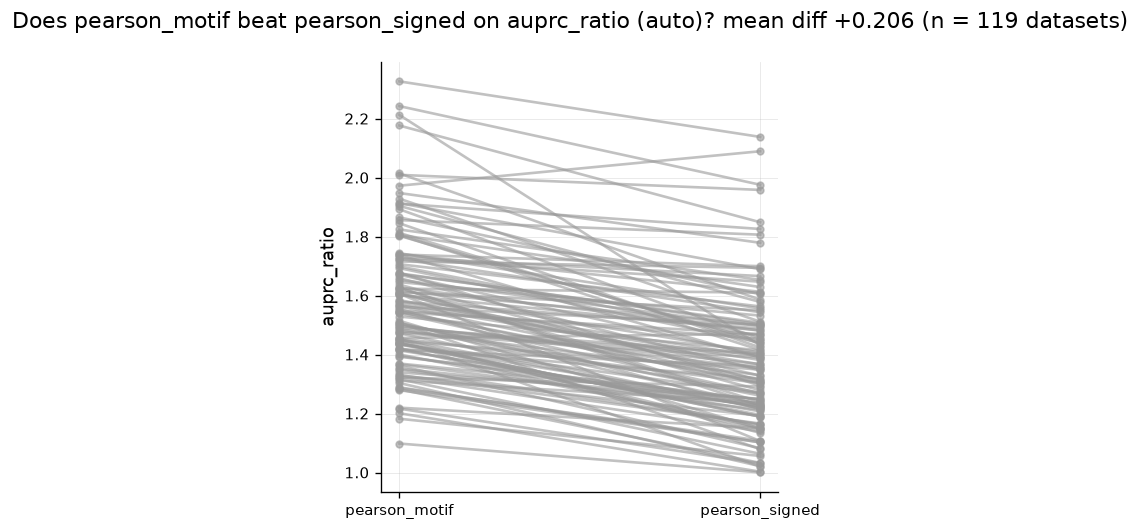
\includegraphics[width=0.85\linewidth]{../viz/lift_pearson_motif_vs_pearson_signed.png}
\caption{-   (n = 119 datasets) - built from  rows/ .json (pearson\_motif vs pearson\_signed)}
\end{figure}
\begin{figure}[H]\centering
\includegraphics[width=0.85\linewidth]{../viz/motif_lift_cxg__10x-3-v2__homo-sapiens__anterior-wall-of-left-ventricl__4ed927e9_pearson_signed.png}
\caption{-   (n = shared TFs) - built from  pearson\_signed.tsv.gz vs pearson\_motif.tsv.gz}
\end{figure}
\begin{figure}[H]\centering
\includegraphics[width=0.85\linewidth]{../viz/motif_lift_cxg__10x-3-v2__homo-sapiens__blood__ae5341b8_pearson_signed.png}
\caption{-   (n = shared TFs) - built from  pearson\_signed.tsv.gz vs pearson\_motif.tsv.gz}
\end{figure}
\begin{figure}[H]\centering
\includegraphics[width=0.85\linewidth]{../viz/motif_lift_cxg__10x-3-v2__homo-sapiens__brain__dc30c3ec_pearson_signed.png}
\caption{-   (n = shared TFs) - built from  pearson\_signed.tsv.gz vs pearson\_motif.tsv.gz}
\end{figure}
\begin{figure}[H]\centering
\includegraphics[width=0.85\linewidth]{../viz/motif_lift_cxg__10x-3-v2__homo-sapiens__breast__9a64bf99_pearson_signed.png}
\caption{-   (n = shared TFs) - built from  pearson\_signed.tsv.gz vs pearson\_motif.tsv.gz}
\end{figure}
\begin{figure}[H]\centering
\includegraphics[width=0.85\linewidth]{../viz/motif_lift_cxg__10x-3-v2__homo-sapiens__caudate-lobe-of-liver__a43aa46b_pearson_signed.png}
\caption{-   (n = shared TFs) - built from  pearson\_signed.tsv.gz vs pearson\_motif.tsv.gz}
\end{figure}
\begin{figure}[H]\centering
\includegraphics[width=0.85\linewidth]{../viz/motif_lift_cxg__10x-3-v2__homo-sapiens__cortex-of-kidney__105c7dad_pearson_signed.png}
\caption{-   (n = shared TFs) - built from  pearson\_signed.tsv.gz vs pearson\_motif.tsv.gz}
\end{figure}
\begin{figure}[H]\centering
\includegraphics[width=0.85\linewidth]{../viz/motif_lift_cxg__10x-3-v2__homo-sapiens__dental-pulp__bdd109f1_pearson_signed.png}
\caption{-   (n = shared TFs) - built from  pearson\_signed.tsv.gz vs pearson\_motif.tsv.gz}
\end{figure}
\begin{figure}[H]\centering
\includegraphics[width=0.85\linewidth]{../viz/motif_lift_cxg__10x-3-v2__homo-sapiens__epithelium-of-rectum__80d7111d_pearson_signed.png}
\caption{-   (n = shared TFs) - built from  pearson\_signed.tsv.gz vs pearson\_motif.tsv.gz}
\end{figure}
\begin{figure}[H]\centering
\includegraphics[width=0.85\linewidth]{../viz/motif_lift_cxg__10x-3-v2__homo-sapiens__fovea-centralis__babbf9f3_pearson_signed.png}
\caption{-   (n = shared TFs) - built from  pearson\_signed.tsv.gz vs pearson\_motif.tsv.gz}
\end{figure}
\begin{figure}[H]\centering
\includegraphics[width=0.85\linewidth]{../viz/motif_lift_cxg__10x-3-v2__homo-sapiens__kidney__8dc29642_pearson_signed.png}
\caption{-   (n = shared TFs) - built from  pearson\_signed.tsv.gz vs pearson\_motif.tsv.gz}
\end{figure}
\begin{figure}[H]\centering
\includegraphics[width=0.85\linewidth]{../viz/motif_lift_cxg__10x-3-v2__homo-sapiens__lung__6e00ccf7_pearson_signed.png}
\caption{-   (n = shared TFs) - built from  pearson\_signed.tsv.gz vs pearson\_motif.tsv.gz}
\end{figure}
\begin{figure}[H]\centering
\includegraphics[width=0.85\linewidth]{../viz/motif_lift_cxg__10x-3-v2__homo-sapiens__mammary-gland-connective-tissu__68b6114f_pearson_signed.png}
\caption{-   (n = shared TFs) - built from  pearson\_signed.tsv.gz vs pearson\_motif.tsv.gz}
\end{figure}
\begin{figure}[H]\centering
\includegraphics[width=0.85\linewidth]{../viz/motif_lift_cxg__10x-3-v2__homo-sapiens__ovary__1f1c5c14_pearson_signed.png}
\caption{-   (n = shared TFs) - built from  pearson\_signed.tsv.gz vs pearson\_motif.tsv.gz}
\end{figure}
\begin{figure}[H]\centering
\includegraphics[width=0.85\linewidth]{../viz/motif_lift_cxg__10x-3-v2__homo-sapiens__respiratory-airway__8fcf0ccc_pearson_signed.png}
\caption{-   (n = shared TFs) - built from  pearson\_signed.tsv.gz vs pearson\_motif.tsv.gz}
\end{figure}
\begin{figure}[H]\centering
\includegraphics[width=0.85\linewidth]{../viz/motif_lift_cxg__10x-3-v2__homo-sapiens__skin-of-prepuce-of-penis__f512b8b6_pearson_signed.png}
\caption{-   (n = shared TFs) - built from  pearson\_signed.tsv.gz vs pearson\_motif.tsv.gz}
\end{figure}
\begin{figure}[H]\centering
\includegraphics[width=0.85\linewidth]{../viz/motif_lift_cxg__10x-3-v2__homo-sapiens__thymus__11ff73e8_pearson_signed.png}
\caption{-   (n = shared TFs) - built from  pearson\_signed.tsv.gz vs pearson\_motif.tsv.gz}
\end{figure}
\begin{figure}[H]\centering
\includegraphics[width=0.85\linewidth]{../viz/motif_lift_cxg__10x-3-v2__homo-sapiens__zone-of-skin__124744b8_pearson_signed.png}
\caption{-   (n = shared TFs) - built from  pearson\_signed.tsv.gz vs pearson\_motif.tsv.gz}
\end{figure}
\begin{figure}[H]\centering
\includegraphics[width=0.85\linewidth]{../viz/motif_lift_cxg__10x-3-v2__mus-musculus__hindlimb-muscle__bedee313_pearson_signed.png}
\caption{-   (n = shared TFs) - built from  pearson\_signed.tsv.gz vs pearson\_motif.tsv.gz}
\end{figure}
\begin{figure}[H]\centering
\includegraphics[width=0.85\linewidth]{../viz/motif_lift_cxg__10x-3-v3__homo-sapiens__abdomen__7b95971d_pearson_signed.png}
\caption{-   (n = shared TFs) - built from  pearson\_signed.tsv.gz vs pearson\_motif.tsv.gz}
\end{figure}
\begin{figure}[H]\centering
\includegraphics[width=0.85\linewidth]{../viz/motif_lift_cxg__10x-3-v3__homo-sapiens__abdomen__97d9238c_pearson_signed.png}
\caption{-   (n = shared TFs) - built from  pearson\_signed.tsv.gz vs pearson\_motif.tsv.gz}
\end{figure}
\begin{figure}[H]\centering
\includegraphics[width=0.85\linewidth]{../viz/motif_lift_cxg__10x-3-v3__homo-sapiens__apex-of-heart__2e9d2f32_pearson_signed.png}
\caption{-   (n = shared TFs) - built from  pearson\_signed.tsv.gz vs pearson\_motif.tsv.gz}
\end{figure}
\begin{figure}[H]\centering
\includegraphics[width=0.85\linewidth]{../viz/motif_lift_cxg__10x-3-v3__homo-sapiens__blood__19e46756_pearson_signed.png}
\caption{-   (n = shared TFs) - built from  pearson\_signed.tsv.gz vs pearson\_motif.tsv.gz}
\end{figure}
\begin{figure}[H]\centering
\includegraphics[width=0.85\linewidth]{../viz/motif_lift_cxg__10x-3-v3__homo-sapiens__blood__20fae564_pearson_signed.png}
\caption{-   (n = shared TFs) - built from  pearson\_signed.tsv.gz vs pearson\_motif.tsv.gz}
\end{figure}
\begin{figure}[H]\centering
\includegraphics[width=0.85\linewidth]{../viz/motif_lift_cxg__10x-3-v3__homo-sapiens__blood__738942eb_pearson_signed.png}
\caption{-   (n = shared TFs) - built from  pearson\_signed.tsv.gz vs pearson\_motif.tsv.gz}
\end{figure}
\begin{figure}[H]\centering
\includegraphics[width=0.85\linewidth]{../viz/motif_lift_cxg__10x-3-v3__homo-sapiens__blood__a199ca73_pearson_signed.png}
\caption{-   (n = shared TFs) - built from  pearson\_signed.tsv.gz vs pearson\_motif.tsv.gz}
\end{figure}
\begin{figure}[H]\centering
\includegraphics[width=0.85\linewidth]{../viz/motif_lift_cxg__10x-3-v3__homo-sapiens__blood__d9f3a82c_pearson_signed.png}
\caption{-   (n = shared TFs) - built from  pearson\_signed.tsv.gz vs pearson\_motif.tsv.gz}
\end{figure}
\begin{figure}[H]\centering
\includegraphics[width=0.85\linewidth]{../viz/motif_lift_cxg__10x-3-v3__homo-sapiens__blood__de2c780c_pearson_signed.png}
\caption{-   (n = shared TFs) - built from  pearson\_signed.tsv.gz vs pearson\_motif.tsv.gz}
\end{figure}
\begin{figure}[H]\centering
\includegraphics[width=0.85\linewidth]{../viz/motif_lift_cxg__10x-3-v3__homo-sapiens__bone-marrow__343ff97c_pearson_signed.png}
\caption{-   (n = shared TFs) - built from  pearson\_signed.tsv.gz vs pearson\_motif.tsv.gz}
\end{figure}
\begin{figure}[H]\centering
\includegraphics[width=0.85\linewidth]{../viz/motif_lift_cxg__10x-3-v3__homo-sapiens__breast__24ec2dc5_pearson_signed.png}
\caption{-   (n = shared TFs) - built from  pearson\_signed.tsv.gz vs pearson\_motif.tsv.gz}
\end{figure}
\begin{figure}[H]\centering
\includegraphics[width=0.85\linewidth]{../viz/motif_lift_cxg__10x-3-v3__homo-sapiens__brodmann-1909-area-13__f16f4108_pearson_signed.png}
\caption{-   (n = shared TFs) - built from  pearson\_signed.tsv.gz vs pearson\_motif.tsv.gz}
\end{figure}
\begin{figure}[H]\centering
\includegraphics[width=0.85\linewidth]{../viz/motif_lift_cxg__10x-3-v3__homo-sapiens__brodmann-1909-area-4__c8f83821_pearson_signed.png}
\caption{-   (n = shared TFs) - built from  pearson\_signed.tsv.gz vs pearson\_motif.tsv.gz}
\end{figure}
\begin{figure}[H]\centering
\includegraphics[width=0.85\linewidth]{../viz/motif_lift_cxg__10x-3-v3__homo-sapiens__brown-preadipocyte__137ca42b_pearson_signed.png}
\caption{-   (n = shared TFs) - built from  pearson\_signed.tsv.gz vs pearson\_motif.tsv.gz}
\end{figure}
\begin{figure}[H]\centering
\includegraphics[width=0.85\linewidth]{../viz/motif_lift_cxg__10x-3-v3__homo-sapiens__calcaneal-tendon__ef0fc6ac_pearson_signed.png}
\caption{-   (n = shared TFs) - built from  pearson\_signed.tsv.gz vs pearson\_motif.tsv.gz}
\end{figure}
\begin{figure}[H]\centering
\includegraphics[width=0.85\linewidth]{../viz/motif_lift_cxg__10x-3-v3__homo-sapiens__calcaneal-tendon__f641d68a_pearson_signed.png}
\caption{-   (n = shared TFs) - built from  pearson\_signed.tsv.gz vs pearson\_motif.tsv.gz}
\end{figure}
\begin{figure}[H]\centering
\includegraphics[width=0.85\linewidth]{../viz/motif_lift_cxg__10x-3-v3__homo-sapiens__caudate-nucleus__c893ddc3_pearson_signed.png}
\caption{-   (n = shared TFs) - built from  pearson\_signed.tsv.gz vs pearson\_motif.tsv.gz}
\end{figure}
\begin{figure}[H]\centering
\includegraphics[width=0.85\linewidth]{../viz/motif_lift_cxg__10x-3-v3__homo-sapiens__cerebellum__be884a28_pearson_signed.png}
\caption{-   (n = shared TFs) - built from  pearson\_signed.tsv.gz vs pearson\_motif.tsv.gz}
\end{figure}
\begin{figure}[H]\centering
\includegraphics[width=0.85\linewidth]{../viz/motif_lift_cxg__10x-3-v3__homo-sapiens__cornea__8058d760_pearson_signed.png}
\caption{-   (n = shared TFs) - built from  pearson\_signed.tsv.gz vs pearson\_motif.tsv.gz}
\end{figure}
\begin{figure}[H]\centering
\includegraphics[width=0.85\linewidth]{../viz/motif_lift_cxg__10x-3-v3__homo-sapiens__cortex-of-kidney__07854d9c_pearson_signed.png}
\caption{-   (n = shared TFs) - built from  pearson\_signed.tsv.gz vs pearson\_motif.tsv.gz}
\end{figure}
\begin{figure}[H]\centering
\includegraphics[width=0.85\linewidth]{../viz/motif_lift_cxg__10x-3-v3__homo-sapiens__cortex-of-kidney__0bae7ebf_pearson_signed.png}
\caption{-   (n = shared TFs) - built from  pearson\_signed.tsv.gz vs pearson\_motif.tsv.gz}
\end{figure}
\begin{figure}[H]\centering
\includegraphics[width=0.85\linewidth]{../viz/motif_lift_cxg__10x-3-v3__homo-sapiens__cranial-nerve-ii__374edd6c_pearson_signed.png}
\caption{-   (n = shared TFs) - built from  pearson\_signed.tsv.gz vs pearson\_motif.tsv.gz}
\end{figure}
\begin{figure}[H]\centering
\includegraphics[width=0.85\linewidth]{../viz/motif_lift_cxg__10x-3-v3__homo-sapiens__cranial-nerve-ii__9f1a899f_pearson_signed.png}
\caption{-   (n = shared TFs) - built from  pearson\_signed.tsv.gz vs pearson\_motif.tsv.gz}
\end{figure}
\begin{figure}[H]\centering
\includegraphics[width=0.85\linewidth]{../viz/motif_lift_cxg__10x-3-v3__homo-sapiens__dome-of-urinary-bladder__601c7454_pearson_signed.png}
\caption{-   (n = shared TFs) - built from  pearson\_signed.tsv.gz vs pearson\_motif.tsv.gz}
\end{figure}
\begin{figure}[H]\centering
\includegraphics[width=0.85\linewidth]{../viz/motif_lift_cxg__10x-3-v3__homo-sapiens__endometrium__76150f40_pearson_signed.png}
\caption{-   (n = shared TFs) - built from  pearson\_signed.tsv.gz vs pearson\_motif.tsv.gz}
\end{figure}
\begin{figure}[H]\centering
\includegraphics[width=0.85\linewidth]{../viz/motif_lift_cxg__10x-3-v3__homo-sapiens__endometrium__7a419302_pearson_signed.png}
\caption{-   (n = shared TFs) - built from  pearson\_signed.tsv.gz vs pearson\_motif.tsv.gz}
\end{figure}
\begin{figure}[H]\centering
\includegraphics[width=0.85\linewidth]{../viz/motif_lift_cxg__10x-3-v3__homo-sapiens__entorhinal-cortex__24584be9_pearson_signed.png}
\caption{-   (n = shared TFs) - built from  pearson\_signed.tsv.gz vs pearson\_motif.tsv.gz}
\end{figure}
\begin{figure}[H]\centering
\includegraphics[width=0.85\linewidth]{../viz/motif_lift_cxg__10x-3-v3__homo-sapiens__fallopian-tube__30f5e171_pearson_signed.png}
\caption{-   (n = shared TFs) - built from  pearson\_signed.tsv.gz vs pearson\_motif.tsv.gz}
\end{figure}
\begin{figure}[H]\centering
\includegraphics[width=0.85\linewidth]{../viz/motif_lift_cxg__10x-3-v3__homo-sapiens__fovea-centralis__11ef37ee_pearson_signed.png}
\caption{-   (n = shared TFs) - built from  pearson\_signed.tsv.gz vs pearson\_motif.tsv.gz}
\end{figure}
\begin{figure}[H]\centering
\includegraphics[width=0.85\linewidth]{../viz/motif_lift_cxg__10x-3-v3__homo-sapiens__fovea-centralis__af8b241a_pearson_signed.png}
\caption{-   (n = shared TFs) - built from  pearson\_signed.tsv.gz vs pearson\_motif.tsv.gz}
\end{figure}
\begin{figure}[H]\centering
\includegraphics[width=0.85\linewidth]{../viz/motif_lift_cxg__10x-3-v3__homo-sapiens__fovea-centralis__e404d417_pearson_signed.png}
\caption{-   (n = shared TFs) - built from  pearson\_signed.tsv.gz vs pearson\_motif.tsv.gz}
\end{figure}
\begin{figure}[H]\centering
\includegraphics[width=0.85\linewidth]{../viz/motif_lift_cxg__10x-3-v3__homo-sapiens__fovea-centralis__f5be9ed2_pearson_signed.png}
\caption{-   (n = shared TFs) - built from  pearson\_signed.tsv.gz vs pearson\_motif.tsv.gz}
\end{figure}
\begin{figure}[H]\centering
\includegraphics[width=0.85\linewidth]{../viz/motif_lift_cxg__10x-3-v3__homo-sapiens__heart-left-ventricle__f15e263b_pearson_signed.png}
\caption{-   (n = shared TFs) - built from  pearson\_signed.tsv.gz vs pearson\_motif.tsv.gz}
\end{figure}
\begin{figure}[H]\centering
\includegraphics[width=0.85\linewidth]{../viz/motif_lift_cxg__10x-3-v3__homo-sapiens__kidney__ea01c125_pearson_signed.png}
\caption{-   (n = shared TFs) - built from  pearson\_signed.tsv.gz vs pearson\_motif.tsv.gz}
\end{figure}
\begin{figure}[H]\centering
\includegraphics[width=0.85\linewidth]{../viz/motif_lift_cxg__10x-3-v3__homo-sapiens__left-atrium-auricular-region__87a06a2a_pearson_signed.png}
\caption{-   (n = shared TFs) - built from  pearson\_signed.tsv.gz vs pearson\_motif.tsv.gz}
\end{figure}
\begin{figure}[H]\centering
\includegraphics[width=0.85\linewidth]{../viz/motif_lift_cxg__10x-3-v3__homo-sapiens__lens-of-camera-type-eye__489318a0_pearson_signed.png}
\caption{-   (n = shared TFs) - built from  pearson\_signed.tsv.gz vs pearson\_motif.tsv.gz}
\end{figure}
\begin{figure}[H]\centering
\includegraphics[width=0.85\linewidth]{../viz/motif_lift_cxg__10x-3-v3__homo-sapiens__liver__0bbf93aa_pearson_signed.png}
\caption{-   (n = shared TFs) - built from  pearson\_signed.tsv.gz vs pearson\_motif.tsv.gz}
\end{figure}
\begin{figure}[H]\centering
\includegraphics[width=0.85\linewidth]{../viz/motif_lift_cxg__10x-3-v3__homo-sapiens__liver__ec6ceff8_pearson_signed.png}
\caption{-   (n = shared TFs) - built from  pearson\_signed.tsv.gz vs pearson\_motif.tsv.gz}
\end{figure}
\begin{figure}[H]\centering
\includegraphics[width=0.85\linewidth]{../viz/motif_lift_cxg__10x-3-v3__homo-sapiens__lung-parenchyma__01ff5cf0_pearson_signed.png}
\caption{-   (n = shared TFs) - built from  pearson\_signed.tsv.gz vs pearson\_motif.tsv.gz}
\end{figure}
\begin{figure}[H]\centering
\includegraphics[width=0.85\linewidth]{../viz/motif_lift_cxg__10x-3-v3__homo-sapiens__lung-parenchyma__8fbed309_pearson_signed.png}
\caption{-   (n = shared TFs) - built from  pearson\_signed.tsv.gz vs pearson\_motif.tsv.gz}
\end{figure}
\begin{figure}[H]\centering
\includegraphics[width=0.85\linewidth]{../viz/motif_lift_cxg__10x-3-v3__homo-sapiens__lung__6ba45a2b_pearson_signed.png}
\caption{-   (n = shared TFs) - built from  pearson\_signed.tsv.gz vs pearson\_motif.tsv.gz}
\end{figure}
\begin{figure}[H]\centering
\includegraphics[width=0.85\linewidth]{../viz/motif_lift_cxg__10x-3-v3__homo-sapiens__lung__d8da613f_pearson_signed.png}
\caption{-   (n = shared TFs) - built from  pearson\_signed.tsv.gz vs pearson\_motif.tsv.gz}
\end{figure}
\begin{figure}[H]\centering
\includegraphics[width=0.85\linewidth]{../viz/motif_lift_cxg__10x-3-v3__homo-sapiens__mesenteric-artery__42b6a476_pearson_signed.png}
\caption{-   (n = shared TFs) - built from  pearson\_signed.tsv.gz vs pearson\_motif.tsv.gz}
\end{figure}
\begin{figure}[H]\centering
\includegraphics[width=0.85\linewidth]{../viz/motif_lift_cxg__10x-3-v3__homo-sapiens__minor-salivary-gland__9aef5aa0_pearson_signed.png}
\caption{-   (n = shared TFs) - built from  pearson\_signed.tsv.gz vs pearson\_motif.tsv.gz}
\end{figure}
\begin{figure}[H]\centering
\includegraphics[width=0.85\linewidth]{../viz/motif_lift_cxg__10x-3-v3__homo-sapiens__neocortex__3a8aec06_pearson_signed.png}
\caption{-   (n = shared TFs) - built from  pearson\_signed.tsv.gz vs pearson\_motif.tsv.gz}
\end{figure}
\begin{figure}[H]\centering
\includegraphics[width=0.85\linewidth]{../viz/motif_lift_cxg__10x-3-v3__homo-sapiens__neocortex__4859642c_pearson_signed.png}
\caption{-   (n = shared TFs) - built from  pearson\_signed.tsv.gz vs pearson\_motif.tsv.gz}
\end{figure}
\begin{figure}[H]\centering
\includegraphics[width=0.85\linewidth]{../viz/motif_lift_cxg__10x-3-v3__homo-sapiens__occipital-cortex__e6361237_pearson_signed.png}
\caption{-   (n = shared TFs) - built from  pearson\_signed.tsv.gz vs pearson\_motif.tsv.gz}
\end{figure}
\begin{figure}[H]\centering
\includegraphics[width=0.85\linewidth]{../viz/motif_lift_cxg__10x-3-v3__homo-sapiens__oropharynx__b6b5ea88_pearson_signed.png}
\caption{-   (n = shared TFs) - built from  pearson\_signed.tsv.gz vs pearson\_motif.tsv.gz}
\end{figure}
\begin{figure}[H]\centering
\includegraphics[width=0.85\linewidth]{../viz/motif_lift_cxg__10x-3-v3__homo-sapiens__ovary__3a702020_pearson_signed.png}
\caption{-   (n = shared TFs) - built from  pearson\_signed.tsv.gz vs pearson\_motif.tsv.gz}
\end{figure}
\begin{figure}[H]\centering
\includegraphics[width=0.85\linewidth]{../viz/motif_lift_cxg__10x-3-v3__homo-sapiens__ovary__a9bedd04_pearson_signed.png}
\caption{-   (n = shared TFs) - built from  pearson\_signed.tsv.gz vs pearson\_motif.tsv.gz}
\end{figure}
\begin{figure}[H]\centering
\includegraphics[width=0.85\linewidth]{../viz/motif_lift_cxg__10x-3-v3__homo-sapiens__placenta__b7efc0ba_pearson_signed.png}
\caption{-   (n = shared TFs) - built from  pearson\_signed.tsv.gz vs pearson\_motif.tsv.gz}
\end{figure}
\begin{figure}[H]\centering
\includegraphics[width=0.85\linewidth]{../viz/motif_lift_cxg__10x-3-v3__homo-sapiens__prefrontal-cortex__fe2eecbc_pearson_signed.png}
\caption{-   (n = shared TFs) - built from  pearson\_signed.tsv.gz vs pearson\_motif.tsv.gz}
\end{figure}
\begin{figure}[H]\centering
\includegraphics[width=0.85\linewidth]{../viz/motif_lift_cxg__10x-3-v3__homo-sapiens__right-atrium-auricular-region__8f4f8502_pearson_signed.png}
\caption{-   (n = shared TFs) - built from  pearson\_signed.tsv.gz vs pearson\_motif.tsv.gz}
\end{figure}
\begin{figure}[H]\centering
\includegraphics[width=0.85\linewidth]{../viz/motif_lift_cxg__10x-3-v3__homo-sapiens__right-temporal-lobe__145dcf6a_pearson_signed.png}
\caption{-   (n = shared TFs) - built from  pearson\_signed.tsv.gz vs pearson\_motif.tsv.gz}
\end{figure}
\begin{figure}[H]\centering
\includegraphics[width=0.85\linewidth]{../viz/motif_lift_cxg__10x-3-v3__homo-sapiens__skin-of-body__b796f27e_pearson_signed.png}
\caption{-   (n = shared TFs) - built from  pearson\_signed.tsv.gz vs pearson\_motif.tsv.gz}
\end{figure}
\begin{figure}[H]\centering
\includegraphics[width=0.85\linewidth]{../viz/motif_lift_cxg__10x-3-v3__homo-sapiens__tendon-of-semitendinosus__06ef6b36_pearson_signed.png}
\caption{-   (n = shared TFs) - built from  pearson\_signed.tsv.gz vs pearson\_motif.tsv.gz}
\end{figure}
\begin{figure}[H]\centering
\includegraphics[width=0.85\linewidth]{../viz/motif_lift_cxg__10x-3-v3__homo-sapiens__upper-lobe-of-left-lung__2ac76f1b_pearson_signed.png}
\caption{-   (n = shared TFs) - built from  pearson\_signed.tsv.gz vs pearson\_motif.tsv.gz}
\end{figure}
\begin{figure}[H]\centering
\includegraphics[width=0.85\linewidth]{../viz/motif_lift_cxg__10x-3-v3__homo-sapiens__visceral-fat__1405dd3e_pearson_signed.png}
\caption{-   (n = shared TFs) - built from  pearson\_signed.tsv.gz vs pearson\_motif.tsv.gz}
\end{figure}
\begin{figure}[H]\centering
\includegraphics[width=0.85\linewidth]{../viz/motif_lift_cxg__10x-3-v3__mus-musculus__aorta__f7417545_pearson_signed.png}
\caption{-   (n = shared TFs) - built from  pearson\_signed.tsv.gz vs pearson\_motif.tsv.gz}
\end{figure}
\begin{figure}[H]\centering
\includegraphics[width=0.85\linewidth]{../viz/motif_lift_cxg__10x-3-v3__mus-musculus__brain-gray-matter__6347cc90_pearson_signed.png}
\caption{-   (n = shared TFs) - built from  pearson\_signed.tsv.gz vs pearson\_motif.tsv.gz}
\end{figure}
\begin{figure}[H]\centering
\includegraphics[width=0.85\linewidth]{../viz/motif_lift_cxg__10x-3-v3__mus-musculus__brain__e056b20b_pearson_signed.png}
\caption{-   (n = shared TFs) - built from  pearson\_signed.tsv.gz vs pearson\_motif.tsv.gz}
\end{figure}
\begin{figure}[H]\centering
\includegraphics[width=0.85\linewidth]{../viz/motif_lift_cxg__10x-3-v3__mus-musculus__cerebral-cortex__0e1c7067_pearson_signed.png}
\caption{-   (n = shared TFs) - built from  pearson\_signed.tsv.gz vs pearson\_motif.tsv.gz}
\end{figure}
\begin{figure}[H]\centering
\includegraphics[width=0.85\linewidth]{../viz/motif_lift_cxg__10x-3-v3__mus-musculus__cerebral-cortex__12990215_pearson_signed.png}
\caption{-   (n = shared TFs) - built from  pearson\_signed.tsv.gz vs pearson\_motif.tsv.gz}
\end{figure}
\begin{figure}[H]\centering
\includegraphics[width=0.85\linewidth]{../viz/motif_lift_cxg__10x-3-v3__mus-musculus__gastrocnemius__2ab892f9_pearson_signed.png}
\caption{-   (n = shared TFs) - built from  pearson\_signed.tsv.gz vs pearson\_motif.tsv.gz}
\end{figure}
\begin{figure}[H]\centering
\includegraphics[width=0.85\linewidth]{../viz/motif_lift_cxg__10x-3-v3__mus-musculus__gingiva__e04cb7d9_pearson_signed.png}
\caption{-   (n = shared TFs) - built from  pearson\_signed.tsv.gz vs pearson\_motif.tsv.gz}
\end{figure}
\begin{figure}[H]\centering
\includegraphics[width=0.85\linewidth]{../viz/motif_lift_cxg__10x-3-v3__mus-musculus__liver__e9de826e_pearson_signed.png}
\caption{-   (n = shared TFs) - built from  pearson\_signed.tsv.gz vs pearson\_motif.tsv.gz}
\end{figure}
\begin{figure}[H]\centering
\includegraphics[width=0.85\linewidth]{../viz/motif_lift_cxg__10x-3-v3__mus-musculus__middle-lobe-of-right-lung__89840cec_pearson_signed.png}
\caption{-   (n = shared TFs) - built from  pearson\_signed.tsv.gz vs pearson\_motif.tsv.gz}
\end{figure}
\begin{figure}[H]\centering
\includegraphics[width=0.85\linewidth]{../viz/motif_lift_cxg__10x-3-v3__mus-musculus__ovary__55d66f2a_pearson_signed.png}
\caption{-   (n = shared TFs) - built from  pearson\_signed.tsv.gz vs pearson\_motif.tsv.gz}
\end{figure}
\begin{figure}[H]\centering
\includegraphics[width=0.85\linewidth]{../viz/motif_lift_cxg__10x-3-v3__mus-musculus__tracheal-epithelial-cell__732a691e_pearson_signed.png}
\caption{-   (n = shared TFs) - built from  pearson\_signed.tsv.gz vs pearson\_motif.tsv.gz}
\end{figure}
\begin{figure}[H]\centering
\includegraphics[width=0.85\linewidth]{../viz/motif_lift_cxg__10x-5-transcription-profiling__homo-sapiens__adrenal-tissue__5af90777_pearson_signed.png}
\caption{-   (n = shared TFs) - built from  pearson\_signed.tsv.gz vs pearson\_motif.tsv.gz}
\end{figure}
\begin{figure}[H]\centering
\includegraphics[width=0.85\linewidth]{../viz/motif_lift_cxg__10x-5-transcription-profiling__homo-sapiens__lung__8dc858b0_pearson_signed.png}
\caption{-   (n = shared TFs) - built from  pearson\_signed.tsv.gz vs pearson\_motif.tsv.gz}
\end{figure}
\begin{figure}[H]\centering
\includegraphics[width=0.85\linewidth]{../viz/motif_lift_cxg__10x-5-v1__homo-sapiens__blood__5b25a46f_pearson_signed.png}
\caption{-   (n = shared TFs) - built from  pearson\_signed.tsv.gz vs pearson\_motif.tsv.gz}
\end{figure}
\begin{figure}[H]\centering
\includegraphics[width=0.85\linewidth]{../viz/motif_lift_cxg__10x-5-v1__homo-sapiens__blood__c2a461b1_pearson_signed.png}
\caption{-   (n = shared TFs) - built from  pearson\_signed.tsv.gz vs pearson\_motif.tsv.gz}
\end{figure}
\begin{figure}[H]\centering
\includegraphics[width=0.85\linewidth]{../viz/motif_lift_cxg__10x-5-v1__homo-sapiens__blood__fa8605cf_pearson_signed.png}
\caption{-   (n = shared TFs) - built from  pearson\_signed.tsv.gz vs pearson\_motif.tsv.gz}
\end{figure}
\begin{figure}[H]\centering
\includegraphics[width=0.85\linewidth]{../viz/motif_lift_cxg__10x-5-v1__homo-sapiens__lymph-node__99950e99_pearson_signed.png}
\caption{-   (n = shared TFs) - built from  pearson\_signed.tsv.gz vs pearson\_motif.tsv.gz}
\end{figure}
\begin{figure}[H]\centering
\includegraphics[width=0.85\linewidth]{../viz/motif_lift_cxg__10x-5-v1__homo-sapiens__t-cell__0c774045_pearson_signed.png}
\caption{-   (n = shared TFs) - built from  pearson\_signed.tsv.gz vs pearson\_motif.tsv.gz}
\end{figure}
\begin{figure}[H]\centering
\includegraphics[width=0.85\linewidth]{../viz/motif_lift_cxg__10x-5-v1__homo-sapiens__t-cell__460dfe21_pearson_signed.png}
\caption{-   (n = shared TFs) - built from  pearson\_signed.tsv.gz vs pearson\_motif.tsv.gz}
\end{figure}
\begin{figure}[H]\centering
\includegraphics[width=0.85\linewidth]{../viz/motif_lift_cxg__10x-5-v1__homo-sapiens__thymus__8d73847b_pearson_signed.png}
\caption{-   (n = shared TFs) - built from  pearson\_signed.tsv.gz vs pearson\_motif.tsv.gz}
\end{figure}
\begin{figure}[H]\centering
\includegraphics[width=0.85\linewidth]{../viz/motif_lift_cxg__10x-5-v1__mus-musculus__gonad__a13bda79_pearson_signed.png}
\caption{-   (n = shared TFs) - built from  pearson\_signed.tsv.gz vs pearson\_motif.tsv.gz}
\end{figure}
\begin{figure}[H]\centering
\includegraphics[width=0.85\linewidth]{../viz/motif_lift_cxg__10x-5-v2__homo-sapiens__blood__30c2a6fd_pearson_signed.png}
\caption{-   (n = shared TFs) - built from  pearson\_signed.tsv.gz vs pearson\_motif.tsv.gz}
\end{figure}
\begin{figure}[H]\centering
\includegraphics[width=0.85\linewidth]{../viz/motif_lift_cxg__10x-5-v2__homo-sapiens__blood__bd65a70f_pearson_signed.png}
\caption{-   (n = shared TFs) - built from  pearson\_signed.tsv.gz vs pearson\_motif.tsv.gz}
\end{figure}
\begin{figure}[H]\centering
\includegraphics[width=0.85\linewidth]{../viz/motif_lift_cxg__10x-multiome__homo-sapiens__amygdala__835fa5c4_pearson_signed.png}
\caption{-   (n = shared TFs) - built from  pearson\_signed.tsv.gz vs pearson\_motif.tsv.gz}
\end{figure}
\begin{figure}[H]\centering
\includegraphics[width=0.85\linewidth]{../viz/motif_lift_cxg__10x-multiome__homo-sapiens__anterior-cingulate-cortex__56a4bc14_pearson_signed.png}
\caption{-   (n = shared TFs) - built from  pearson\_signed.tsv.gz vs pearson\_motif.tsv.gz}
\end{figure}
\begin{figure}[H]\centering
\includegraphics[width=0.85\linewidth]{../viz/motif_lift_cxg__10x-multiome__homo-sapiens__frontal-lobe__01b84709_pearson_signed.png}
\caption{-   (n = shared TFs) - built from  pearson\_signed.tsv.gz vs pearson\_motif.tsv.gz}
\end{figure}
\begin{figure}[H]\centering
\includegraphics[width=0.85\linewidth]{../viz/motif_lift_cxg__10x-multiome__homo-sapiens__kidney__867757c1_pearson_signed.png}
\caption{-   (n = shared TFs) - built from  pearson\_signed.tsv.gz vs pearson\_motif.tsv.gz}
\end{figure}
\begin{figure}[H]\centering
\includegraphics[width=0.85\linewidth]{../viz/motif_lift_cxg__10x-multiome__homo-sapiens__retina__322c816f_pearson_signed.png}
\caption{-   (n = shared TFs) - built from  pearson\_signed.tsv.gz vs pearson\_motif.tsv.gz}
\end{figure}
\begin{figure}[H]\centering
\includegraphics[width=0.85\linewidth]{../viz/motif_lift_cxg__10x-multiome__mus-musculus__kidney__25818bf7_pearson_signed.png}
\caption{-   (n = shared TFs) - built from  pearson\_signed.tsv.gz vs pearson\_motif.tsv.gz}
\end{figure}
\begin{figure}[H]\centering
\includegraphics[width=0.85\linewidth]{../viz/motif_lift_cxg__10x-next-gem-flex-v1__homo-sapiens__endometrium__fb90c70d_pearson_signed.png}
\caption{-   (n = shared TFs) - built from  pearson\_signed.tsv.gz vs pearson\_motif.tsv.gz}
\end{figure}
\begin{figure}[H]\centering
\includegraphics[width=0.85\linewidth]{../viz/motif_lift_cxg__10x-next-gem-flex-v1__homo-sapiens__parenchyma-of-mammary-gland__fbdd8c17_pearson_signed.png}
\caption{-   (n = shared TFs) - built from  pearson\_signed.tsv.gz vs pearson\_motif.tsv.gz}
\end{figure}
\begin{figure}[H]\centering
\includegraphics[width=0.85\linewidth]{../viz/motif_lift_cxg__asteria-scrna-seq-kit__homo-sapiens__blood__27d3952f_pearson_signed.png}
\caption{-   (n = shared TFs) - built from  pearson\_signed.tsv.gz vs pearson\_motif.tsv.gz}
\end{figure}
\begin{figure}[H]\centering
\includegraphics[width=0.85\linewidth]{../viz/motif_lift_cxg__bd-rhapsody-whole-transcriptome-analysis__homo-sapiens__liver__e3ed2ba4_pearson_signed.png}
\caption{-   (n = shared TFs) - built from  pearson\_signed.tsv.gz vs pearson\_motif.tsv.gz}
\end{figure}
\begin{figure}[H]\centering
\includegraphics[width=0.85\linewidth]{../viz/motif_lift_cxg__mars-seq__homo-sapiens__bone-marrow__e22482ee_pearson_signed.png}
\caption{-   (n = shared TFs) - built from  pearson\_signed.tsv.gz vs pearson\_motif.tsv.gz}
\end{figure}
\begin{figure}[H]\centering
\includegraphics[width=0.85\linewidth]{../viz/motif_lift_cxg__mct-seq__homo-sapiens__brodmann-1909-area-46__43aa19d2_pearson_signed.png}
\caption{-   (n = shared TFs) - built from  pearson\_signed.tsv.gz vs pearson\_motif.tsv.gz}
\end{figure}
\begin{figure}[H]\centering
\includegraphics[width=0.85\linewidth]{../viz/motif_lift_cxg__sci-plex__homo-sapiens__k-562__38a78e91_pearson_signed.png}
\caption{-   (n = shared TFs) - built from  pearson\_signed.tsv.gz vs pearson\_motif.tsv.gz}
\end{figure}
\begin{figure}[H]\centering
\includegraphics[width=0.85\linewidth]{../viz/motif_lift_cxg__seq-well-s3__homo-sapiens__nasopharynx__13b61a7d_pearson_signed.png}
\caption{-   (n = shared TFs) - built from  pearson\_signed.tsv.gz vs pearson\_motif.tsv.gz}
\end{figure}
\begin{figure}[H]\centering
\includegraphics[width=0.85\linewidth]{../viz/motif_lift_cxg__seq-well__homo-sapiens__blood__456e8b9b_pearson_signed.png}
\caption{-   (n = shared TFs) - built from  pearson\_signed.tsv.gz vs pearson\_motif.tsv.gz}
\end{figure}
\begin{figure}[H]\centering
\includegraphics[width=0.85\linewidth]{../viz/motif_lift_cxg__smart-seq-v4__mus-musculus__primary-motor-cortex__1304e107_pearson_signed.png}
\caption{-   (n = shared TFs) - built from  pearson\_signed.tsv.gz vs pearson\_motif.tsv.gz}
\end{figure}
\begin{figure}[H]\centering
\includegraphics[width=0.85\linewidth]{../viz/motif_lift_cxg__smart-seq2__homo-sapiens__blood__e04daea4_pearson_signed.png}
\caption{-   (n = shared TFs) - built from  pearson\_signed.tsv.gz vs pearson\_motif.tsv.gz}
\end{figure}
\begin{figure}[H]\centering
\includegraphics[width=0.85\linewidth]{../viz/motif_lift_cxg__smart-seq2__homo-sapiens__heart-left-ventricle__07e6773a_pearson_signed.png}
\caption{-   (n = shared TFs) - built from  pearson\_signed.tsv.gz vs pearson\_motif.tsv.gz}
\end{figure}
\begin{figure}[H]\centering
\includegraphics[width=0.85\linewidth]{../viz/motif_lift_cxg__smart-seq__mus-musculus__primary-visual-cortex__3a15ab1c_pearson_signed.png}
\caption{-   (n = shared TFs) - built from  pearson\_signed.tsv.gz vs pearson\_motif.tsv.gz}
\end{figure}
\begin{figure}[H]\centering
\includegraphics[width=0.85\linewidth]{../viz/motif_lift_cxg__split-seq__homo-sapiens__cerebellum__b2dda353_pearson_signed.png}
\caption{-   (n = shared TFs) - built from  pearson\_signed.tsv.gz vs pearson\_motif.tsv.gz}
\end{figure}
\begin{figure}[H]\centering
\includegraphics[width=0.85\linewidth]{../viz/network_cxg__10x-3-v2__homo-sapiens__anterior-wall-of-left-ventricl__4ed927e9.png}
\caption{-   (n = 60 edges) - built from  pearson\_motif.tsv.gz}
\end{figure}
\begin{figure}[H]\centering
\includegraphics[width=0.85\linewidth]{../viz/network_cxg__10x-3-v2__homo-sapiens__blood__ae5341b8.png}
\caption{-   (n = 60 edges) - built from  pearson\_motif.tsv.gz}
\end{figure}
\begin{figure}[H]\centering
\includegraphics[width=0.85\linewidth]{../viz/network_cxg__10x-3-v2__homo-sapiens__brain__dc30c3ec.png}
\caption{-   (n = 60 edges) - built from  pearson\_motif.tsv.gz}
\end{figure}
\begin{figure}[H]\centering
\includegraphics[width=0.85\linewidth]{../viz/network_cxg__10x-3-v2__homo-sapiens__breast__9a64bf99.png}
\caption{-   (n = 60 edges) - built from  pearson\_motif.tsv.gz}
\end{figure}
\begin{figure}[H]\centering
\includegraphics[width=0.85\linewidth]{../viz/network_cxg__10x-3-v2__homo-sapiens__caudate-lobe-of-liver__a43aa46b.png}
\caption{-   (n = 60 edges) - built from  pearson\_motif.tsv.gz}
\end{figure}
\begin{figure}[H]\centering
\includegraphics[width=0.85\linewidth]{../viz/network_cxg__10x-3-v2__homo-sapiens__cortex-of-kidney__105c7dad.png}
\caption{-   (n = 60 edges) - built from  pearson\_motif.tsv.gz}
\end{figure}
\begin{figure}[H]\centering
\includegraphics[width=0.85\linewidth]{../viz/network_cxg__10x-3-v2__homo-sapiens__dental-pulp__bdd109f1.png}
\caption{-   (n = 60 edges) - built from  pearson\_motif.tsv.gz}
\end{figure}
\begin{figure}[H]\centering
\includegraphics[width=0.85\linewidth]{../viz/network_cxg__10x-3-v2__homo-sapiens__epithelium-of-rectum__80d7111d.png}
\caption{-   (n = 60 edges) - built from  pearson\_motif.tsv.gz}
\end{figure}
\begin{figure}[H]\centering
\includegraphics[width=0.85\linewidth]{../viz/network_cxg__10x-3-v2__homo-sapiens__fovea-centralis__babbf9f3.png}
\caption{-   (n = 60 edges) - built from  pearson\_motif.tsv.gz}
\end{figure}
\begin{figure}[H]\centering
\includegraphics[width=0.85\linewidth]{../viz/network_cxg__10x-3-v2__homo-sapiens__kidney__8dc29642.png}
\caption{-   (n = 60 edges) - built from  pearson\_motif.tsv.gz}
\end{figure}
\begin{figure}[H]\centering
\includegraphics[width=0.85\linewidth]{../viz/network_cxg__10x-3-v2__homo-sapiens__lung__6e00ccf7.png}
\caption{-   (n = 60 edges) - built from  pearson\_motif.tsv.gz}
\end{figure}
\begin{figure}[H]\centering
\includegraphics[width=0.85\linewidth]{../viz/network_cxg__10x-3-v2__homo-sapiens__mammary-gland-connective-tissu__68b6114f.png}
\caption{-   (n = 60 edges) - built from  pearson\_motif.tsv.gz}
\end{figure}
\begin{figure}[H]\centering
\includegraphics[width=0.85\linewidth]{../viz/network_cxg__10x-3-v2__homo-sapiens__ovary__1f1c5c14.png}
\caption{-   (n = 60 edges) - built from  pearson\_motif.tsv.gz}
\end{figure}
\begin{figure}[H]\centering
\includegraphics[width=0.85\linewidth]{../viz/network_cxg__10x-3-v2__homo-sapiens__respiratory-airway__8fcf0ccc.png}
\caption{-   (n = 60 edges) - built from  pearson\_motif.tsv.gz}
\end{figure}
\begin{figure}[H]\centering
\includegraphics[width=0.85\linewidth]{../viz/network_cxg__10x-3-v2__homo-sapiens__skin-of-prepuce-of-penis__f512b8b6.png}
\caption{-   (n = 60 edges) - built from  pearson\_motif.tsv.gz}
\end{figure}
\begin{figure}[H]\centering
\includegraphics[width=0.85\linewidth]{../viz/network_cxg__10x-3-v2__homo-sapiens__thymus__11ff73e8.png}
\caption{-   (n = 60 edges) - built from  pearson\_motif.tsv.gz}
\end{figure}
\begin{figure}[H]\centering
\includegraphics[width=0.85\linewidth]{../viz/network_cxg__10x-3-v2__homo-sapiens__zone-of-skin__124744b8.png}
\caption{-   (n = 60 edges) - built from  pearson\_motif.tsv.gz}
\end{figure}
\begin{figure}[H]\centering
\includegraphics[width=0.85\linewidth]{../viz/network_cxg__10x-3-v2__mus-musculus__hindlimb-muscle__bedee313.png}
\caption{-   (n = 60 edges) - built from  pearson\_motif.tsv.gz}
\end{figure}
\begin{figure}[H]\centering
\includegraphics[width=0.85\linewidth]{../viz/network_cxg__10x-3-v3__homo-sapiens__abdomen__7b95971d.png}
\caption{-   (n = 60 edges) - built from  pearson\_motif.tsv.gz}
\end{figure}
\begin{figure}[H]\centering
\includegraphics[width=0.85\linewidth]{../viz/network_cxg__10x-3-v3__homo-sapiens__abdomen__97d9238c.png}
\caption{-   (n = 60 edges) - built from  pearson\_motif.tsv.gz}
\end{figure}
\begin{figure}[H]\centering
\includegraphics[width=0.85\linewidth]{../viz/network_cxg__10x-3-v3__homo-sapiens__apex-of-heart__2e9d2f32.png}
\caption{-   (n = 60 edges) - built from  pearson\_motif.tsv.gz}
\end{figure}
\begin{figure}[H]\centering
\includegraphics[width=0.85\linewidth]{../viz/network_cxg__10x-3-v3__homo-sapiens__blood__19e46756.png}
\caption{-   (n = 60 edges) - built from  pearson\_motif.tsv.gz}
\end{figure}
\begin{figure}[H]\centering
\includegraphics[width=0.85\linewidth]{../viz/network_cxg__10x-3-v3__homo-sapiens__blood__20fae564.png}
\caption{-   (n = 60 edges) - built from  pearson\_motif.tsv.gz}
\end{figure}
\begin{figure}[H]\centering
\includegraphics[width=0.85\linewidth]{../viz/network_cxg__10x-3-v3__homo-sapiens__blood__738942eb.png}
\caption{-   (n = 60 edges) - built from  pearson\_motif.tsv.gz}
\end{figure}
\begin{figure}[H]\centering
\includegraphics[width=0.85\linewidth]{../viz/network_cxg__10x-3-v3__homo-sapiens__blood__a199ca73.png}
\caption{-   (n = 60 edges) - built from  pearson\_motif.tsv.gz}
\end{figure}
\begin{figure}[H]\centering
\includegraphics[width=0.85\linewidth]{../viz/network_cxg__10x-3-v3__homo-sapiens__blood__d9f3a82c.png}
\caption{-   (n = 60 edges) - built from  pearson\_motif.tsv.gz}
\end{figure}
\begin{figure}[H]\centering
\includegraphics[width=0.85\linewidth]{../viz/network_cxg__10x-3-v3__homo-sapiens__blood__de2c780c.png}
\caption{-   (n = 60 edges) - built from  pearson\_motif.tsv.gz}
\end{figure}
\begin{figure}[H]\centering
\includegraphics[width=0.85\linewidth]{../viz/network_cxg__10x-3-v3__homo-sapiens__bone-marrow__343ff97c.png}
\caption{-   (n = 60 edges) - built from  pearson\_motif.tsv.gz}
\end{figure}
\begin{figure}[H]\centering
\includegraphics[width=0.85\linewidth]{../viz/network_cxg__10x-3-v3__homo-sapiens__breast__24ec2dc5.png}
\caption{-   (n = 60 edges) - built from  pearson\_motif.tsv.gz}
\end{figure}
\begin{figure}[H]\centering
\includegraphics[width=0.85\linewidth]{../viz/network_cxg__10x-3-v3__homo-sapiens__brodmann-1909-area-13__f16f4108.png}
\caption{-   (n = 60 edges) - built from  pearson\_motif.tsv.gz}
\end{figure}
\begin{figure}[H]\centering
\includegraphics[width=0.85\linewidth]{../viz/network_cxg__10x-3-v3__homo-sapiens__brodmann-1909-area-4__c8f83821.png}
\caption{-   (n = 60 edges) - built from  pearson\_motif.tsv.gz}
\end{figure}
\begin{figure}[H]\centering
\includegraphics[width=0.85\linewidth]{../viz/network_cxg__10x-3-v3__homo-sapiens__brown-preadipocyte__137ca42b.png}
\caption{-   (n = 60 edges) - built from  pearson\_motif.tsv.gz}
\end{figure}
\begin{figure}[H]\centering
\includegraphics[width=0.85\linewidth]{../viz/network_cxg__10x-3-v3__homo-sapiens__calcaneal-tendon__ef0fc6ac.png}
\caption{-   (n = 60 edges) - built from  pearson\_motif.tsv.gz}
\end{figure}
\begin{figure}[H]\centering
\includegraphics[width=0.85\linewidth]{../viz/network_cxg__10x-3-v3__homo-sapiens__calcaneal-tendon__f641d68a.png}
\caption{-   (n = 60 edges) - built from  pearson\_motif.tsv.gz}
\end{figure}
\begin{figure}[H]\centering
\includegraphics[width=0.85\linewidth]{../viz/network_cxg__10x-3-v3__homo-sapiens__caudate-nucleus__c893ddc3.png}
\caption{-   (n = 60 edges) - built from  pearson\_motif.tsv.gz}
\end{figure}
\begin{figure}[H]\centering
\includegraphics[width=0.85\linewidth]{../viz/network_cxg__10x-3-v3__homo-sapiens__cerebellum__be884a28.png}
\caption{-   (n = 60 edges) - built from  pearson\_motif.tsv.gz}
\end{figure}
\begin{figure}[H]\centering
\includegraphics[width=0.85\linewidth]{../viz/network_cxg__10x-3-v3__homo-sapiens__cornea__8058d760.png}
\caption{-   (n = 60 edges) - built from  pearson\_motif.tsv.gz}
\end{figure}
\begin{figure}[H]\centering
\includegraphics[width=0.85\linewidth]{../viz/network_cxg__10x-3-v3__homo-sapiens__cortex-of-kidney__07854d9c.png}
\caption{-   (n = 60 edges) - built from  pearson\_motif.tsv.gz}
\end{figure}
\begin{figure}[H]\centering
\includegraphics[width=0.85\linewidth]{../viz/network_cxg__10x-3-v3__homo-sapiens__cortex-of-kidney__0bae7ebf.png}
\caption{-   (n = 60 edges) - built from  pearson\_motif.tsv.gz}
\end{figure}
\begin{figure}[H]\centering
\includegraphics[width=0.85\linewidth]{../viz/network_cxg__10x-3-v3__homo-sapiens__cranial-nerve-ii__374edd6c.png}
\caption{-   (n = 60 edges) - built from  pearson\_motif.tsv.gz}
\end{figure}
\begin{figure}[H]\centering
\includegraphics[width=0.85\linewidth]{../viz/network_cxg__10x-3-v3__homo-sapiens__cranial-nerve-ii__9f1a899f.png}
\caption{-   (n = 60 edges) - built from  pearson\_motif.tsv.gz}
\end{figure}
\begin{figure}[H]\centering
\includegraphics[width=0.85\linewidth]{../viz/network_cxg__10x-3-v3__homo-sapiens__dome-of-urinary-bladder__601c7454.png}
\caption{-   (n = 60 edges) - built from  pearson\_motif.tsv.gz}
\end{figure}
\begin{figure}[H]\centering
\includegraphics[width=0.85\linewidth]{../viz/network_cxg__10x-3-v3__homo-sapiens__endometrium__76150f40.png}
\caption{-   (n = 60 edges) - built from  pearson\_motif.tsv.gz}
\end{figure}
\begin{figure}[H]\centering
\includegraphics[width=0.85\linewidth]{../viz/network_cxg__10x-3-v3__homo-sapiens__endometrium__7a419302.png}
\caption{-   (n = 60 edges) - built from  pearson\_motif.tsv.gz}
\end{figure}
\begin{figure}[H]\centering
\includegraphics[width=0.85\linewidth]{../viz/network_cxg__10x-3-v3__homo-sapiens__entorhinal-cortex__24584be9.png}
\caption{-   (n = 60 edges) - built from  pearson\_motif.tsv.gz}
\end{figure}
\begin{figure}[H]\centering
\includegraphics[width=0.85\linewidth]{../viz/network_cxg__10x-3-v3__homo-sapiens__fallopian-tube__30f5e171.png}
\caption{-   (n = 60 edges) - built from  pearson\_motif.tsv.gz}
\end{figure}
\begin{figure}[H]\centering
\includegraphics[width=0.85\linewidth]{../viz/network_cxg__10x-3-v3__homo-sapiens__fovea-centralis__11ef37ee.png}
\caption{-   (n = 60 edges) - built from  pearson\_motif.tsv.gz}
\end{figure}
\begin{figure}[H]\centering
\includegraphics[width=0.85\linewidth]{../viz/network_cxg__10x-3-v3__homo-sapiens__fovea-centralis__af8b241a.png}
\caption{-   (n = 60 edges) - built from  pearson\_motif.tsv.gz}
\end{figure}
\begin{figure}[H]\centering
\includegraphics[width=0.85\linewidth]{../viz/network_cxg__10x-3-v3__homo-sapiens__fovea-centralis__e404d417.png}
\caption{-   (n = 60 edges) - built from  pearson\_motif.tsv.gz}
\end{figure}
\begin{figure}[H]\centering
\includegraphics[width=0.85\linewidth]{../viz/network_cxg__10x-3-v3__homo-sapiens__fovea-centralis__f5be9ed2.png}
\caption{-   (n = 60 edges) - built from  pearson\_motif.tsv.gz}
\end{figure}
\begin{figure}[H]\centering
\includegraphics[width=0.85\linewidth]{../viz/network_cxg__10x-3-v3__homo-sapiens__heart-left-ventricle__f15e263b.png}
\caption{-   (n = 60 edges) - built from  pearson\_motif.tsv.gz}
\end{figure}
\begin{figure}[H]\centering
\includegraphics[width=0.85\linewidth]{../viz/network_cxg__10x-3-v3__homo-sapiens__kidney__ea01c125.png}
\caption{-   (n = 60 edges) - built from  pearson\_motif.tsv.gz}
\end{figure}
\begin{figure}[H]\centering
\includegraphics[width=0.85\linewidth]{../viz/network_cxg__10x-3-v3__homo-sapiens__left-atrium-auricular-region__87a06a2a.png}
\caption{-   (n = 60 edges) - built from  pearson\_motif.tsv.gz}
\end{figure}
\begin{figure}[H]\centering
\includegraphics[width=0.85\linewidth]{../viz/network_cxg__10x-3-v3__homo-sapiens__lens-of-camera-type-eye__489318a0.png}
\caption{-   (n = 60 edges) - built from  pearson\_motif.tsv.gz}
\end{figure}
\begin{figure}[H]\centering
\includegraphics[width=0.85\linewidth]{../viz/network_cxg__10x-3-v3__homo-sapiens__liver__0bbf93aa.png}
\caption{-   (n = 60 edges) - built from  pearson\_motif.tsv.gz}
\end{figure}
\begin{figure}[H]\centering
\includegraphics[width=0.85\linewidth]{../viz/network_cxg__10x-3-v3__homo-sapiens__liver__ec6ceff8.png}
\caption{-   (n = 60 edges) - built from  pearson\_motif.tsv.gz}
\end{figure}
\begin{figure}[H]\centering
\includegraphics[width=0.85\linewidth]{../viz/network_cxg__10x-3-v3__homo-sapiens__lung-parenchyma__01ff5cf0.png}
\caption{-   (n = 60 edges) - built from  pearson\_motif.tsv.gz}
\end{figure}
\begin{figure}[H]\centering
\includegraphics[width=0.85\linewidth]{../viz/network_cxg__10x-3-v3__homo-sapiens__lung-parenchyma__8fbed309.png}
\caption{-   (n = 60 edges) - built from  pearson\_motif.tsv.gz}
\end{figure}
\begin{figure}[H]\centering
\includegraphics[width=0.85\linewidth]{../viz/network_cxg__10x-3-v3__homo-sapiens__lung__6ba45a2b.png}
\caption{-   (n = 60 edges) - built from  pearson\_motif.tsv.gz}
\end{figure}
\begin{figure}[H]\centering
\includegraphics[width=0.85\linewidth]{../viz/network_cxg__10x-3-v3__homo-sapiens__lung__d8da613f.png}
\caption{-   (n = 60 edges) - built from  pearson\_motif.tsv.gz}
\end{figure}
\begin{figure}[H]\centering
\includegraphics[width=0.85\linewidth]{../viz/network_cxg__10x-3-v3__homo-sapiens__mesenteric-artery__42b6a476.png}
\caption{-   (n = 60 edges) - built from  pearson\_motif.tsv.gz}
\end{figure}
\begin{figure}[H]\centering
\includegraphics[width=0.85\linewidth]{../viz/network_cxg__10x-3-v3__homo-sapiens__minor-salivary-gland__9aef5aa0.png}
\caption{-   (n = 60 edges) - built from  pearson\_motif.tsv.gz}
\end{figure}
\begin{figure}[H]\centering
\includegraphics[width=0.85\linewidth]{../viz/network_cxg__10x-3-v3__homo-sapiens__neocortex__3a8aec06.png}
\caption{-   (n = 60 edges) - built from  pearson\_motif.tsv.gz}
\end{figure}
\begin{figure}[H]\centering
\includegraphics[width=0.85\linewidth]{../viz/network_cxg__10x-3-v3__homo-sapiens__neocortex__4859642c.png}
\caption{-   (n = 60 edges) - built from  pearson\_motif.tsv.gz}
\end{figure}
\begin{figure}[H]\centering
\includegraphics[width=0.85\linewidth]{../viz/network_cxg__10x-3-v3__homo-sapiens__occipital-cortex__e6361237.png}
\caption{-   (n = 60 edges) - built from  pearson\_motif.tsv.gz}
\end{figure}
\begin{figure}[H]\centering
\includegraphics[width=0.85\linewidth]{../viz/network_cxg__10x-3-v3__homo-sapiens__oropharynx__b6b5ea88.png}
\caption{-   (n = 60 edges) - built from  pearson\_motif.tsv.gz}
\end{figure}
\begin{figure}[H]\centering
\includegraphics[width=0.85\linewidth]{../viz/network_cxg__10x-3-v3__homo-sapiens__ovary__3a702020.png}
\caption{-   (n = 60 edges) - built from  pearson\_motif.tsv.gz}
\end{figure}
\begin{figure}[H]\centering
\includegraphics[width=0.85\linewidth]{../viz/network_cxg__10x-3-v3__homo-sapiens__ovary__a9bedd04.png}
\caption{-   (n = 60 edges) - built from  pearson\_motif.tsv.gz}
\end{figure}
\begin{figure}[H]\centering
\includegraphics[width=0.85\linewidth]{../viz/network_cxg__10x-3-v3__homo-sapiens__placenta__b7efc0ba.png}
\caption{-   (n = 60 edges) - built from  pearson\_motif.tsv.gz}
\end{figure}
\begin{figure}[H]\centering
\includegraphics[width=0.85\linewidth]{../viz/network_cxg__10x-3-v3__homo-sapiens__prefrontal-cortex__fe2eecbc.png}
\caption{-   (n = 60 edges) - built from  pearson\_motif.tsv.gz}
\end{figure}
\begin{figure}[H]\centering
\includegraphics[width=0.85\linewidth]{../viz/network_cxg__10x-3-v3__homo-sapiens__right-atrium-auricular-region__8f4f8502.png}
\caption{-   (n = 60 edges) - built from  pearson\_motif.tsv.gz}
\end{figure}
\begin{figure}[H]\centering
\includegraphics[width=0.85\linewidth]{../viz/network_cxg__10x-3-v3__homo-sapiens__right-temporal-lobe__145dcf6a.png}
\caption{-   (n = 60 edges) - built from  pearson\_motif.tsv.gz}
\end{figure}
\begin{figure}[H]\centering
\includegraphics[width=0.85\linewidth]{../viz/network_cxg__10x-3-v3__homo-sapiens__skin-of-body__b796f27e.png}
\caption{-   (n = 60 edges) - built from  pearson\_motif.tsv.gz}
\end{figure}
\begin{figure}[H]\centering
\includegraphics[width=0.85\linewidth]{../viz/network_cxg__10x-3-v3__homo-sapiens__tendon-of-semitendinosus__06ef6b36.png}
\caption{-   (n = 60 edges) - built from  pearson\_motif.tsv.gz}
\end{figure}
\begin{figure}[H]\centering
\includegraphics[width=0.85\linewidth]{../viz/network_cxg__10x-3-v3__homo-sapiens__upper-lobe-of-left-lung__2ac76f1b.png}
\caption{-   (n = 60 edges) - built from  pearson\_motif.tsv.gz}
\end{figure}
\begin{figure}[H]\centering
\includegraphics[width=0.85\linewidth]{../viz/network_cxg__10x-3-v3__homo-sapiens__visceral-fat__1405dd3e.png}
\caption{-   (n = 60 edges) - built from  pearson\_motif.tsv.gz}
\end{figure}
\begin{figure}[H]\centering
\includegraphics[width=0.85\linewidth]{../viz/network_cxg__10x-3-v3__mus-musculus__aorta__f7417545.png}
\caption{-   (n = 60 edges) - built from  pearson\_motif.tsv.gz}
\end{figure}
\begin{figure}[H]\centering
\includegraphics[width=0.85\linewidth]{../viz/network_cxg__10x-3-v3__mus-musculus__brain-gray-matter__6347cc90.png}
\caption{-   (n = 60 edges) - built from  pearson\_motif.tsv.gz}
\end{figure}
\begin{figure}[H]\centering
\includegraphics[width=0.85\linewidth]{../viz/network_cxg__10x-3-v3__mus-musculus__brain__e056b20b.png}
\caption{-   (n = 60 edges) - built from  pearson\_motif.tsv.gz}
\end{figure}
\begin{figure}[H]\centering
\includegraphics[width=0.85\linewidth]{../viz/network_cxg__10x-3-v3__mus-musculus__cerebral-cortex__0e1c7067.png}
\caption{-   (n = 60 edges) - built from  pearson\_motif.tsv.gz}
\end{figure}
\begin{figure}[H]\centering
\includegraphics[width=0.85\linewidth]{../viz/network_cxg__10x-3-v3__mus-musculus__cerebral-cortex__12990215.png}
\caption{-   (n = 60 edges) - built from  pearson\_motif.tsv.gz}
\end{figure}
\begin{figure}[H]\centering
\includegraphics[width=0.85\linewidth]{../viz/network_cxg__10x-3-v3__mus-musculus__gastrocnemius__2ab892f9.png}
\caption{-   (n = 60 edges) - built from  pearson\_motif.tsv.gz}
\end{figure}
\begin{figure}[H]\centering
\includegraphics[width=0.85\linewidth]{../viz/network_cxg__10x-3-v3__mus-musculus__gingiva__e04cb7d9.png}
\caption{-   (n = 60 edges) - built from  pearson\_motif.tsv.gz}
\end{figure}
\begin{figure}[H]\centering
\includegraphics[width=0.85\linewidth]{../viz/network_cxg__10x-3-v3__mus-musculus__liver__e9de826e.png}
\caption{-   (n = 60 edges) - built from  pearson\_motif.tsv.gz}
\end{figure}
\begin{figure}[H]\centering
\includegraphics[width=0.85\linewidth]{../viz/network_cxg__10x-3-v3__mus-musculus__middle-lobe-of-right-lung__89840cec.png}
\caption{-   (n = 60 edges) - built from  pearson\_motif.tsv.gz}
\end{figure}
\begin{figure}[H]\centering
\includegraphics[width=0.85\linewidth]{../viz/network_cxg__10x-3-v3__mus-musculus__ovary__55d66f2a.png}
\caption{-   (n = 60 edges) - built from  pearson\_motif.tsv.gz}
\end{figure}
\begin{figure}[H]\centering
\includegraphics[width=0.85\linewidth]{../viz/network_cxg__10x-3-v3__mus-musculus__tracheal-epithelial-cell__732a691e.png}
\caption{-   (n = 60 edges) - built from  pearson\_motif.tsv.gz}
\end{figure}
\begin{figure}[H]\centering
\includegraphics[width=0.85\linewidth]{../viz/network_cxg__10x-5-transcription-profiling__homo-sapiens__adrenal-tissue__5af90777.png}
\caption{-   (n = 60 edges) - built from  pearson\_motif.tsv.gz}
\end{figure}
\begin{figure}[H]\centering
\includegraphics[width=0.85\linewidth]{../viz/network_cxg__10x-5-transcription-profiling__homo-sapiens__lung__8dc858b0.png}
\caption{-   (n = 60 edges) - built from  pearson\_motif.tsv.gz}
\end{figure}
\begin{figure}[H]\centering
\includegraphics[width=0.85\linewidth]{../viz/network_cxg__10x-5-v1__homo-sapiens__blood__5b25a46f.png}
\caption{-   (n = 60 edges) - built from  pearson\_motif.tsv.gz}
\end{figure}
\begin{figure}[H]\centering
\includegraphics[width=0.85\linewidth]{../viz/network_cxg__10x-5-v1__homo-sapiens__blood__c2a461b1.png}
\caption{-   (n = 60 edges) - built from  pearson\_motif.tsv.gz}
\end{figure}
\begin{figure}[H]\centering
\includegraphics[width=0.85\linewidth]{../viz/network_cxg__10x-5-v1__homo-sapiens__blood__fa8605cf.png}
\caption{-   (n = 60 edges) - built from  pearson\_motif.tsv.gz}
\end{figure}
\begin{figure}[H]\centering
\includegraphics[width=0.85\linewidth]{../viz/network_cxg__10x-5-v1__homo-sapiens__lymph-node__99950e99.png}
\caption{-   (n = 60 edges) - built from  pearson\_motif.tsv.gz}
\end{figure}
\begin{figure}[H]\centering
\includegraphics[width=0.85\linewidth]{../viz/network_cxg__10x-5-v1__homo-sapiens__t-cell__0c774045.png}
\caption{-   (n = 60 edges) - built from  pearson\_motif.tsv.gz}
\end{figure}
\begin{figure}[H]\centering
\includegraphics[width=0.85\linewidth]{../viz/network_cxg__10x-5-v1__homo-sapiens__t-cell__460dfe21.png}
\caption{-   (n = 60 edges) - built from  pearson\_motif.tsv.gz}
\end{figure}
\begin{figure}[H]\centering
\includegraphics[width=0.85\linewidth]{../viz/network_cxg__10x-5-v1__homo-sapiens__thymus__8d73847b.png}
\caption{-   (n = 60 edges) - built from  pearson\_motif.tsv.gz}
\end{figure}
\begin{figure}[H]\centering
\includegraphics[width=0.85\linewidth]{../viz/network_cxg__10x-5-v1__mus-musculus__gonad__a13bda79.png}
\caption{-   (n = 60 edges) - built from  pearson\_motif.tsv.gz}
\end{figure}
\begin{figure}[H]\centering
\includegraphics[width=0.85\linewidth]{../viz/network_cxg__10x-5-v2__homo-sapiens__blood__30c2a6fd.png}
\caption{-   (n = 60 edges) - built from  pearson\_motif.tsv.gz}
\end{figure}
\begin{figure}[H]\centering
\includegraphics[width=0.85\linewidth]{../viz/network_cxg__10x-5-v2__homo-sapiens__blood__bd65a70f.png}
\caption{-   (n = 60 edges) - built from  pearson\_motif.tsv.gz}
\end{figure}
\begin{figure}[H]\centering
\includegraphics[width=0.85\linewidth]{../viz/network_cxg__10x-multiome__homo-sapiens__amygdala__835fa5c4.png}
\caption{-   (n = 60 edges) - built from  pearson\_motif.tsv.gz}
\end{figure}
\begin{figure}[H]\centering
\includegraphics[width=0.85\linewidth]{../viz/network_cxg__10x-multiome__homo-sapiens__anterior-cingulate-cortex__56a4bc14.png}
\caption{-   (n = 60 edges) - built from  pearson\_motif.tsv.gz}
\end{figure}
\begin{figure}[H]\centering
\includegraphics[width=0.85\linewidth]{../viz/network_cxg__10x-multiome__homo-sapiens__frontal-lobe__01b84709.png}
\caption{-   (n = 60 edges) - built from  pearson\_motif.tsv.gz}
\end{figure}
\begin{figure}[H]\centering
\includegraphics[width=0.85\linewidth]{../viz/network_cxg__10x-multiome__homo-sapiens__kidney__867757c1.png}
\caption{-   (n = 60 edges) - built from  pearson\_motif.tsv.gz}
\end{figure}
\begin{figure}[H]\centering
\includegraphics[width=0.85\linewidth]{../viz/network_cxg__10x-multiome__homo-sapiens__retina__322c816f.png}
\caption{-   (n = 60 edges) - built from  pearson\_motif.tsv.gz}
\end{figure}
\begin{figure}[H]\centering
\includegraphics[width=0.85\linewidth]{../viz/network_cxg__10x-multiome__mus-musculus__kidney__25818bf7.png}
\caption{-   (n = 60 edges) - built from  pearson\_motif.tsv.gz}
\end{figure}
\begin{figure}[H]\centering
\includegraphics[width=0.85\linewidth]{../viz/network_cxg__10x-next-gem-flex-v1__homo-sapiens__endometrium__fb90c70d.png}
\caption{-   (n = 60 edges) - built from  pearson\_motif.tsv.gz}
\end{figure}
\begin{figure}[H]\centering
\includegraphics[width=0.85\linewidth]{../viz/network_cxg__10x-next-gem-flex-v1__homo-sapiens__parenchyma-of-mammary-gland__fbdd8c17.png}
\caption{-   (n = 60 edges) - built from  pearson\_motif.tsv.gz}
\end{figure}
\begin{figure}[H]\centering
\includegraphics[width=0.85\linewidth]{../viz/network_cxg__asteria-scrna-seq-kit__homo-sapiens__blood__27d3952f.png}
\caption{-   (n = 60 edges) - built from  pearson\_motif.tsv.gz}
\end{figure}
\begin{figure}[H]\centering
\includegraphics[width=0.85\linewidth]{../viz/network_cxg__bd-rhapsody-whole-transcriptome-analysis__homo-sapiens__liver__e3ed2ba4.png}
\caption{-   (n = 60 edges) - built from  pearson\_motif.tsv.gz}
\end{figure}
\begin{figure}[H]\centering
\includegraphics[width=0.85\linewidth]{../viz/network_cxg__mars-seq__homo-sapiens__bone-marrow__e22482ee.png}
\caption{-   (n = 60 edges) - built from  pearson\_motif.tsv.gz}
\end{figure}
\begin{figure}[H]\centering
\includegraphics[width=0.85\linewidth]{../viz/network_cxg__mct-seq__homo-sapiens__brodmann-1909-area-46__43aa19d2.png}
\caption{-   (n = 60 edges) - built from  pearson\_motif.tsv.gz}
\end{figure}
\begin{figure}[H]\centering
\includegraphics[width=0.85\linewidth]{../viz/network_cxg__sci-plex__homo-sapiens__k-562__38a78e91.png}
\caption{-   (n = 60 edges) - built from  pearson\_motif.tsv.gz}
\end{figure}
\begin{figure}[H]\centering
\includegraphics[width=0.85\linewidth]{../viz/network_cxg__seq-well-s3__homo-sapiens__nasopharynx__13b61a7d.png}
\caption{-   (n = 60 edges) - built from  pearson\_motif.tsv.gz}
\end{figure}
\begin{figure}[H]\centering
\includegraphics[width=0.85\linewidth]{../viz/network_cxg__seq-well__homo-sapiens__blood__456e8b9b.png}
\caption{-   (n = 60 edges) - built from  pearson\_motif.tsv.gz}
\end{figure}
\begin{figure}[H]\centering
\includegraphics[width=0.85\linewidth]{../viz/network_cxg__smart-seq-v4__mus-musculus__primary-motor-cortex__1304e107.png}
\caption{-   (n = 60 edges) - built from  pearson\_motif.tsv.gz}
\end{figure}
\begin{figure}[H]\centering
\includegraphics[width=0.85\linewidth]{../viz/network_cxg__smart-seq2__homo-sapiens__blood__e04daea4.png}
\caption{-   (n = 60 edges) - built from  pearson\_motif.tsv.gz}
\end{figure}
\begin{figure}[H]\centering
\includegraphics[width=0.85\linewidth]{../viz/network_cxg__smart-seq2__homo-sapiens__heart-left-ventricle__07e6773a.png}
\caption{-   (n = 60 edges) - built from  pearson\_motif.tsv.gz}
\end{figure}
\begin{figure}[H]\centering
\includegraphics[width=0.85\linewidth]{../viz/network_cxg__smart-seq__mus-musculus__primary-visual-cortex__3a15ab1c.png}
\caption{-   (n = 60 edges) - built from  pearson\_motif.tsv.gz}
\end{figure}
\begin{figure}[H]\centering
\includegraphics[width=0.85\linewidth]{../viz/network_cxg__split-seq__homo-sapiens__cerebellum__b2dda353.png}
\caption{-   (n = 60 edges) - built from  pearson\_motif.tsv.gz}
\end{figure}
\begin{figure}[H]\centering
\includegraphics[width=0.85\linewidth]{../viz/pr_cxg__10x-3-v2__homo-sapiens__anterior-wall-of-left-ventricl__4ed927e9.png}
\caption{-   (n = 20000 edges) - built from  artifacts/cxg\_\_10x-3-v2\_\_homo-sapiens\_\_anterior-wall-of-left-ventricl\_\_4ed927e9/auto/ctx0}
\end{figure}
\begin{figure}[H]\centering
\includegraphics[width=0.85\linewidth]{../viz/pr_cxg__10x-3-v2__homo-sapiens__blood__ae5341b8.png}
\caption{-   (n = 20000 edges) - built from  artifacts/cxg\_\_10x-3-v2\_\_homo-sapiens\_\_blood\_\_ae5341b8/auto/ctx0}
\end{figure}
\begin{figure}[H]\centering
\includegraphics[width=0.85\linewidth]{../viz/pr_cxg__10x-3-v2__homo-sapiens__brain__dc30c3ec.png}
\caption{-   (n = 20000 edges) - built from  artifacts/cxg\_\_10x-3-v2\_\_homo-sapiens\_\_brain\_\_dc30c3ec/auto/ctx0}
\end{figure}
\begin{figure}[H]\centering
\includegraphics[width=0.85\linewidth]{../viz/pr_cxg__10x-3-v2__homo-sapiens__breast__9a64bf99.png}
\caption{-   (n = 20000 edges) - built from  artifacts/cxg\_\_10x-3-v2\_\_homo-sapiens\_\_breast\_\_9a64bf99/auto/ctx0}
\end{figure}
\begin{figure}[H]\centering
\includegraphics[width=0.85\linewidth]{../viz/pr_cxg__10x-3-v2__homo-sapiens__caudate-lobe-of-liver__a43aa46b.png}
\caption{-   (n = 20000 edges) - built from  artifacts/cxg\_\_10x-3-v2\_\_homo-sapiens\_\_caudate-lobe-of-liver\_\_a43aa46b/auto/ctx0}
\end{figure}
\begin{figure}[H]\centering
\includegraphics[width=0.85\linewidth]{../viz/pr_cxg__10x-3-v2__homo-sapiens__cortex-of-kidney__105c7dad.png}
\caption{-   (n = 20000 edges) - built from  artifacts/cxg\_\_10x-3-v2\_\_homo-sapiens\_\_cortex-of-kidney\_\_105c7dad/auto/ctx0}
\end{figure}
\begin{figure}[H]\centering
\includegraphics[width=0.85\linewidth]{../viz/pr_cxg__10x-3-v2__homo-sapiens__dental-pulp__bdd109f1.png}
\caption{-   (n = 20000 edges) - built from  artifacts/cxg\_\_10x-3-v2\_\_homo-sapiens\_\_dental-pulp\_\_bdd109f1/auto/ctx0}
\end{figure}
\begin{figure}[H]\centering
\includegraphics[width=0.85\linewidth]{../viz/pr_cxg__10x-3-v2__homo-sapiens__epithelium-of-rectum__80d7111d.png}
\caption{-   (n = 20000 edges) - built from  artifacts/cxg\_\_10x-3-v2\_\_homo-sapiens\_\_epithelium-of-rectum\_\_80d7111d/auto/ctx0}
\end{figure}
\begin{figure}[H]\centering
\includegraphics[width=0.85\linewidth]{../viz/pr_cxg__10x-3-v2__homo-sapiens__fovea-centralis__babbf9f3.png}
\caption{-   (n = 20000 edges) - built from  artifacts/cxg\_\_10x-3-v2\_\_homo-sapiens\_\_fovea-centralis\_\_babbf9f3/auto/ctx0}
\end{figure}
\begin{figure}[H]\centering
\includegraphics[width=0.85\linewidth]{../viz/pr_cxg__10x-3-v2__homo-sapiens__kidney__8dc29642.png}
\caption{-   (n = 20000 edges) - built from  artifacts/cxg\_\_10x-3-v2\_\_homo-sapiens\_\_kidney\_\_8dc29642/auto/ctx0}
\end{figure}
\begin{figure}[H]\centering
\includegraphics[width=0.85\linewidth]{../viz/pr_cxg__10x-3-v2__homo-sapiens__lung__6e00ccf7.png}
\caption{-   (n = 20000 edges) - built from  artifacts/cxg\_\_10x-3-v2\_\_homo-sapiens\_\_lung\_\_6e00ccf7/auto/ctx0}
\end{figure}
\begin{figure}[H]\centering
\includegraphics[width=0.85\linewidth]{../viz/pr_cxg__10x-3-v2__homo-sapiens__mammary-gland-connective-tissu__68b6114f.png}
\caption{-   (n = 20000 edges) - built from  artifacts/cxg\_\_10x-3-v2\_\_homo-sapiens\_\_mammary-gland-connective-tissu\_\_68b6114f/auto/ctx0}
\end{figure}
\begin{figure}[H]\centering
\includegraphics[width=0.85\linewidth]{../viz/pr_cxg__10x-3-v2__homo-sapiens__ovary__1f1c5c14.png}
\caption{-   (n = 20000 edges) - built from  artifacts/cxg\_\_10x-3-v2\_\_homo-sapiens\_\_ovary\_\_1f1c5c14/auto/ctx0}
\end{figure}
\begin{figure}[H]\centering
\includegraphics[width=0.85\linewidth]{../viz/pr_cxg__10x-3-v2__homo-sapiens__respiratory-airway__8fcf0ccc.png}
\caption{-   (n = 20000 edges) - built from  artifacts/cxg\_\_10x-3-v2\_\_homo-sapiens\_\_respiratory-airway\_\_8fcf0ccc/auto/ctx0}
\end{figure}
\begin{figure}[H]\centering
\includegraphics[width=0.85\linewidth]{../viz/pr_cxg__10x-3-v2__homo-sapiens__skin-of-prepuce-of-penis__f512b8b6.png}
\caption{-   (n = 20000 edges) - built from  artifacts/cxg\_\_10x-3-v2\_\_homo-sapiens\_\_skin-of-prepuce-of-penis\_\_f512b8b6/auto/ctx0}
\end{figure}
\begin{figure}[H]\centering
\includegraphics[width=0.85\linewidth]{../viz/pr_cxg__10x-3-v2__homo-sapiens__thymus__11ff73e8.png}
\caption{-   (n = 20000 edges) - built from  artifacts/cxg\_\_10x-3-v2\_\_homo-sapiens\_\_thymus\_\_11ff73e8/auto/ctx0}
\end{figure}
\begin{figure}[H]\centering
\includegraphics[width=0.85\linewidth]{../viz/pr_cxg__10x-3-v2__homo-sapiens__zone-of-skin__124744b8.png}
\caption{-   (n = 20000 edges) - built from  artifacts/cxg\_\_10x-3-v2\_\_homo-sapiens\_\_zone-of-skin\_\_124744b8/auto/ctx0}
\end{figure}
\begin{figure}[H]\centering
\includegraphics[width=0.85\linewidth]{../viz/pr_cxg__10x-3-v2__mus-musculus__hindlimb-muscle__bedee313.png}
\caption{-   (n = 20000 edges) - built from  artifacts/cxg\_\_10x-3-v2\_\_mus-musculus\_\_hindlimb-muscle\_\_bedee313/auto/ctx0}
\end{figure}
\begin{figure}[H]\centering
\includegraphics[width=0.85\linewidth]{../viz/pr_cxg__10x-3-v3__homo-sapiens__abdomen__7b95971d.png}
\caption{-   (n = 20000 edges) - built from  artifacts/cxg\_\_10x-3-v3\_\_homo-sapiens\_\_abdomen\_\_7b95971d/auto/ctx0}
\end{figure}
\begin{figure}[H]\centering
\includegraphics[width=0.85\linewidth]{../viz/pr_cxg__10x-3-v3__homo-sapiens__abdomen__97d9238c.png}
\caption{-   (n = 20000 edges) - built from  artifacts/cxg\_\_10x-3-v3\_\_homo-sapiens\_\_abdomen\_\_97d9238c/auto/ctx0}
\end{figure}
\begin{figure}[H]\centering
\includegraphics[width=0.85\linewidth]{../viz/pr_cxg__10x-3-v3__homo-sapiens__apex-of-heart__2e9d2f32.png}
\caption{-   (n = 20000 edges) - built from  artifacts/cxg\_\_10x-3-v3\_\_homo-sapiens\_\_apex-of-heart\_\_2e9d2f32/auto/ctx0}
\end{figure}
\begin{figure}[H]\centering
\includegraphics[width=0.85\linewidth]{../viz/pr_cxg__10x-3-v3__homo-sapiens__blood__19e46756.png}
\caption{-   (n = 20000 edges) - built from  artifacts/cxg\_\_10x-3-v3\_\_homo-sapiens\_\_blood\_\_19e46756/auto/ctx0}
\end{figure}
\begin{figure}[H]\centering
\includegraphics[width=0.85\linewidth]{../viz/pr_cxg__10x-3-v3__homo-sapiens__blood__20fae564.png}
\caption{-   (n = 20000 edges) - built from  artifacts/cxg\_\_10x-3-v3\_\_homo-sapiens\_\_blood\_\_20fae564/auto/ctx0}
\end{figure}
\begin{figure}[H]\centering
\includegraphics[width=0.85\linewidth]{../viz/pr_cxg__10x-3-v3__homo-sapiens__blood__738942eb.png}
\caption{-   (n = 20000 edges) - built from  artifacts/cxg\_\_10x-3-v3\_\_homo-sapiens\_\_blood\_\_738942eb/auto/ctx0}
\end{figure}
\begin{figure}[H]\centering
\includegraphics[width=0.85\linewidth]{../viz/pr_cxg__10x-3-v3__homo-sapiens__blood__a199ca73.png}
\caption{-   (n = 20000 edges) - built from  artifacts/cxg\_\_10x-3-v3\_\_homo-sapiens\_\_blood\_\_a199ca73/auto/ctx0}
\end{figure}
\begin{figure}[H]\centering
\includegraphics[width=0.85\linewidth]{../viz/pr_cxg__10x-3-v3__homo-sapiens__blood__d9f3a82c.png}
\caption{-   (n = 20000 edges) - built from  artifacts/cxg\_\_10x-3-v3\_\_homo-sapiens\_\_blood\_\_d9f3a82c/auto/ctx0}
\end{figure}
\begin{figure}[H]\centering
\includegraphics[width=0.85\linewidth]{../viz/pr_cxg__10x-3-v3__homo-sapiens__blood__de2c780c.png}
\caption{-   (n = 20000 edges) - built from  artifacts/cxg\_\_10x-3-v3\_\_homo-sapiens\_\_blood\_\_de2c780c/auto/ctx0}
\end{figure}
\begin{figure}[H]\centering
\includegraphics[width=0.85\linewidth]{../viz/pr_cxg__10x-3-v3__homo-sapiens__bone-marrow__343ff97c.png}
\caption{-   (n = 20000 edges) - built from  artifacts/cxg\_\_10x-3-v3\_\_homo-sapiens\_\_bone-marrow\_\_343ff97c/auto/ctx0}
\end{figure}
\begin{figure}[H]\centering
\includegraphics[width=0.85\linewidth]{../viz/pr_cxg__10x-3-v3__homo-sapiens__breast__24ec2dc5.png}
\caption{-   (n = 20000 edges) - built from  artifacts/cxg\_\_10x-3-v3\_\_homo-sapiens\_\_breast\_\_24ec2dc5/auto/ctx0}
\end{figure}
\begin{figure}[H]\centering
\includegraphics[width=0.85\linewidth]{../viz/pr_cxg__10x-3-v3__homo-sapiens__brodmann-1909-area-13__f16f4108.png}
\caption{-   (n = 20000 edges) - built from  artifacts/cxg\_\_10x-3-v3\_\_homo-sapiens\_\_brodmann-1909-area-13\_\_f16f4108/auto/ctx0}
\end{figure}
\begin{figure}[H]\centering
\includegraphics[width=0.85\linewidth]{../viz/pr_cxg__10x-3-v3__homo-sapiens__brodmann-1909-area-4__c8f83821.png}
\caption{-   (n = 20000 edges) - built from  artifacts/cxg\_\_10x-3-v3\_\_homo-sapiens\_\_brodmann-1909-area-4\_\_c8f83821/auto/ctx0}
\end{figure}
\begin{figure}[H]\centering
\includegraphics[width=0.85\linewidth]{../viz/pr_cxg__10x-3-v3__homo-sapiens__brown-preadipocyte__137ca42b.png}
\caption{-   (n = 20000 edges) - built from  artifacts/cxg\_\_10x-3-v3\_\_homo-sapiens\_\_brown-preadipocyte\_\_137ca42b/auto/ctx0}
\end{figure}
\begin{figure}[H]\centering
\includegraphics[width=0.85\linewidth]{../viz/pr_cxg__10x-3-v3__homo-sapiens__calcaneal-tendon__ef0fc6ac.png}
\caption{-   (n = 20000 edges) - built from  artifacts/cxg\_\_10x-3-v3\_\_homo-sapiens\_\_calcaneal-tendon\_\_ef0fc6ac/auto/ctx0}
\end{figure}
\begin{figure}[H]\centering
\includegraphics[width=0.85\linewidth]{../viz/pr_cxg__10x-3-v3__homo-sapiens__calcaneal-tendon__f641d68a.png}
\caption{-   (n = 20000 edges) - built from  artifacts/cxg\_\_10x-3-v3\_\_homo-sapiens\_\_calcaneal-tendon\_\_f641d68a/auto/ctx0}
\end{figure}
\begin{figure}[H]\centering
\includegraphics[width=0.85\linewidth]{../viz/pr_cxg__10x-3-v3__homo-sapiens__caudate-nucleus__c893ddc3.png}
\caption{-   (n = 20000 edges) - built from  artifacts/cxg\_\_10x-3-v3\_\_homo-sapiens\_\_caudate-nucleus\_\_c893ddc3/auto/ctx0}
\end{figure}
\begin{figure}[H]\centering
\includegraphics[width=0.85\linewidth]{../viz/pr_cxg__10x-3-v3__homo-sapiens__cerebellum__be884a28.png}
\caption{-   (n = 20000 edges) - built from  artifacts/cxg\_\_10x-3-v3\_\_homo-sapiens\_\_cerebellum\_\_be884a28/auto/ctx0}
\end{figure}
\begin{figure}[H]\centering
\includegraphics[width=0.85\linewidth]{../viz/pr_cxg__10x-3-v3__homo-sapiens__cornea__8058d760.png}
\caption{-   (n = 20000 edges) - built from  artifacts/cxg\_\_10x-3-v3\_\_homo-sapiens\_\_cornea\_\_8058d760/auto/ctx0}
\end{figure}
\begin{figure}[H]\centering
\includegraphics[width=0.85\linewidth]{../viz/pr_cxg__10x-3-v3__homo-sapiens__cortex-of-kidney__07854d9c.png}
\caption{-   (n = 20000 edges) - built from  artifacts/cxg\_\_10x-3-v3\_\_homo-sapiens\_\_cortex-of-kidney\_\_07854d9c/auto/ctx0}
\end{figure}
\begin{figure}[H]\centering
\includegraphics[width=0.85\linewidth]{../viz/pr_cxg__10x-3-v3__homo-sapiens__cortex-of-kidney__0bae7ebf.png}
\caption{-   (n = 20000 edges) - built from  artifacts/cxg\_\_10x-3-v3\_\_homo-sapiens\_\_cortex-of-kidney\_\_0bae7ebf/auto/ctx0}
\end{figure}
\begin{figure}[H]\centering
\includegraphics[width=0.85\linewidth]{../viz/pr_cxg__10x-3-v3__homo-sapiens__cranial-nerve-ii__374edd6c.png}
\caption{-   (n = 20000 edges) - built from  artifacts/cxg\_\_10x-3-v3\_\_homo-sapiens\_\_cranial-nerve-ii\_\_374edd6c/auto/ctx0}
\end{figure}
\begin{figure}[H]\centering
\includegraphics[width=0.85\linewidth]{../viz/pr_cxg__10x-3-v3__homo-sapiens__cranial-nerve-ii__9f1a899f.png}
\caption{-   (n = 20000 edges) - built from  artifacts/cxg\_\_10x-3-v3\_\_homo-sapiens\_\_cranial-nerve-ii\_\_9f1a899f/auto/ctx0}
\end{figure}
\begin{figure}[H]\centering
\includegraphics[width=0.85\linewidth]{../viz/pr_cxg__10x-3-v3__homo-sapiens__dome-of-urinary-bladder__601c7454.png}
\caption{-   (n = 20000 edges) - built from  artifacts/cxg\_\_10x-3-v3\_\_homo-sapiens\_\_dome-of-urinary-bladder\_\_601c7454/auto/ctx0}
\end{figure}
\begin{figure}[H]\centering
\includegraphics[width=0.85\linewidth]{../viz/pr_cxg__10x-3-v3__homo-sapiens__endometrium__76150f40.png}
\caption{-   (n = 20000 edges) - built from  artifacts/cxg\_\_10x-3-v3\_\_homo-sapiens\_\_endometrium\_\_76150f40/auto/ctx0}
\end{figure}
\begin{figure}[H]\centering
\includegraphics[width=0.85\linewidth]{../viz/pr_cxg__10x-3-v3__homo-sapiens__endometrium__7a419302.png}
\caption{-   (n = 20000 edges) - built from  artifacts/cxg\_\_10x-3-v3\_\_homo-sapiens\_\_endometrium\_\_7a419302/auto/ctx0}
\end{figure}
\begin{figure}[H]\centering
\includegraphics[width=0.85\linewidth]{../viz/pr_cxg__10x-3-v3__homo-sapiens__entorhinal-cortex__24584be9.png}
\caption{-   (n = 20000 edges) - built from  artifacts/cxg\_\_10x-3-v3\_\_homo-sapiens\_\_entorhinal-cortex\_\_24584be9/auto/ctx0}
\end{figure}
\begin{figure}[H]\centering
\includegraphics[width=0.85\linewidth]{../viz/pr_cxg__10x-3-v3__homo-sapiens__fallopian-tube__30f5e171.png}
\caption{-   (n = 20000 edges) - built from  artifacts/cxg\_\_10x-3-v3\_\_homo-sapiens\_\_fallopian-tube\_\_30f5e171/auto/ctx0}
\end{figure}
\begin{figure}[H]\centering
\includegraphics[width=0.85\linewidth]{../viz/pr_cxg__10x-3-v3__homo-sapiens__fovea-centralis__11ef37ee.png}
\caption{-   (n = 20000 edges) - built from  artifacts/cxg\_\_10x-3-v3\_\_homo-sapiens\_\_fovea-centralis\_\_11ef37ee/auto/ctx0}
\end{figure}
\begin{figure}[H]\centering
\includegraphics[width=0.85\linewidth]{../viz/pr_cxg__10x-3-v3__homo-sapiens__fovea-centralis__af8b241a.png}
\caption{-   (n = 20000 edges) - built from  artifacts/cxg\_\_10x-3-v3\_\_homo-sapiens\_\_fovea-centralis\_\_af8b241a/auto/ctx0}
\end{figure}
\begin{figure}[H]\centering
\includegraphics[width=0.85\linewidth]{../viz/pr_cxg__10x-3-v3__homo-sapiens__fovea-centralis__e404d417.png}
\caption{-   (n = 20000 edges) - built from  artifacts/cxg\_\_10x-3-v3\_\_homo-sapiens\_\_fovea-centralis\_\_e404d417/auto/ctx0}
\end{figure}
\begin{figure}[H]\centering
\includegraphics[width=0.85\linewidth]{../viz/pr_cxg__10x-3-v3__homo-sapiens__fovea-centralis__f5be9ed2.png}
\caption{-   (n = 20000 edges) - built from  artifacts/cxg\_\_10x-3-v3\_\_homo-sapiens\_\_fovea-centralis\_\_f5be9ed2/auto/ctx0}
\end{figure}
\begin{figure}[H]\centering
\includegraphics[width=0.85\linewidth]{../viz/pr_cxg__10x-3-v3__homo-sapiens__heart-left-ventricle__f15e263b.png}
\caption{-   (n = 20000 edges) - built from  artifacts/cxg\_\_10x-3-v3\_\_homo-sapiens\_\_heart-left-ventricle\_\_f15e263b/auto/ctx0}
\end{figure}
\begin{figure}[H]\centering
\includegraphics[width=0.85\linewidth]{../viz/pr_cxg__10x-3-v3__homo-sapiens__kidney__ea01c125.png}
\caption{-   (n = 20000 edges) - built from  artifacts/cxg\_\_10x-3-v3\_\_homo-sapiens\_\_kidney\_\_ea01c125/auto/ctx0}
\end{figure}
\begin{figure}[H]\centering
\includegraphics[width=0.85\linewidth]{../viz/pr_cxg__10x-3-v3__homo-sapiens__left-atrium-auricular-region__87a06a2a.png}
\caption{-   (n = 20000 edges) - built from  artifacts/cxg\_\_10x-3-v3\_\_homo-sapiens\_\_left-atrium-auricular-region\_\_87a06a2a/auto/ctx0}
\end{figure}
\begin{figure}[H]\centering
\includegraphics[width=0.85\linewidth]{../viz/pr_cxg__10x-3-v3__homo-sapiens__lens-of-camera-type-eye__489318a0.png}
\caption{-   (n = 20000 edges) - built from  artifacts/cxg\_\_10x-3-v3\_\_homo-sapiens\_\_lens-of-camera-type-eye\_\_489318a0/auto/ctx0}
\end{figure}
\begin{figure}[H]\centering
\includegraphics[width=0.85\linewidth]{../viz/pr_cxg__10x-3-v3__homo-sapiens__liver__0bbf93aa.png}
\caption{-   (n = 20000 edges) - built from  artifacts/cxg\_\_10x-3-v3\_\_homo-sapiens\_\_liver\_\_0bbf93aa/auto/ctx0}
\end{figure}
\begin{figure}[H]\centering
\includegraphics[width=0.85\linewidth]{../viz/pr_cxg__10x-3-v3__homo-sapiens__liver__ec6ceff8.png}
\caption{-   (n = 20000 edges) - built from  artifacts/cxg\_\_10x-3-v3\_\_homo-sapiens\_\_liver\_\_ec6ceff8/auto/ctx0}
\end{figure}
\begin{figure}[H]\centering
\includegraphics[width=0.85\linewidth]{../viz/pr_cxg__10x-3-v3__homo-sapiens__lung-parenchyma__01ff5cf0.png}
\caption{-   (n = 20000 edges) - built from  artifacts/cxg\_\_10x-3-v3\_\_homo-sapiens\_\_lung-parenchyma\_\_01ff5cf0/auto/ctx0}
\end{figure}
\begin{figure}[H]\centering
\includegraphics[width=0.85\linewidth]{../viz/pr_cxg__10x-3-v3__homo-sapiens__lung-parenchyma__8fbed309.png}
\caption{-   (n = 20000 edges) - built from  artifacts/cxg\_\_10x-3-v3\_\_homo-sapiens\_\_lung-parenchyma\_\_8fbed309/auto/ctx0}
\end{figure}
\begin{figure}[H]\centering
\includegraphics[width=0.85\linewidth]{../viz/pr_cxg__10x-3-v3__homo-sapiens__lung__6ba45a2b.png}
\caption{-   (n = 20000 edges) - built from  artifacts/cxg\_\_10x-3-v3\_\_homo-sapiens\_\_lung\_\_6ba45a2b/auto/ctx0}
\end{figure}
\begin{figure}[H]\centering
\includegraphics[width=0.85\linewidth]{../viz/pr_cxg__10x-3-v3__homo-sapiens__lung__d8da613f.png}
\caption{-   (n = 20000 edges) - built from  artifacts/cxg\_\_10x-3-v3\_\_homo-sapiens\_\_lung\_\_d8da613f/auto/ctx0}
\end{figure}
\begin{figure}[H]\centering
\includegraphics[width=0.85\linewidth]{../viz/pr_cxg__10x-3-v3__homo-sapiens__mesenteric-artery__42b6a476.png}
\caption{-   (n = 20000 edges) - built from  artifacts/cxg\_\_10x-3-v3\_\_homo-sapiens\_\_mesenteric-artery\_\_42b6a476/auto/ctx0}
\end{figure}
\begin{figure}[H]\centering
\includegraphics[width=0.85\linewidth]{../viz/pr_cxg__10x-3-v3__homo-sapiens__minor-salivary-gland__9aef5aa0.png}
\caption{-   (n = 20000 edges) - built from  artifacts/cxg\_\_10x-3-v3\_\_homo-sapiens\_\_minor-salivary-gland\_\_9aef5aa0/auto/ctx0}
\end{figure}
\begin{figure}[H]\centering
\includegraphics[width=0.85\linewidth]{../viz/pr_cxg__10x-3-v3__homo-sapiens__neocortex__3a8aec06.png}
\caption{-   (n = 20000 edges) - built from  artifacts/cxg\_\_10x-3-v3\_\_homo-sapiens\_\_neocortex\_\_3a8aec06/auto/ctx0}
\end{figure}
\begin{figure}[H]\centering
\includegraphics[width=0.85\linewidth]{../viz/pr_cxg__10x-3-v3__homo-sapiens__neocortex__4859642c.png}
\caption{-   (n = 20000 edges) - built from  artifacts/cxg\_\_10x-3-v3\_\_homo-sapiens\_\_neocortex\_\_4859642c/auto/ctx0}
\end{figure}
\begin{figure}[H]\centering
\includegraphics[width=0.85\linewidth]{../viz/pr_cxg__10x-3-v3__homo-sapiens__occipital-cortex__e6361237.png}
\caption{-   (n = 20000 edges) - built from  artifacts/cxg\_\_10x-3-v3\_\_homo-sapiens\_\_occipital-cortex\_\_e6361237/auto/ctx0}
\end{figure}
\begin{figure}[H]\centering
\includegraphics[width=0.85\linewidth]{../viz/pr_cxg__10x-3-v3__homo-sapiens__oropharynx__b6b5ea88.png}
\caption{-   (n = 20000 edges) - built from  artifacts/cxg\_\_10x-3-v3\_\_homo-sapiens\_\_oropharynx\_\_b6b5ea88/auto/ctx0}
\end{figure}
\begin{figure}[H]\centering
\includegraphics[width=0.85\linewidth]{../viz/pr_cxg__10x-3-v3__homo-sapiens__ovary__3a702020.png}
\caption{-   (n = 20000 edges) - built from  artifacts/cxg\_\_10x-3-v3\_\_homo-sapiens\_\_ovary\_\_3a702020/auto/ctx0}
\end{figure}
\begin{figure}[H]\centering
\includegraphics[width=0.85\linewidth]{../viz/pr_cxg__10x-3-v3__homo-sapiens__ovary__a9bedd04.png}
\caption{-   (n = 20000 edges) - built from  artifacts/cxg\_\_10x-3-v3\_\_homo-sapiens\_\_ovary\_\_a9bedd04/auto/ctx0}
\end{figure}
\begin{figure}[H]\centering
\includegraphics[width=0.85\linewidth]{../viz/pr_cxg__10x-3-v3__homo-sapiens__placenta__b7efc0ba.png}
\caption{-   (n = 20000 edges) - built from  artifacts/cxg\_\_10x-3-v3\_\_homo-sapiens\_\_placenta\_\_b7efc0ba/auto/ctx0}
\end{figure}
\begin{figure}[H]\centering
\includegraphics[width=0.85\linewidth]{../viz/pr_cxg__10x-3-v3__homo-sapiens__prefrontal-cortex__fe2eecbc.png}
\caption{-   (n = 20000 edges) - built from  artifacts/cxg\_\_10x-3-v3\_\_homo-sapiens\_\_prefrontal-cortex\_\_fe2eecbc/auto/ctx0}
\end{figure}
\begin{figure}[H]\centering
\includegraphics[width=0.85\linewidth]{../viz/pr_cxg__10x-3-v3__homo-sapiens__right-atrium-auricular-region__8f4f8502.png}
\caption{-   (n = 20000 edges) - built from  artifacts/cxg\_\_10x-3-v3\_\_homo-sapiens\_\_right-atrium-auricular-region\_\_8f4f8502/auto/ctx0}
\end{figure}
\begin{figure}[H]\centering
\includegraphics[width=0.85\linewidth]{../viz/pr_cxg__10x-3-v3__homo-sapiens__right-temporal-lobe__145dcf6a.png}
\caption{-   (n = 20000 edges) - built from  artifacts/cxg\_\_10x-3-v3\_\_homo-sapiens\_\_right-temporal-lobe\_\_145dcf6a/auto/ctx0}
\end{figure}
\begin{figure}[H]\centering
\includegraphics[width=0.85\linewidth]{../viz/pr_cxg__10x-3-v3__homo-sapiens__skin-of-body__b796f27e.png}
\caption{-   (n = 20000 edges) - built from  artifacts/cxg\_\_10x-3-v3\_\_homo-sapiens\_\_skin-of-body\_\_b796f27e/auto/ctx0}
\end{figure}
\begin{figure}[H]\centering
\includegraphics[width=0.85\linewidth]{../viz/pr_cxg__10x-3-v3__homo-sapiens__tendon-of-semitendinosus__06ef6b36.png}
\caption{-   (n = 20000 edges) - built from  artifacts/cxg\_\_10x-3-v3\_\_homo-sapiens\_\_tendon-of-semitendinosus\_\_06ef6b36/auto/ctx0}
\end{figure}
\begin{figure}[H]\centering
\includegraphics[width=0.85\linewidth]{../viz/pr_cxg__10x-3-v3__homo-sapiens__upper-lobe-of-left-lung__2ac76f1b.png}
\caption{-   (n = 20000 edges) - built from  artifacts/cxg\_\_10x-3-v3\_\_homo-sapiens\_\_upper-lobe-of-left-lung\_\_2ac76f1b/auto/ctx0}
\end{figure}
\begin{figure}[H]\centering
\includegraphics[width=0.85\linewidth]{../viz/pr_cxg__10x-3-v3__homo-sapiens__visceral-fat__1405dd3e.png}
\caption{-   (n = 20000 edges) - built from  artifacts/cxg\_\_10x-3-v3\_\_homo-sapiens\_\_visceral-fat\_\_1405dd3e/auto/ctx0}
\end{figure}
\begin{figure}[H]\centering
\includegraphics[width=0.85\linewidth]{../viz/pr_cxg__10x-3-v3__mus-musculus__aorta__f7417545.png}
\caption{-   (n = 20000 edges) - built from  artifacts/cxg\_\_10x-3-v3\_\_mus-musculus\_\_aorta\_\_f7417545/auto/ctx0}
\end{figure}
\begin{figure}[H]\centering
\includegraphics[width=0.85\linewidth]{../viz/pr_cxg__10x-3-v3__mus-musculus__brain-gray-matter__6347cc90.png}
\caption{-   (n = 20000 edges) - built from  artifacts/cxg\_\_10x-3-v3\_\_mus-musculus\_\_brain-gray-matter\_\_6347cc90/auto/ctx0}
\end{figure}
\begin{figure}[H]\centering
\includegraphics[width=0.85\linewidth]{../viz/pr_cxg__10x-3-v3__mus-musculus__brain__e056b20b.png}
\caption{-   (n = 20000 edges) - built from  artifacts/cxg\_\_10x-3-v3\_\_mus-musculus\_\_brain\_\_e056b20b/auto/ctx0}
\end{figure}
\begin{figure}[H]\centering
\includegraphics[width=0.85\linewidth]{../viz/pr_cxg__10x-3-v3__mus-musculus__cerebral-cortex__0e1c7067.png}
\caption{-   (n = 20000 edges) - built from  artifacts/cxg\_\_10x-3-v3\_\_mus-musculus\_\_cerebral-cortex\_\_0e1c7067/auto/ctx0}
\end{figure}
\begin{figure}[H]\centering
\includegraphics[width=0.85\linewidth]{../viz/pr_cxg__10x-3-v3__mus-musculus__cerebral-cortex__12990215.png}
\caption{-   (n = 20000 edges) - built from  artifacts/cxg\_\_10x-3-v3\_\_mus-musculus\_\_cerebral-cortex\_\_12990215/auto/ctx0}
\end{figure}
\begin{figure}[H]\centering
\includegraphics[width=0.85\linewidth]{../viz/pr_cxg__10x-3-v3__mus-musculus__gastrocnemius__2ab892f9.png}
\caption{-   (n = 20000 edges) - built from  artifacts/cxg\_\_10x-3-v3\_\_mus-musculus\_\_gastrocnemius\_\_2ab892f9/auto/ctx0}
\end{figure}
\begin{figure}[H]\centering
\includegraphics[width=0.85\linewidth]{../viz/pr_cxg__10x-3-v3__mus-musculus__gingiva__e04cb7d9.png}
\caption{-   (n = 20000 edges) - built from  artifacts/cxg\_\_10x-3-v3\_\_mus-musculus\_\_gingiva\_\_e04cb7d9/auto/ctx0}
\end{figure}
\begin{figure}[H]\centering
\includegraphics[width=0.85\linewidth]{../viz/pr_cxg__10x-3-v3__mus-musculus__liver__e9de826e.png}
\caption{-   (n = 20000 edges) - built from  artifacts/cxg\_\_10x-3-v3\_\_mus-musculus\_\_liver\_\_e9de826e/auto/ctx0}
\end{figure}
\begin{figure}[H]\centering
\includegraphics[width=0.85\linewidth]{../viz/pr_cxg__10x-3-v3__mus-musculus__middle-lobe-of-right-lung__89840cec.png}
\caption{-   (n = 20000 edges) - built from  artifacts/cxg\_\_10x-3-v3\_\_mus-musculus\_\_middle-lobe-of-right-lung\_\_89840cec/auto/ctx0}
\end{figure}
\begin{figure}[H]\centering
\includegraphics[width=0.85\linewidth]{../viz/pr_cxg__10x-3-v3__mus-musculus__ovary__55d66f2a.png}
\caption{-   (n = 20000 edges) - built from  artifacts/cxg\_\_10x-3-v3\_\_mus-musculus\_\_ovary\_\_55d66f2a/auto/ctx0}
\end{figure}
\begin{figure}[H]\centering
\includegraphics[width=0.85\linewidth]{../viz/pr_cxg__10x-3-v3__mus-musculus__tracheal-epithelial-cell__732a691e.png}
\caption{-   (n = 20000 edges) - built from  artifacts/cxg\_\_10x-3-v3\_\_mus-musculus\_\_tracheal-epithelial-cell\_\_732a691e/auto/ctx0}
\end{figure}
\begin{figure}[H]\centering
\includegraphics[width=0.85\linewidth]{../viz/pr_cxg__10x-5-transcription-profiling__homo-sapiens__adrenal-tissue__5af90777.png}
\caption{-   (n = 20000 edges) - built from  artifacts/cxg\_\_10x-5-transcription-profiling\_\_homo-sapiens\_\_adrenal-tissue\_\_5af90777/auto/ctx0}
\end{figure}
\begin{figure}[H]\centering
\includegraphics[width=0.85\linewidth]{../viz/pr_cxg__10x-5-transcription-profiling__homo-sapiens__lung__8dc858b0.png}
\caption{-   (n = 20000 edges) - built from  artifacts/cxg\_\_10x-5-transcription-profiling\_\_homo-sapiens\_\_lung\_\_8dc858b0/auto/ctx0}
\end{figure}
\begin{figure}[H]\centering
\includegraphics[width=0.85\linewidth]{../viz/pr_cxg__10x-5-v1__homo-sapiens__blood__5b25a46f.png}
\caption{-   (n = 20000 edges) - built from  artifacts/cxg\_\_10x-5-v1\_\_homo-sapiens\_\_blood\_\_5b25a46f/auto/ctx0}
\end{figure}
\begin{figure}[H]\centering
\includegraphics[width=0.85\linewidth]{../viz/pr_cxg__10x-5-v1__homo-sapiens__blood__c2a461b1.png}
\caption{-   (n = 20000 edges) - built from  artifacts/cxg\_\_10x-5-v1\_\_homo-sapiens\_\_blood\_\_c2a461b1/auto/ctx0}
\end{figure}
\begin{figure}[H]\centering
\includegraphics[width=0.85\linewidth]{../viz/pr_cxg__10x-5-v1__homo-sapiens__blood__fa8605cf.png}
\caption{-   (n = 20000 edges) - built from  artifacts/cxg\_\_10x-5-v1\_\_homo-sapiens\_\_blood\_\_fa8605cf/auto/ctx0}
\end{figure}
\begin{figure}[H]\centering
\includegraphics[width=0.85\linewidth]{../viz/pr_cxg__10x-5-v1__homo-sapiens__lymph-node__99950e99.png}
\caption{-   (n = 20000 edges) - built from  artifacts/cxg\_\_10x-5-v1\_\_homo-sapiens\_\_lymph-node\_\_99950e99/auto/ctx0}
\end{figure}
\begin{figure}[H]\centering
\includegraphics[width=0.85\linewidth]{../viz/pr_cxg__10x-5-v1__homo-sapiens__t-cell__0c774045.png}
\caption{-   (n = 20000 edges) - built from  artifacts/cxg\_\_10x-5-v1\_\_homo-sapiens\_\_t-cell\_\_0c774045/auto/ctx0}
\end{figure}
\begin{figure}[H]\centering
\includegraphics[width=0.85\linewidth]{../viz/pr_cxg__10x-5-v1__homo-sapiens__t-cell__460dfe21.png}
\caption{-   (n = 20000 edges) - built from  artifacts/cxg\_\_10x-5-v1\_\_homo-sapiens\_\_t-cell\_\_460dfe21/auto/ctx0}
\end{figure}
\begin{figure}[H]\centering
\includegraphics[width=0.85\linewidth]{../viz/pr_cxg__10x-5-v1__homo-sapiens__thymus__8d73847b.png}
\caption{-   (n = 20000 edges) - built from  artifacts/cxg\_\_10x-5-v1\_\_homo-sapiens\_\_thymus\_\_8d73847b/auto/ctx0}
\end{figure}
\begin{figure}[H]\centering
\includegraphics[width=0.85\linewidth]{../viz/pr_cxg__10x-5-v1__mus-musculus__gonad__a13bda79.png}
\caption{-   (n = 20000 edges) - built from  artifacts/cxg\_\_10x-5-v1\_\_mus-musculus\_\_gonad\_\_a13bda79/auto/ctx0}
\end{figure}
\begin{figure}[H]\centering
\includegraphics[width=0.85\linewidth]{../viz/pr_cxg__10x-5-v2__homo-sapiens__blood__30c2a6fd.png}
\caption{-   (n = 20000 edges) - built from  artifacts/cxg\_\_10x-5-v2\_\_homo-sapiens\_\_blood\_\_30c2a6fd/auto/ctx0}
\end{figure}
\begin{figure}[H]\centering
\includegraphics[width=0.85\linewidth]{../viz/pr_cxg__10x-5-v2__homo-sapiens__blood__bd65a70f.png}
\caption{-   (n = 20000 edges) - built from  artifacts/cxg\_\_10x-5-v2\_\_homo-sapiens\_\_blood\_\_bd65a70f/auto/ctx0}
\end{figure}
\begin{figure}[H]\centering
\includegraphics[width=0.85\linewidth]{../viz/pr_cxg__10x-multiome__homo-sapiens__amygdala__835fa5c4.png}
\caption{-   (n = 20000 edges) - built from  artifacts/cxg\_\_10x-multiome\_\_homo-sapiens\_\_amygdala\_\_835fa5c4/auto/ctx0}
\end{figure}
\begin{figure}[H]\centering
\includegraphics[width=0.85\linewidth]{../viz/pr_cxg__10x-multiome__homo-sapiens__anterior-cingulate-cortex__56a4bc14.png}
\caption{-   (n = 20000 edges) - built from  artifacts/cxg\_\_10x-multiome\_\_homo-sapiens\_\_anterior-cingulate-cortex\_\_56a4bc14/auto/ctx0}
\end{figure}
\begin{figure}[H]\centering
\includegraphics[width=0.85\linewidth]{../viz/pr_cxg__10x-multiome__homo-sapiens__frontal-lobe__01b84709.png}
\caption{-   (n = 20000 edges) - built from  artifacts/cxg\_\_10x-multiome\_\_homo-sapiens\_\_frontal-lobe\_\_01b84709/auto/ctx0}
\end{figure}
\begin{figure}[H]\centering
\includegraphics[width=0.85\linewidth]{../viz/pr_cxg__10x-multiome__homo-sapiens__kidney__867757c1.png}
\caption{-   (n = 20000 edges) - built from  artifacts/cxg\_\_10x-multiome\_\_homo-sapiens\_\_kidney\_\_867757c1/auto/ctx0}
\end{figure}
\begin{figure}[H]\centering
\includegraphics[width=0.85\linewidth]{../viz/pr_cxg__10x-multiome__homo-sapiens__retina__322c816f.png}
\caption{-   (n = 20000 edges) - built from  artifacts/cxg\_\_10x-multiome\_\_homo-sapiens\_\_retina\_\_322c816f/auto/ctx0}
\end{figure}
\begin{figure}[H]\centering
\includegraphics[width=0.85\linewidth]{../viz/pr_cxg__10x-multiome__mus-musculus__kidney__25818bf7.png}
\caption{-   (n = 20000 edges) - built from  artifacts/cxg\_\_10x-multiome\_\_mus-musculus\_\_kidney\_\_25818bf7/auto/ctx0}
\end{figure}
\begin{figure}[H]\centering
\includegraphics[width=0.85\linewidth]{../viz/pr_cxg__10x-next-gem-flex-v1__homo-sapiens__endometrium__fb90c70d.png}
\caption{-   (n = 20000 edges) - built from  artifacts/cxg\_\_10x-next-gem-flex-v1\_\_homo-sapiens\_\_endometrium\_\_fb90c70d/auto/ctx0}
\end{figure}
\begin{figure}[H]\centering
\includegraphics[width=0.85\linewidth]{../viz/pr_cxg__10x-next-gem-flex-v1__homo-sapiens__parenchyma-of-mammary-gland__fbdd8c17.png}
\caption{-   (n = 20000 edges) - built from  artifacts/cxg\_\_10x-next-gem-flex-v1\_\_homo-sapiens\_\_parenchyma-of-mammary-gland\_\_fbdd8c17/auto/ctx0}
\end{figure}
\begin{figure}[H]\centering
\includegraphics[width=0.85\linewidth]{../viz/pr_cxg__asteria-scrna-seq-kit__homo-sapiens__blood__27d3952f.png}
\caption{-   (n = 20000 edges) - built from  artifacts/cxg\_\_asteria-scrna-seq-kit\_\_homo-sapiens\_\_blood\_\_27d3952f/auto/ctx0}
\end{figure}
\begin{figure}[H]\centering
\includegraphics[width=0.85\linewidth]{../viz/pr_cxg__bd-rhapsody-whole-transcriptome-analysis__homo-sapiens__liver__e3ed2ba4.png}
\caption{-   (n = 20000 edges) - built from  artifacts/cxg\_\_bd-rhapsody-whole-transcriptome-analysis\_\_homo-sapiens\_\_liver\_\_e3ed2ba4/auto/ctx0}
\end{figure}
\begin{figure}[H]\centering
\includegraphics[width=0.85\linewidth]{../viz/pr_cxg__mars-seq__homo-sapiens__bone-marrow__e22482ee.png}
\caption{-   (n = 20000 edges) - built from  artifacts/cxg\_\_mars-seq\_\_homo-sapiens\_\_bone-marrow\_\_e22482ee/auto/ctx0}
\end{figure}
\begin{figure}[H]\centering
\includegraphics[width=0.85\linewidth]{../viz/pr_cxg__mct-seq__homo-sapiens__brodmann-1909-area-46__43aa19d2.png}
\caption{-   (n = 20000 edges) - built from  artifacts/cxg\_\_mct-seq\_\_homo-sapiens\_\_brodmann-1909-area-46\_\_43aa19d2/auto/ctx0}
\end{figure}
\begin{figure}[H]\centering
\includegraphics[width=0.85\linewidth]{../viz/pr_cxg__sci-plex__homo-sapiens__k-562__38a78e91.png}
\caption{-   (n = 20000 edges) - built from  artifacts/cxg\_\_sci-plex\_\_homo-sapiens\_\_k-562\_\_38a78e91/auto/ctx0}
\end{figure}
\begin{figure}[H]\centering
\includegraphics[width=0.85\linewidth]{../viz/pr_cxg__seq-well-s3__homo-sapiens__nasopharynx__13b61a7d.png}
\caption{-   (n = 20000 edges) - built from  artifacts/cxg\_\_seq-well-s3\_\_homo-sapiens\_\_nasopharynx\_\_13b61a7d/auto/ctx0}
\end{figure}
\begin{figure}[H]\centering
\includegraphics[width=0.85\linewidth]{../viz/pr_cxg__seq-well__homo-sapiens__blood__456e8b9b.png}
\caption{-   (n = 20000 edges) - built from  artifacts/cxg\_\_seq-well\_\_homo-sapiens\_\_blood\_\_456e8b9b/auto/ctx0}
\end{figure}
\begin{figure}[H]\centering
\includegraphics[width=0.85\linewidth]{../viz/pr_cxg__smart-seq-v4__mus-musculus__primary-motor-cortex__1304e107.png}
\caption{-   (n = 20000 edges) - built from  artifacts/cxg\_\_smart-seq-v4\_\_mus-musculus\_\_primary-motor-cortex\_\_1304e107/auto/ctx0}
\end{figure}
\begin{figure}[H]\centering
\includegraphics[width=0.85\linewidth]{../viz/pr_cxg__smart-seq2__homo-sapiens__blood__e04daea4.png}
\caption{-   (n = 20000 edges) - built from  artifacts/cxg\_\_smart-seq2\_\_homo-sapiens\_\_blood\_\_e04daea4/auto/ctx0}
\end{figure}
\begin{figure}[H]\centering
\includegraphics[width=0.85\linewidth]{../viz/pr_cxg__smart-seq2__homo-sapiens__heart-left-ventricle__07e6773a.png}
\caption{-   (n = 20000 edges) - built from  artifacts/cxg\_\_smart-seq2\_\_homo-sapiens\_\_heart-left-ventricle\_\_07e6773a/auto/ctx0}
\end{figure}
\begin{figure}[H]\centering
\includegraphics[width=0.85\linewidth]{../viz/pr_cxg__smart-seq__mus-musculus__primary-visual-cortex__3a15ab1c.png}
\caption{-   (n = 20000 edges) - built from  artifacts/cxg\_\_smart-seq\_\_mus-musculus\_\_primary-visual-cortex\_\_3a15ab1c/auto/ctx0}
\end{figure}
\begin{figure}[H]\centering
\includegraphics[width=0.85\linewidth]{../viz/pr_cxg__split-seq__homo-sapiens__cerebellum__b2dda353.png}
\caption{-   (n = 20000 edges) - built from  artifacts/cxg\_\_split-seq\_\_homo-sapiens\_\_cerebellum\_\_b2dda353/auto/ctx0}
\end{figure}
\begin{figure}[H]\centering
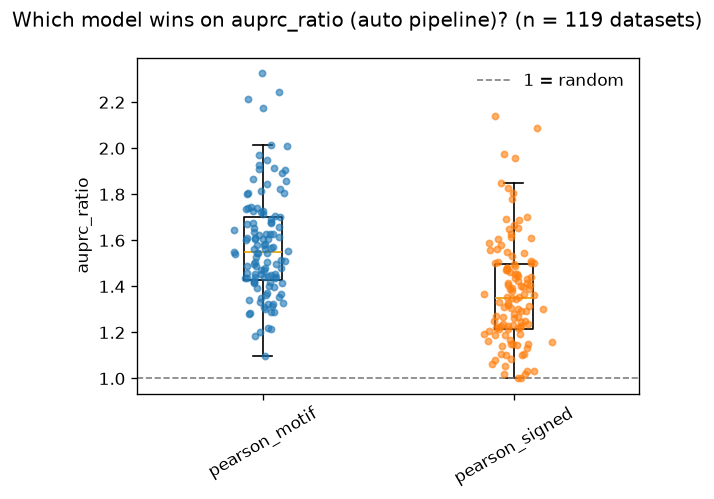
\includegraphics[width=0.85\linewidth]{../viz/scores_auprc_ratio_auto.png}
\caption{-   (n = 119 datasets) - built from  rows/ .json (auto/auprc\_ratio)}
\end{figure}
\begin{figure}[H]\centering
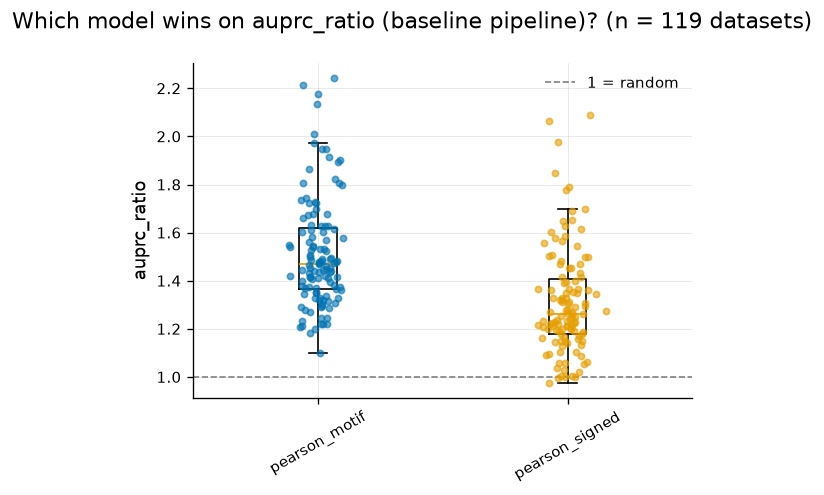
\includegraphics[width=0.85\linewidth]{../viz/scores_auprc_ratio_baseline.png}
\caption{-   (n = 119 datasets) - built from  rows/ .json (baseline/auprc\_ratio)}
\end{figure}
\begin{figure}[H]\centering
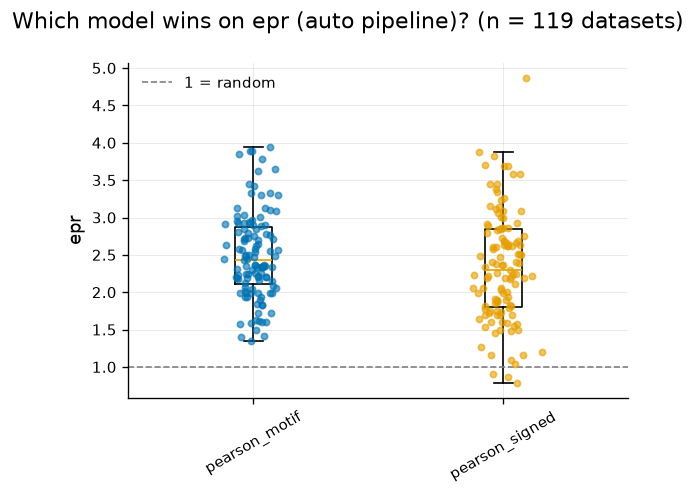
\includegraphics[width=0.85\linewidth]{../viz/scores_epr_auto.png}
\caption{-   (n = 119 datasets) - built from  rows/ .json (auto/epr)}
\end{figure}
\begin{figure}[H]\centering
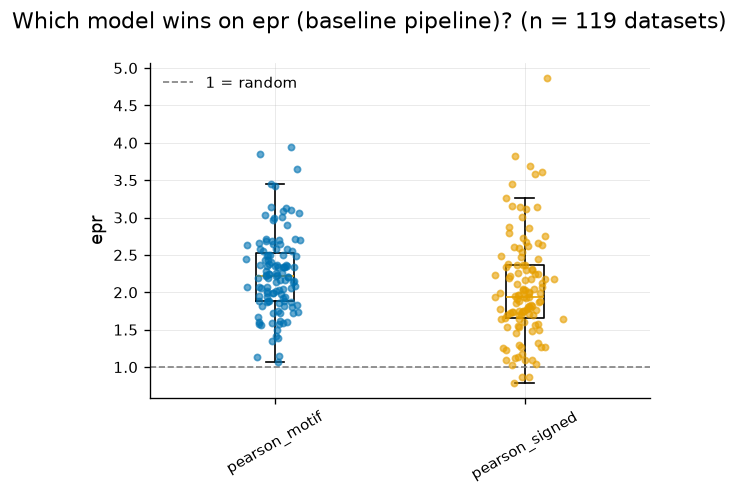
\includegraphics[width=0.85\linewidth]{../viz/scores_epr_baseline.png}
\caption{-   (n = 119 datasets) - built from  rows/ .json (baseline/epr)}
\end{figure}
\begin{figure}[H]\centering
\includegraphics[width=0.85\linewidth]{../viz/stability_cxg__10x-3-v2__homo-sapiens__brain__dc30c3ec_pearson_motif.png}
\caption{-   (n = 4 edge lists) - built from  artifacts/cxg\_\_10x-3-v2\_\_homo-sapiens\_\_brain\_\_dc30c3ec/auto/ /pearson\_motif.tsv.gz}
\end{figure}
\begin{figure}[H]\centering
\includegraphics[width=0.85\linewidth]{../viz/stability_cxg__10x-3-v2__homo-sapiens__brain__dc30c3ec_pearson_signed.png}
\caption{-   (n = 4 edge lists) - built from  artifacts/cxg\_\_10x-3-v2\_\_homo-sapiens\_\_brain\_\_dc30c3ec/auto/ /pearson\_signed.tsv.gz}
\end{figure}
\begin{figure}[H]\centering
\includegraphics[width=0.85\linewidth]{../viz/stability_cxg__10x-3-v2__homo-sapiens__breast__9a64bf99_pearson_motif.png}
\caption{-   (n = 4 edge lists) - built from  artifacts/cxg\_\_10x-3-v2\_\_homo-sapiens\_\_breast\_\_9a64bf99/auto/ /pearson\_motif.tsv.gz}
\end{figure}
\begin{figure}[H]\centering
\includegraphics[width=0.85\linewidth]{../viz/stability_cxg__10x-3-v2__homo-sapiens__breast__9a64bf99_pearson_signed.png}
\caption{-   (n = 4 edge lists) - built from  artifacts/cxg\_\_10x-3-v2\_\_homo-sapiens\_\_breast\_\_9a64bf99/auto/ /pearson\_signed.tsv.gz}
\end{figure}
\begin{figure}[H]\centering
\includegraphics[width=0.85\linewidth]{../viz/stability_cxg__10x-3-v2__homo-sapiens__fovea-centralis__babbf9f3_pearson_motif.png}
\caption{-   (n = 4 edge lists) - built from  artifacts/cxg\_\_10x-3-v2\_\_homo-sapiens\_\_fovea-centralis\_\_babbf9f3/auto/ /pearson\_motif.tsv.gz}
\end{figure}
\begin{figure}[H]\centering
\includegraphics[width=0.85\linewidth]{../viz/stability_cxg__10x-3-v2__homo-sapiens__fovea-centralis__babbf9f3_pearson_signed.png}
\caption{-   (n = 4 edge lists) - built from  artifacts/cxg\_\_10x-3-v2\_\_homo-sapiens\_\_fovea-centralis\_\_babbf9f3/auto/ /pearson\_signed.tsv.gz}
\end{figure}
\begin{figure}[H]\centering
\includegraphics[width=0.85\linewidth]{../viz/stability_cxg__10x-3-v2__homo-sapiens__thymus__11ff73e8_pearson_motif.png}
\caption{-   (n = 4 edge lists) - built from  artifacts/cxg\_\_10x-3-v2\_\_homo-sapiens\_\_thymus\_\_11ff73e8/auto/ /pearson\_motif.tsv.gz}
\end{figure}
\begin{figure}[H]\centering
\includegraphics[width=0.85\linewidth]{../viz/stability_cxg__10x-3-v2__homo-sapiens__thymus__11ff73e8_pearson_signed.png}
\caption{-   (n = 4 edge lists) - built from  artifacts/cxg\_\_10x-3-v2\_\_homo-sapiens\_\_thymus\_\_11ff73e8/auto/ /pearson\_signed.tsv.gz}
\end{figure}
\begin{figure}[H]\centering
\includegraphics[width=0.85\linewidth]{../viz/stability_cxg__10x-3-v3__homo-sapiens__apex-of-heart__2e9d2f32_pearson_motif.png}
\caption{-   (n = 4 edge lists) - built from  artifacts/cxg\_\_10x-3-v3\_\_homo-sapiens\_\_apex-of-heart\_\_2e9d2f32/auto/ /pearson\_motif.tsv.gz}
\end{figure}
\begin{figure}[H]\centering
\includegraphics[width=0.85\linewidth]{../viz/stability_cxg__10x-3-v3__homo-sapiens__apex-of-heart__2e9d2f32_pearson_signed.png}
\caption{-   (n = 4 edge lists) - built from  artifacts/cxg\_\_10x-3-v3\_\_homo-sapiens\_\_apex-of-heart\_\_2e9d2f32/auto/ /pearson\_signed.tsv.gz}
\end{figure}
\begin{figure}[H]\centering
\includegraphics[width=0.85\linewidth]{../viz/stability_cxg__10x-3-v3__homo-sapiens__blood__738942eb_pearson_motif.png}
\caption{-   (n = 4 edge lists) - built from  artifacts/cxg\_\_10x-3-v3\_\_homo-sapiens\_\_blood\_\_738942eb/auto/ /pearson\_motif.tsv.gz}
\end{figure}
\begin{figure}[H]\centering
\includegraphics[width=0.85\linewidth]{../viz/stability_cxg__10x-3-v3__homo-sapiens__blood__738942eb_pearson_signed.png}
\caption{-   (n = 4 edge lists) - built from  artifacts/cxg\_\_10x-3-v3\_\_homo-sapiens\_\_blood\_\_738942eb/auto/ /pearson\_signed.tsv.gz}
\end{figure}
\begin{figure}[H]\centering
\includegraphics[width=0.85\linewidth]{../viz/stability_cxg__10x-3-v3__homo-sapiens__caudate-nucleus__c893ddc3_pearson_motif.png}
\caption{-   (n = 4 edge lists) - built from  artifacts/cxg\_\_10x-3-v3\_\_homo-sapiens\_\_caudate-nucleus\_\_c893ddc3/auto/ /pearson\_motif.tsv.gz}
\end{figure}
\begin{figure}[H]\centering
\includegraphics[width=0.85\linewidth]{../viz/stability_cxg__10x-3-v3__homo-sapiens__caudate-nucleus__c893ddc3_pearson_signed.png}
\caption{-   (n = 4 edge lists) - built from  artifacts/cxg\_\_10x-3-v3\_\_homo-sapiens\_\_caudate-nucleus\_\_c893ddc3/auto/ /pearson\_signed.tsv.gz}
\end{figure}
\begin{figure}[H]\centering
\includegraphics[width=0.85\linewidth]{../viz/stability_cxg__10x-3-v3__homo-sapiens__cornea__8058d760_pearson_motif.png}
\caption{-   (n = 4 edge lists) - built from  artifacts/cxg\_\_10x-3-v3\_\_homo-sapiens\_\_cornea\_\_8058d760/auto/ /pearson\_motif.tsv.gz}
\end{figure}
\begin{figure}[H]\centering
\includegraphics[width=0.85\linewidth]{../viz/stability_cxg__10x-3-v3__homo-sapiens__cornea__8058d760_pearson_signed.png}
\caption{-   (n = 4 edge lists) - built from  artifacts/cxg\_\_10x-3-v3\_\_homo-sapiens\_\_cornea\_\_8058d760/auto/ /pearson\_signed.tsv.gz}
\end{figure}
\begin{figure}[H]\centering
\includegraphics[width=0.85\linewidth]{../viz/stability_cxg__10x-3-v3__homo-sapiens__cranial-nerve-ii__9f1a899f_pearson_motif.png}
\caption{-   (n = 4 edge lists) - built from  artifacts/cxg\_\_10x-3-v3\_\_homo-sapiens\_\_cranial-nerve-ii\_\_9f1a899f/auto/ /pearson\_motif.tsv.gz}
\end{figure}
\begin{figure}[H]\centering
\includegraphics[width=0.85\linewidth]{../viz/stability_cxg__10x-3-v3__homo-sapiens__cranial-nerve-ii__9f1a899f_pearson_signed.png}
\caption{-   (n = 4 edge lists) - built from  artifacts/cxg\_\_10x-3-v3\_\_homo-sapiens\_\_cranial-nerve-ii\_\_9f1a899f/auto/ /pearson\_signed.tsv.gz}
\end{figure}
\begin{figure}[H]\centering
\includegraphics[width=0.85\linewidth]{../viz/stability_cxg__10x-3-v3__homo-sapiens__entorhinal-cortex__24584be9_pearson_motif.png}
\caption{-   (n = 4 edge lists) - built from  artifacts/cxg\_\_10x-3-v3\_\_homo-sapiens\_\_entorhinal-cortex\_\_24584be9/auto/ /pearson\_motif.tsv.gz}
\end{figure}
\begin{figure}[H]\centering
\includegraphics[width=0.85\linewidth]{../viz/stability_cxg__10x-3-v3__homo-sapiens__entorhinal-cortex__24584be9_pearson_signed.png}
\caption{-   (n = 4 edge lists) - built from  artifacts/cxg\_\_10x-3-v3\_\_homo-sapiens\_\_entorhinal-cortex\_\_24584be9/auto/ /pearson\_signed.tsv.gz}
\end{figure}
\begin{figure}[H]\centering
\includegraphics[width=0.85\linewidth]{../viz/stability_cxg__10x-3-v3__homo-sapiens__fovea-centralis__e404d417_pearson_motif.png}
\caption{-   (n = 3 edge lists) - built from  artifacts/cxg\_\_10x-3-v3\_\_homo-sapiens\_\_fovea-centralis\_\_e404d417/auto/ /pearson\_motif.tsv.gz}
\end{figure}
\begin{figure}[H]\centering
\includegraphics[width=0.85\linewidth]{../viz/stability_cxg__10x-3-v3__homo-sapiens__fovea-centralis__e404d417_pearson_signed.png}
\caption{-   (n = 3 edge lists) - built from  artifacts/cxg\_\_10x-3-v3\_\_homo-sapiens\_\_fovea-centralis\_\_e404d417/auto/ /pearson\_signed.tsv.gz}
\end{figure}
\begin{figure}[H]\centering
\includegraphics[width=0.85\linewidth]{../viz/stability_cxg__10x-3-v3__homo-sapiens__heart-left-ventricle__f15e263b_pearson_motif.png}
\caption{-   (n = 4 edge lists) - built from  artifacts/cxg\_\_10x-3-v3\_\_homo-sapiens\_\_heart-left-ventricle\_\_f15e263b/auto/ /pearson\_motif.tsv.gz}
\end{figure}
\begin{figure}[H]\centering
\includegraphics[width=0.85\linewidth]{../viz/stability_cxg__10x-3-v3__homo-sapiens__heart-left-ventricle__f15e263b_pearson_signed.png}
\caption{-   (n = 4 edge lists) - built from  artifacts/cxg\_\_10x-3-v3\_\_homo-sapiens\_\_heart-left-ventricle\_\_f15e263b/auto/ /pearson\_signed.tsv.gz}
\end{figure}
\begin{figure}[H]\centering
\includegraphics[width=0.85\linewidth]{../viz/stability_cxg__10x-3-v3__homo-sapiens__left-atrium-auricular-region__87a06a2a_pearson_motif.png}
\caption{-   (n = 4 edge lists) - built from  artifacts/cxg\_\_10x-3-v3\_\_homo-sapiens\_\_left-atrium-auricular-region\_\_87a06a2a/auto/ /pearson\_motif.tsv.gz}
\end{figure}
\begin{figure}[H]\centering
\includegraphics[width=0.85\linewidth]{../viz/stability_cxg__10x-3-v3__homo-sapiens__left-atrium-auricular-region__87a06a2a_pearson_signed.png}
\caption{-   (n = 4 edge lists) - built from  artifacts/cxg\_\_10x-3-v3\_\_homo-sapiens\_\_left-atrium-auricular-region\_\_87a06a2a/auto/ /pearson\_signed.tsv.gz}
\end{figure}
\begin{figure}[H]\centering
\includegraphics[width=0.85\linewidth]{../viz/stability_cxg__10x-3-v3__homo-sapiens__mesenteric-artery__42b6a476_pearson_motif.png}
\caption{-   (n = 2 edge lists) - built from  artifacts/cxg\_\_10x-3-v3\_\_homo-sapiens\_\_mesenteric-artery\_\_42b6a476/auto/ /pearson\_motif.tsv.gz}
\end{figure}
\begin{figure}[H]\centering
\includegraphics[width=0.85\linewidth]{../viz/stability_cxg__10x-3-v3__homo-sapiens__mesenteric-artery__42b6a476_pearson_signed.png}
\caption{-   (n = 2 edge lists) - built from  artifacts/cxg\_\_10x-3-v3\_\_homo-sapiens\_\_mesenteric-artery\_\_42b6a476/auto/ /pearson\_signed.tsv.gz}
\end{figure}
\begin{figure}[H]\centering
\includegraphics[width=0.85\linewidth]{../viz/stability_cxg__10x-3-v3__homo-sapiens__occipital-cortex__e6361237_pearson_motif.png}
\caption{-   (n = 4 edge lists) - built from  artifacts/cxg\_\_10x-3-v3\_\_homo-sapiens\_\_occipital-cortex\_\_e6361237/auto/ /pearson\_motif.tsv.gz}
\end{figure}
\begin{figure}[H]\centering
\includegraphics[width=0.85\linewidth]{../viz/stability_cxg__10x-3-v3__homo-sapiens__occipital-cortex__e6361237_pearson_signed.png}
\caption{-   (n = 4 edge lists) - built from  artifacts/cxg\_\_10x-3-v3\_\_homo-sapiens\_\_occipital-cortex\_\_e6361237/auto/ /pearson\_signed.tsv.gz}
\end{figure}
\begin{figure}[H]\centering
\includegraphics[width=0.85\linewidth]{../viz/stability_cxg__10x-3-v3__homo-sapiens__skin-of-body__b796f27e_pearson_motif.png}
\caption{-   (n = 4 edge lists) - built from  artifacts/cxg\_\_10x-3-v3\_\_homo-sapiens\_\_skin-of-body\_\_b796f27e/auto/ /pearson\_motif.tsv.gz}
\end{figure}
\begin{figure}[H]\centering
\includegraphics[width=0.85\linewidth]{../viz/stability_cxg__10x-3-v3__homo-sapiens__skin-of-body__b796f27e_pearson_signed.png}
\caption{-   (n = 4 edge lists) - built from  artifacts/cxg\_\_10x-3-v3\_\_homo-sapiens\_\_skin-of-body\_\_b796f27e/auto/ /pearson\_signed.tsv.gz}
\end{figure}
\begin{figure}[H]\centering
\includegraphics[width=0.85\linewidth]{../viz/stability_cxg__10x-3-v3__mus-musculus__brain__e056b20b_pearson_motif.png}
\caption{-   (n = 4 edge lists) - built from  artifacts/cxg\_\_10x-3-v3\_\_mus-musculus\_\_brain\_\_e056b20b/auto/ /pearson\_motif.tsv.gz}
\end{figure}
\begin{figure}[H]\centering
\includegraphics[width=0.85\linewidth]{../viz/stability_cxg__10x-3-v3__mus-musculus__brain__e056b20b_pearson_signed.png}
\caption{-   (n = 4 edge lists) - built from  artifacts/cxg\_\_10x-3-v3\_\_mus-musculus\_\_brain\_\_e056b20b/auto/ /pearson\_signed.tsv.gz}
\end{figure}
\begin{figure}[H]\centering
\includegraphics[width=0.85\linewidth]{../viz/stability_cxg__10x-3-v3__mus-musculus__middle-lobe-of-right-lung__89840cec_pearson_motif.png}
\caption{-   (n = 4 edge lists) - built from  artifacts/cxg\_\_10x-3-v3\_\_mus-musculus\_\_middle-lobe-of-right-lung\_\_89840cec/auto/ /pearson\_motif.tsv.gz}
\end{figure}
\begin{figure}[H]\centering
\includegraphics[width=0.85\linewidth]{../viz/stability_cxg__10x-3-v3__mus-musculus__middle-lobe-of-right-lung__89840cec_pearson_signed.png}
\caption{-   (n = 4 edge lists) - built from  artifacts/cxg\_\_10x-3-v3\_\_mus-musculus\_\_middle-lobe-of-right-lung\_\_89840cec/auto/ /pearson\_signed.tsv.gz}
\end{figure}
\begin{figure}[H]\centering
\includegraphics[width=0.85\linewidth]{../viz/stability_cxg__10x-5-transcription-profiling__homo-sapiens__adrenal-tissue__5af90777_pearson_motif.png}
\caption{-   (n = 4 edge lists) - built from  artifacts/cxg\_\_10x-5-transcription-profiling\_\_homo-sapiens\_\_adrenal-tissue\_\_5af90777/auto/ /pearson\_motif.tsv.gz}
\end{figure}
\begin{figure}[H]\centering
\includegraphics[width=0.85\linewidth]{../viz/stability_cxg__10x-5-transcription-profiling__homo-sapiens__adrenal-tissue__5af90777_pearson_signed.png}
\caption{-   (n = 4 edge lists) - built from  artifacts/cxg\_\_10x-5-transcription-profiling\_\_homo-sapiens\_\_adrenal-tissue\_\_5af90777/auto/ /pearson\_signed.tsv.gz}
\end{figure}
\begin{figure}[H]\centering
\includegraphics[width=0.85\linewidth]{../viz/stability_cxg__10x-5-v1__homo-sapiens__lymph-node__99950e99_pearson_motif.png}
\caption{-   (n = 4 edge lists) - built from  artifacts/cxg\_\_10x-5-v1\_\_homo-sapiens\_\_lymph-node\_\_99950e99/auto/ /pearson\_motif.tsv.gz}
\end{figure}
\begin{figure}[H]\centering
\includegraphics[width=0.85\linewidth]{../viz/stability_cxg__10x-5-v1__homo-sapiens__lymph-node__99950e99_pearson_signed.png}
\caption{-   (n = 4 edge lists) - built from  artifacts/cxg\_\_10x-5-v1\_\_homo-sapiens\_\_lymph-node\_\_99950e99/auto/ /pearson\_signed.tsv.gz}
\end{figure}
\begin{figure}[H]\centering
\includegraphics[width=0.85\linewidth]{../viz/stability_cxg__10x-5-v1__homo-sapiens__t-cell__0c774045_pearson_motif.png}
\caption{-   (n = 4 edge lists) - built from  artifacts/cxg\_\_10x-5-v1\_\_homo-sapiens\_\_t-cell\_\_0c774045/auto/ /pearson\_motif.tsv.gz}
\end{figure}
\begin{figure}[H]\centering
\includegraphics[width=0.85\linewidth]{../viz/stability_cxg__10x-5-v1__homo-sapiens__t-cell__0c774045_pearson_signed.png}
\caption{-   (n = 4 edge lists) - built from  artifacts/cxg\_\_10x-5-v1\_\_homo-sapiens\_\_t-cell\_\_0c774045/auto/ /pearson\_signed.tsv.gz}
\end{figure}
\begin{figure}[H]\centering
\includegraphics[width=0.85\linewidth]{../viz/stability_cxg__10x-5-v2__homo-sapiens__blood__bd65a70f_pearson_motif.png}
\caption{-   (n = 4 edge lists) - built from  artifacts/cxg\_\_10x-5-v2\_\_homo-sapiens\_\_blood\_\_bd65a70f/auto/ /pearson\_motif.tsv.gz}
\end{figure}
\begin{figure}[H]\centering
\includegraphics[width=0.85\linewidth]{../viz/stability_cxg__10x-5-v2__homo-sapiens__blood__bd65a70f_pearson_signed.png}
\caption{-   (n = 4 edge lists) - built from  artifacts/cxg\_\_10x-5-v2\_\_homo-sapiens\_\_blood\_\_bd65a70f/auto/ /pearson\_signed.tsv.gz}
\end{figure}
\begin{figure}[H]\centering
\includegraphics[width=0.85\linewidth]{../viz/stability_cxg__10x-multiome__homo-sapiens__amygdala__835fa5c4_pearson_motif.png}
\caption{-   (n = 4 edge lists) - built from  artifacts/cxg\_\_10x-multiome\_\_homo-sapiens\_\_amygdala\_\_835fa5c4/auto/ /pearson\_motif.tsv.gz}
\end{figure}
\begin{figure}[H]\centering
\includegraphics[width=0.85\linewidth]{../viz/stability_cxg__10x-multiome__homo-sapiens__amygdala__835fa5c4_pearson_signed.png}
\caption{-   (n = 4 edge lists) - built from  artifacts/cxg\_\_10x-multiome\_\_homo-sapiens\_\_amygdala\_\_835fa5c4/auto/ /pearson\_signed.tsv.gz}
\end{figure}
\begin{figure}[H]\centering
\includegraphics[width=0.85\linewidth]{../viz/stability_cxg__10x-multiome__homo-sapiens__anterior-cingulate-cortex__56a4bc14_pearson_motif.png}
\caption{-   (n = 4 edge lists) - built from  artifacts/cxg\_\_10x-multiome\_\_homo-sapiens\_\_anterior-cingulate-cortex\_\_56a4bc14/auto/ /pearson\_motif.tsv.gz}
\end{figure}
\begin{figure}[H]\centering
\includegraphics[width=0.85\linewidth]{../viz/stability_cxg__10x-multiome__homo-sapiens__anterior-cingulate-cortex__56a4bc14_pearson_signed.png}
\caption{-   (n = 4 edge lists) - built from  artifacts/cxg\_\_10x-multiome\_\_homo-sapiens\_\_anterior-cingulate-cortex\_\_56a4bc14/auto/ /pearson\_signed.tsv.gz}
\end{figure}
\begin{figure}[H]\centering
\includegraphics[width=0.85\linewidth]{../viz/stability_cxg__seq-well__homo-sapiens__blood__456e8b9b_pearson_motif.png}
\caption{-   (n = 4 edge lists) - built from  artifacts/cxg\_\_seq-well\_\_homo-sapiens\_\_blood\_\_456e8b9b/auto/ /pearson\_motif.tsv.gz}
\end{figure}
\begin{figure}[H]\centering
\includegraphics[width=0.85\linewidth]{../viz/stability_cxg__seq-well__homo-sapiens__blood__456e8b9b_pearson_signed.png}
\caption{-   (n = 4 edge lists) - built from  artifacts/cxg\_\_seq-well\_\_homo-sapiens\_\_blood\_\_456e8b9b/auto/ /pearson\_signed.tsv.gz}
\end{figure}
\begin{figure}[H]\centering
\includegraphics[width=0.85\linewidth]{../viz/stability_cxg__smart-seq-v4__mus-musculus__primary-motor-cortex__1304e107_pearson_motif.png}
\caption{-   (n = 2 edge lists) - built from  artifacts/cxg\_\_smart-seq-v4\_\_mus-musculus\_\_primary-motor-cortex\_\_1304e107/auto/ /pearson\_motif.tsv.gz}
\end{figure}
\begin{figure}[H]\centering
\includegraphics[width=0.85\linewidth]{../viz/stability_cxg__smart-seq-v4__mus-musculus__primary-motor-cortex__1304e107_pearson_signed.png}
\caption{-   (n = 2 edge lists) - built from  artifacts/cxg\_\_smart-seq-v4\_\_mus-musculus\_\_primary-motor-cortex\_\_1304e107/auto/ /pearson\_signed.tsv.gz}
\end{figure}
\begin{figure}[H]\centering
\includegraphics[width=0.85\linewidth]{../viz/stability_cxg__smart-seq__mus-musculus__primary-visual-cortex__3a15ab1c_pearson_motif.png}
\caption{-   (n = 2 edge lists) - built from  artifacts/cxg\_\_smart-seq\_\_mus-musculus\_\_primary-visual-cortex\_\_3a15ab1c/auto/ /pearson\_motif.tsv.gz}
\end{figure}
\begin{figure}[H]\centering
\includegraphics[width=0.85\linewidth]{../viz/stability_cxg__smart-seq__mus-musculus__primary-visual-cortex__3a15ab1c_pearson_signed.png}
\caption{-   (n = 2 edge lists) - built from  artifacts/cxg\_\_smart-seq\_\_mus-musculus\_\_primary-visual-cortex\_\_3a15ab1c/auto/ /pearson\_signed.tsv.gz}
\end{figure}
\begin{figure}[H]\centering
\includegraphics[width=0.85\linewidth]{../viz/tf_recovery_cxg__10x-3-v2__homo-sapiens__anterior-wall-of-left-ventricl__4ed927e9.png}
\caption{-   (n = up to 30 TFs) - built from  artifacts/cxg\_\_10x-3-v2\_\_homo-sapiens\_\_anterior-wall-of-left-ventricl\_\_4ed927e9/auto}
\end{figure}
\begin{figure}[H]\centering
\includegraphics[width=0.85\linewidth]{../viz/tf_recovery_cxg__10x-3-v2__homo-sapiens__blood__ae5341b8.png}
\caption{-   (n = up to 30 TFs) - built from  artifacts/cxg\_\_10x-3-v2\_\_homo-sapiens\_\_blood\_\_ae5341b8/auto}
\end{figure}
\begin{figure}[H]\centering
\includegraphics[width=0.85\linewidth]{../viz/tf_recovery_cxg__10x-3-v2__homo-sapiens__brain__dc30c3ec.png}
\caption{-   (n = up to 30 TFs) - built from  artifacts/cxg\_\_10x-3-v2\_\_homo-sapiens\_\_brain\_\_dc30c3ec/auto}
\end{figure}
\begin{figure}[H]\centering
\includegraphics[width=0.85\linewidth]{../viz/tf_recovery_cxg__10x-3-v2__homo-sapiens__breast__9a64bf99.png}
\caption{-   (n = up to 30 TFs) - built from  artifacts/cxg\_\_10x-3-v2\_\_homo-sapiens\_\_breast\_\_9a64bf99/auto}
\end{figure}
\begin{figure}[H]\centering
\includegraphics[width=0.85\linewidth]{../viz/tf_recovery_cxg__10x-3-v2__homo-sapiens__caudate-lobe-of-liver__a43aa46b.png}
\caption{-   (n = up to 30 TFs) - built from  artifacts/cxg\_\_10x-3-v2\_\_homo-sapiens\_\_caudate-lobe-of-liver\_\_a43aa46b/auto}
\end{figure}
\begin{figure}[H]\centering
\includegraphics[width=0.85\linewidth]{../viz/tf_recovery_cxg__10x-3-v2__homo-sapiens__cortex-of-kidney__105c7dad.png}
\caption{-   (n = up to 30 TFs) - built from  artifacts/cxg\_\_10x-3-v2\_\_homo-sapiens\_\_cortex-of-kidney\_\_105c7dad/auto}
\end{figure}
\begin{figure}[H]\centering
\includegraphics[width=0.85\linewidth]{../viz/tf_recovery_cxg__10x-3-v2__homo-sapiens__dental-pulp__bdd109f1.png}
\caption{-   (n = up to 30 TFs) - built from  artifacts/cxg\_\_10x-3-v2\_\_homo-sapiens\_\_dental-pulp\_\_bdd109f1/auto}
\end{figure}
\begin{figure}[H]\centering
\includegraphics[width=0.85\linewidth]{../viz/tf_recovery_cxg__10x-3-v2__homo-sapiens__epithelium-of-rectum__80d7111d.png}
\caption{-   (n = up to 30 TFs) - built from  artifacts/cxg\_\_10x-3-v2\_\_homo-sapiens\_\_epithelium-of-rectum\_\_80d7111d/auto}
\end{figure}
\begin{figure}[H]\centering
\includegraphics[width=0.85\linewidth]{../viz/tf_recovery_cxg__10x-3-v2__homo-sapiens__fovea-centralis__babbf9f3.png}
\caption{-   (n = up to 30 TFs) - built from  artifacts/cxg\_\_10x-3-v2\_\_homo-sapiens\_\_fovea-centralis\_\_babbf9f3/auto}
\end{figure}
\begin{figure}[H]\centering
\includegraphics[width=0.85\linewidth]{../viz/tf_recovery_cxg__10x-3-v2__homo-sapiens__kidney__8dc29642.png}
\caption{-   (n = up to 30 TFs) - built from  artifacts/cxg\_\_10x-3-v2\_\_homo-sapiens\_\_kidney\_\_8dc29642/auto}
\end{figure}
\begin{figure}[H]\centering
\includegraphics[width=0.85\linewidth]{../viz/tf_recovery_cxg__10x-3-v2__homo-sapiens__lung__6e00ccf7.png}
\caption{-   (n = up to 30 TFs) - built from  artifacts/cxg\_\_10x-3-v2\_\_homo-sapiens\_\_lung\_\_6e00ccf7/auto}
\end{figure}
\begin{figure}[H]\centering
\includegraphics[width=0.85\linewidth]{../viz/tf_recovery_cxg__10x-3-v2__homo-sapiens__mammary-gland-connective-tissu__68b6114f.png}
\caption{-   (n = up to 30 TFs) - built from  artifacts/cxg\_\_10x-3-v2\_\_homo-sapiens\_\_mammary-gland-connective-tissu\_\_68b6114f/auto}
\end{figure}
\begin{figure}[H]\centering
\includegraphics[width=0.85\linewidth]{../viz/tf_recovery_cxg__10x-3-v2__homo-sapiens__ovary__1f1c5c14.png}
\caption{-   (n = up to 30 TFs) - built from  artifacts/cxg\_\_10x-3-v2\_\_homo-sapiens\_\_ovary\_\_1f1c5c14/auto}
\end{figure}
\begin{figure}[H]\centering
\includegraphics[width=0.85\linewidth]{../viz/tf_recovery_cxg__10x-3-v2__homo-sapiens__respiratory-airway__8fcf0ccc.png}
\caption{-   (n = up to 30 TFs) - built from  artifacts/cxg\_\_10x-3-v2\_\_homo-sapiens\_\_respiratory-airway\_\_8fcf0ccc/auto}
\end{figure}
\begin{figure}[H]\centering
\includegraphics[width=0.85\linewidth]{../viz/tf_recovery_cxg__10x-3-v2__homo-sapiens__skin-of-prepuce-of-penis__f512b8b6.png}
\caption{-   (n = up to 30 TFs) - built from  artifacts/cxg\_\_10x-3-v2\_\_homo-sapiens\_\_skin-of-prepuce-of-penis\_\_f512b8b6/auto}
\end{figure}
\begin{figure}[H]\centering
\includegraphics[width=0.85\linewidth]{../viz/tf_recovery_cxg__10x-3-v2__homo-sapiens__thymus__11ff73e8.png}
\caption{-   (n = up to 30 TFs) - built from  artifacts/cxg\_\_10x-3-v2\_\_homo-sapiens\_\_thymus\_\_11ff73e8/auto}
\end{figure}
\begin{figure}[H]\centering
\includegraphics[width=0.85\linewidth]{../viz/tf_recovery_cxg__10x-3-v2__homo-sapiens__zone-of-skin__124744b8.png}
\caption{-   (n = up to 30 TFs) - built from  artifacts/cxg\_\_10x-3-v2\_\_homo-sapiens\_\_zone-of-skin\_\_124744b8/auto}
\end{figure}
\begin{figure}[H]\centering
\includegraphics[width=0.85\linewidth]{../viz/tf_recovery_cxg__10x-3-v2__mus-musculus__hindlimb-muscle__bedee313.png}
\caption{-   (n = up to 30 TFs) - built from  artifacts/cxg\_\_10x-3-v2\_\_mus-musculus\_\_hindlimb-muscle\_\_bedee313/auto}
\end{figure}
\begin{figure}[H]\centering
\includegraphics[width=0.85\linewidth]{../viz/tf_recovery_cxg__10x-3-v3__homo-sapiens__abdomen__7b95971d.png}
\caption{-   (n = up to 30 TFs) - built from  artifacts/cxg\_\_10x-3-v3\_\_homo-sapiens\_\_abdomen\_\_7b95971d/auto}
\end{figure}
\begin{figure}[H]\centering
\includegraphics[width=0.85\linewidth]{../viz/tf_recovery_cxg__10x-3-v3__homo-sapiens__abdomen__97d9238c.png}
\caption{-   (n = up to 30 TFs) - built from  artifacts/cxg\_\_10x-3-v3\_\_homo-sapiens\_\_abdomen\_\_97d9238c/auto}
\end{figure}
\begin{figure}[H]\centering
\includegraphics[width=0.85\linewidth]{../viz/tf_recovery_cxg__10x-3-v3__homo-sapiens__apex-of-heart__2e9d2f32.png}
\caption{-   (n = up to 30 TFs) - built from  artifacts/cxg\_\_10x-3-v3\_\_homo-sapiens\_\_apex-of-heart\_\_2e9d2f32/auto}
\end{figure}
\begin{figure}[H]\centering
\includegraphics[width=0.85\linewidth]{../viz/tf_recovery_cxg__10x-3-v3__homo-sapiens__blood__19e46756.png}
\caption{-   (n = up to 30 TFs) - built from  artifacts/cxg\_\_10x-3-v3\_\_homo-sapiens\_\_blood\_\_19e46756/auto}
\end{figure}
\begin{figure}[H]\centering
\includegraphics[width=0.85\linewidth]{../viz/tf_recovery_cxg__10x-3-v3__homo-sapiens__blood__20fae564.png}
\caption{-   (n = up to 30 TFs) - built from  artifacts/cxg\_\_10x-3-v3\_\_homo-sapiens\_\_blood\_\_20fae564/auto}
\end{figure}
\begin{figure}[H]\centering
\includegraphics[width=0.85\linewidth]{../viz/tf_recovery_cxg__10x-3-v3__homo-sapiens__blood__738942eb.png}
\caption{-   (n = up to 30 TFs) - built from  artifacts/cxg\_\_10x-3-v3\_\_homo-sapiens\_\_blood\_\_738942eb/auto}
\end{figure}
\begin{figure}[H]\centering
\includegraphics[width=0.85\linewidth]{../viz/tf_recovery_cxg__10x-3-v3__homo-sapiens__blood__a199ca73.png}
\caption{-   (n = up to 30 TFs) - built from  artifacts/cxg\_\_10x-3-v3\_\_homo-sapiens\_\_blood\_\_a199ca73/auto}
\end{figure}
\begin{figure}[H]\centering
\includegraphics[width=0.85\linewidth]{../viz/tf_recovery_cxg__10x-3-v3__homo-sapiens__blood__d9f3a82c.png}
\caption{-   (n = up to 30 TFs) - built from  artifacts/cxg\_\_10x-3-v3\_\_homo-sapiens\_\_blood\_\_d9f3a82c/auto}
\end{figure}
\begin{figure}[H]\centering
\includegraphics[width=0.85\linewidth]{../viz/tf_recovery_cxg__10x-3-v3__homo-sapiens__blood__de2c780c.png}
\caption{-   (n = up to 30 TFs) - built from  artifacts/cxg\_\_10x-3-v3\_\_homo-sapiens\_\_blood\_\_de2c780c/auto}
\end{figure}
\begin{figure}[H]\centering
\includegraphics[width=0.85\linewidth]{../viz/tf_recovery_cxg__10x-3-v3__homo-sapiens__bone-marrow__343ff97c.png}
\caption{-   (n = up to 30 TFs) - built from  artifacts/cxg\_\_10x-3-v3\_\_homo-sapiens\_\_bone-marrow\_\_343ff97c/auto}
\end{figure}
\begin{figure}[H]\centering
\includegraphics[width=0.85\linewidth]{../viz/tf_recovery_cxg__10x-3-v3__homo-sapiens__breast__24ec2dc5.png}
\caption{-   (n = up to 30 TFs) - built from  artifacts/cxg\_\_10x-3-v3\_\_homo-sapiens\_\_breast\_\_24ec2dc5/auto}
\end{figure}
\begin{figure}[H]\centering
\includegraphics[width=0.85\linewidth]{../viz/tf_recovery_cxg__10x-3-v3__homo-sapiens__brodmann-1909-area-13__f16f4108.png}
\caption{-   (n = up to 30 TFs) - built from  artifacts/cxg\_\_10x-3-v3\_\_homo-sapiens\_\_brodmann-1909-area-13\_\_f16f4108/auto}
\end{figure}
\begin{figure}[H]\centering
\includegraphics[width=0.85\linewidth]{../viz/tf_recovery_cxg__10x-3-v3__homo-sapiens__brodmann-1909-area-4__c8f83821.png}
\caption{-   (n = up to 30 TFs) - built from  artifacts/cxg\_\_10x-3-v3\_\_homo-sapiens\_\_brodmann-1909-area-4\_\_c8f83821/auto}
\end{figure}
\begin{figure}[H]\centering
\includegraphics[width=0.85\linewidth]{../viz/tf_recovery_cxg__10x-3-v3__homo-sapiens__brown-preadipocyte__137ca42b.png}
\caption{-   (n = up to 30 TFs) - built from  artifacts/cxg\_\_10x-3-v3\_\_homo-sapiens\_\_brown-preadipocyte\_\_137ca42b/auto}
\end{figure}
\begin{figure}[H]\centering
\includegraphics[width=0.85\linewidth]{../viz/tf_recovery_cxg__10x-3-v3__homo-sapiens__calcaneal-tendon__ef0fc6ac.png}
\caption{-   (n = up to 30 TFs) - built from  artifacts/cxg\_\_10x-3-v3\_\_homo-sapiens\_\_calcaneal-tendon\_\_ef0fc6ac/auto}
\end{figure}
\begin{figure}[H]\centering
\includegraphics[width=0.85\linewidth]{../viz/tf_recovery_cxg__10x-3-v3__homo-sapiens__calcaneal-tendon__f641d68a.png}
\caption{-   (n = up to 30 TFs) - built from  artifacts/cxg\_\_10x-3-v3\_\_homo-sapiens\_\_calcaneal-tendon\_\_f641d68a/auto}
\end{figure}
\begin{figure}[H]\centering
\includegraphics[width=0.85\linewidth]{../viz/tf_recovery_cxg__10x-3-v3__homo-sapiens__caudate-nucleus__c893ddc3.png}
\caption{-   (n = up to 30 TFs) - built from  artifacts/cxg\_\_10x-3-v3\_\_homo-sapiens\_\_caudate-nucleus\_\_c893ddc3/auto}
\end{figure}
\begin{figure}[H]\centering
\includegraphics[width=0.85\linewidth]{../viz/tf_recovery_cxg__10x-3-v3__homo-sapiens__cerebellum__be884a28.png}
\caption{-   (n = up to 30 TFs) - built from  artifacts/cxg\_\_10x-3-v3\_\_homo-sapiens\_\_cerebellum\_\_be884a28/auto}
\end{figure}
\begin{figure}[H]\centering
\includegraphics[width=0.85\linewidth]{../viz/tf_recovery_cxg__10x-3-v3__homo-sapiens__cornea__8058d760.png}
\caption{-   (n = up to 30 TFs) - built from  artifacts/cxg\_\_10x-3-v3\_\_homo-sapiens\_\_cornea\_\_8058d760/auto}
\end{figure}
\begin{figure}[H]\centering
\includegraphics[width=0.85\linewidth]{../viz/tf_recovery_cxg__10x-3-v3__homo-sapiens__cortex-of-kidney__07854d9c.png}
\caption{-   (n = up to 30 TFs) - built from  artifacts/cxg\_\_10x-3-v3\_\_homo-sapiens\_\_cortex-of-kidney\_\_07854d9c/auto}
\end{figure}
\begin{figure}[H]\centering
\includegraphics[width=0.85\linewidth]{../viz/tf_recovery_cxg__10x-3-v3__homo-sapiens__cortex-of-kidney__0bae7ebf.png}
\caption{-   (n = up to 30 TFs) - built from  artifacts/cxg\_\_10x-3-v3\_\_homo-sapiens\_\_cortex-of-kidney\_\_0bae7ebf/auto}
\end{figure}
\begin{figure}[H]\centering
\includegraphics[width=0.85\linewidth]{../viz/tf_recovery_cxg__10x-3-v3__homo-sapiens__cranial-nerve-ii__374edd6c.png}
\caption{-   (n = up to 30 TFs) - built from  artifacts/cxg\_\_10x-3-v3\_\_homo-sapiens\_\_cranial-nerve-ii\_\_374edd6c/auto}
\end{figure}
\begin{figure}[H]\centering
\includegraphics[width=0.85\linewidth]{../viz/tf_recovery_cxg__10x-3-v3__homo-sapiens__cranial-nerve-ii__9f1a899f.png}
\caption{-   (n = up to 30 TFs) - built from  artifacts/cxg\_\_10x-3-v3\_\_homo-sapiens\_\_cranial-nerve-ii\_\_9f1a899f/auto}
\end{figure}
\begin{figure}[H]\centering
\includegraphics[width=0.85\linewidth]{../viz/tf_recovery_cxg__10x-3-v3__homo-sapiens__dome-of-urinary-bladder__601c7454.png}
\caption{-   (n = up to 30 TFs) - built from  artifacts/cxg\_\_10x-3-v3\_\_homo-sapiens\_\_dome-of-urinary-bladder\_\_601c7454/auto}
\end{figure}
\begin{figure}[H]\centering
\includegraphics[width=0.85\linewidth]{../viz/tf_recovery_cxg__10x-3-v3__homo-sapiens__endometrium__76150f40.png}
\caption{-   (n = up to 30 TFs) - built from  artifacts/cxg\_\_10x-3-v3\_\_homo-sapiens\_\_endometrium\_\_76150f40/auto}
\end{figure}
\begin{figure}[H]\centering
\includegraphics[width=0.85\linewidth]{../viz/tf_recovery_cxg__10x-3-v3__homo-sapiens__endometrium__7a419302.png}
\caption{-   (n = up to 30 TFs) - built from  artifacts/cxg\_\_10x-3-v3\_\_homo-sapiens\_\_endometrium\_\_7a419302/auto}
\end{figure}
\begin{figure}[H]\centering
\includegraphics[width=0.85\linewidth]{../viz/tf_recovery_cxg__10x-3-v3__homo-sapiens__entorhinal-cortex__24584be9.png}
\caption{-   (n = up to 30 TFs) - built from  artifacts/cxg\_\_10x-3-v3\_\_homo-sapiens\_\_entorhinal-cortex\_\_24584be9/auto}
\end{figure}
\begin{figure}[H]\centering
\includegraphics[width=0.85\linewidth]{../viz/tf_recovery_cxg__10x-3-v3__homo-sapiens__fallopian-tube__30f5e171.png}
\caption{-   (n = up to 30 TFs) - built from  artifacts/cxg\_\_10x-3-v3\_\_homo-sapiens\_\_fallopian-tube\_\_30f5e171/auto}
\end{figure}
\begin{figure}[H]\centering
\includegraphics[width=0.85\linewidth]{../viz/tf_recovery_cxg__10x-3-v3__homo-sapiens__fovea-centralis__11ef37ee.png}
\caption{-   (n = up to 30 TFs) - built from  artifacts/cxg\_\_10x-3-v3\_\_homo-sapiens\_\_fovea-centralis\_\_11ef37ee/auto}
\end{figure}
\begin{figure}[H]\centering
\includegraphics[width=0.85\linewidth]{../viz/tf_recovery_cxg__10x-3-v3__homo-sapiens__fovea-centralis__af8b241a.png}
\caption{-   (n = up to 30 TFs) - built from  artifacts/cxg\_\_10x-3-v3\_\_homo-sapiens\_\_fovea-centralis\_\_af8b241a/auto}
\end{figure}
\begin{figure}[H]\centering
\includegraphics[width=0.85\linewidth]{../viz/tf_recovery_cxg__10x-3-v3__homo-sapiens__fovea-centralis__e404d417.png}
\caption{-   (n = up to 30 TFs) - built from  artifacts/cxg\_\_10x-3-v3\_\_homo-sapiens\_\_fovea-centralis\_\_e404d417/auto}
\end{figure}
\begin{figure}[H]\centering
\includegraphics[width=0.85\linewidth]{../viz/tf_recovery_cxg__10x-3-v3__homo-sapiens__fovea-centralis__f5be9ed2.png}
\caption{-   (n = up to 30 TFs) - built from  artifacts/cxg\_\_10x-3-v3\_\_homo-sapiens\_\_fovea-centralis\_\_f5be9ed2/auto}
\end{figure}
\begin{figure}[H]\centering
\includegraphics[width=0.85\linewidth]{../viz/tf_recovery_cxg__10x-3-v3__homo-sapiens__heart-left-ventricle__f15e263b.png}
\caption{-   (n = up to 30 TFs) - built from  artifacts/cxg\_\_10x-3-v3\_\_homo-sapiens\_\_heart-left-ventricle\_\_f15e263b/auto}
\end{figure}
\begin{figure}[H]\centering
\includegraphics[width=0.85\linewidth]{../viz/tf_recovery_cxg__10x-3-v3__homo-sapiens__kidney__ea01c125.png}
\caption{-   (n = up to 30 TFs) - built from  artifacts/cxg\_\_10x-3-v3\_\_homo-sapiens\_\_kidney\_\_ea01c125/auto}
\end{figure}
\begin{figure}[H]\centering
\includegraphics[width=0.85\linewidth]{../viz/tf_recovery_cxg__10x-3-v3__homo-sapiens__left-atrium-auricular-region__87a06a2a.png}
\caption{-   (n = up to 30 TFs) - built from  artifacts/cxg\_\_10x-3-v3\_\_homo-sapiens\_\_left-atrium-auricular-region\_\_87a06a2a/auto}
\end{figure}
\begin{figure}[H]\centering
\includegraphics[width=0.85\linewidth]{../viz/tf_recovery_cxg__10x-3-v3__homo-sapiens__lens-of-camera-type-eye__489318a0.png}
\caption{-   (n = up to 30 TFs) - built from  artifacts/cxg\_\_10x-3-v3\_\_homo-sapiens\_\_lens-of-camera-type-eye\_\_489318a0/auto}
\end{figure}
\begin{figure}[H]\centering
\includegraphics[width=0.85\linewidth]{../viz/tf_recovery_cxg__10x-3-v3__homo-sapiens__liver__0bbf93aa.png}
\caption{-   (n = up to 30 TFs) - built from  artifacts/cxg\_\_10x-3-v3\_\_homo-sapiens\_\_liver\_\_0bbf93aa/auto}
\end{figure}
\begin{figure}[H]\centering
\includegraphics[width=0.85\linewidth]{../viz/tf_recovery_cxg__10x-3-v3__homo-sapiens__liver__ec6ceff8.png}
\caption{-   (n = up to 30 TFs) - built from  artifacts/cxg\_\_10x-3-v3\_\_homo-sapiens\_\_liver\_\_ec6ceff8/auto}
\end{figure}
\begin{figure}[H]\centering
\includegraphics[width=0.85\linewidth]{../viz/tf_recovery_cxg__10x-3-v3__homo-sapiens__lung-parenchyma__01ff5cf0.png}
\caption{-   (n = up to 30 TFs) - built from  artifacts/cxg\_\_10x-3-v3\_\_homo-sapiens\_\_lung-parenchyma\_\_01ff5cf0/auto}
\end{figure}
\begin{figure}[H]\centering
\includegraphics[width=0.85\linewidth]{../viz/tf_recovery_cxg__10x-3-v3__homo-sapiens__lung-parenchyma__8fbed309.png}
\caption{-   (n = up to 30 TFs) - built from  artifacts/cxg\_\_10x-3-v3\_\_homo-sapiens\_\_lung-parenchyma\_\_8fbed309/auto}
\end{figure}
\begin{figure}[H]\centering
\includegraphics[width=0.85\linewidth]{../viz/tf_recovery_cxg__10x-3-v3__homo-sapiens__lung__6ba45a2b.png}
\caption{-   (n = up to 30 TFs) - built from  artifacts/cxg\_\_10x-3-v3\_\_homo-sapiens\_\_lung\_\_6ba45a2b/auto}
\end{figure}
\begin{figure}[H]\centering
\includegraphics[width=0.85\linewidth]{../viz/tf_recovery_cxg__10x-3-v3__homo-sapiens__lung__d8da613f.png}
\caption{-   (n = up to 30 TFs) - built from  artifacts/cxg\_\_10x-3-v3\_\_homo-sapiens\_\_lung\_\_d8da613f/auto}
\end{figure}
\begin{figure}[H]\centering
\includegraphics[width=0.85\linewidth]{../viz/tf_recovery_cxg__10x-3-v3__homo-sapiens__mesenteric-artery__42b6a476.png}
\caption{-   (n = up to 30 TFs) - built from  artifacts/cxg\_\_10x-3-v3\_\_homo-sapiens\_\_mesenteric-artery\_\_42b6a476/auto}
\end{figure}
\begin{figure}[H]\centering
\includegraphics[width=0.85\linewidth]{../viz/tf_recovery_cxg__10x-3-v3__homo-sapiens__minor-salivary-gland__9aef5aa0.png}
\caption{-   (n = up to 30 TFs) - built from  artifacts/cxg\_\_10x-3-v3\_\_homo-sapiens\_\_minor-salivary-gland\_\_9aef5aa0/auto}
\end{figure}
\begin{figure}[H]\centering
\includegraphics[width=0.85\linewidth]{../viz/tf_recovery_cxg__10x-3-v3__homo-sapiens__neocortex__3a8aec06.png}
\caption{-   (n = up to 30 TFs) - built from  artifacts/cxg\_\_10x-3-v3\_\_homo-sapiens\_\_neocortex\_\_3a8aec06/auto}
\end{figure}
\begin{figure}[H]\centering
\includegraphics[width=0.85\linewidth]{../viz/tf_recovery_cxg__10x-3-v3__homo-sapiens__neocortex__4859642c.png}
\caption{-   (n = up to 30 TFs) - built from  artifacts/cxg\_\_10x-3-v3\_\_homo-sapiens\_\_neocortex\_\_4859642c/auto}
\end{figure}
\begin{figure}[H]\centering
\includegraphics[width=0.85\linewidth]{../viz/tf_recovery_cxg__10x-3-v3__homo-sapiens__occipital-cortex__e6361237.png}
\caption{-   (n = up to 30 TFs) - built from  artifacts/cxg\_\_10x-3-v3\_\_homo-sapiens\_\_occipital-cortex\_\_e6361237/auto}
\end{figure}
\begin{figure}[H]\centering
\includegraphics[width=0.85\linewidth]{../viz/tf_recovery_cxg__10x-3-v3__homo-sapiens__oropharynx__b6b5ea88.png}
\caption{-   (n = up to 30 TFs) - built from  artifacts/cxg\_\_10x-3-v3\_\_homo-sapiens\_\_oropharynx\_\_b6b5ea88/auto}
\end{figure}
\begin{figure}[H]\centering
\includegraphics[width=0.85\linewidth]{../viz/tf_recovery_cxg__10x-3-v3__homo-sapiens__ovary__3a702020.png}
\caption{-   (n = up to 30 TFs) - built from  artifacts/cxg\_\_10x-3-v3\_\_homo-sapiens\_\_ovary\_\_3a702020/auto}
\end{figure}
\begin{figure}[H]\centering
\includegraphics[width=0.85\linewidth]{../viz/tf_recovery_cxg__10x-3-v3__homo-sapiens__ovary__a9bedd04.png}
\caption{-   (n = up to 30 TFs) - built from  artifacts/cxg\_\_10x-3-v3\_\_homo-sapiens\_\_ovary\_\_a9bedd04/auto}
\end{figure}
\begin{figure}[H]\centering
\includegraphics[width=0.85\linewidth]{../viz/tf_recovery_cxg__10x-3-v3__homo-sapiens__placenta__b7efc0ba.png}
\caption{-   (n = up to 30 TFs) - built from  artifacts/cxg\_\_10x-3-v3\_\_homo-sapiens\_\_placenta\_\_b7efc0ba/auto}
\end{figure}
\begin{figure}[H]\centering
\includegraphics[width=0.85\linewidth]{../viz/tf_recovery_cxg__10x-3-v3__homo-sapiens__prefrontal-cortex__fe2eecbc.png}
\caption{-   (n = up to 30 TFs) - built from  artifacts/cxg\_\_10x-3-v3\_\_homo-sapiens\_\_prefrontal-cortex\_\_fe2eecbc/auto}
\end{figure}
\begin{figure}[H]\centering
\includegraphics[width=0.85\linewidth]{../viz/tf_recovery_cxg__10x-3-v3__homo-sapiens__right-atrium-auricular-region__8f4f8502.png}
\caption{-   (n = up to 30 TFs) - built from  artifacts/cxg\_\_10x-3-v3\_\_homo-sapiens\_\_right-atrium-auricular-region\_\_8f4f8502/auto}
\end{figure}
\begin{figure}[H]\centering
\includegraphics[width=0.85\linewidth]{../viz/tf_recovery_cxg__10x-3-v3__homo-sapiens__right-temporal-lobe__145dcf6a.png}
\caption{-   (n = up to 30 TFs) - built from  artifacts/cxg\_\_10x-3-v3\_\_homo-sapiens\_\_right-temporal-lobe\_\_145dcf6a/auto}
\end{figure}
\begin{figure}[H]\centering
\includegraphics[width=0.85\linewidth]{../viz/tf_recovery_cxg__10x-3-v3__homo-sapiens__skin-of-body__b796f27e.png}
\caption{-   (n = up to 30 TFs) - built from  artifacts/cxg\_\_10x-3-v3\_\_homo-sapiens\_\_skin-of-body\_\_b796f27e/auto}
\end{figure}
\begin{figure}[H]\centering
\includegraphics[width=0.85\linewidth]{../viz/tf_recovery_cxg__10x-3-v3__homo-sapiens__tendon-of-semitendinosus__06ef6b36.png}
\caption{-   (n = up to 30 TFs) - built from  artifacts/cxg\_\_10x-3-v3\_\_homo-sapiens\_\_tendon-of-semitendinosus\_\_06ef6b36/auto}
\end{figure}
\begin{figure}[H]\centering
\includegraphics[width=0.85\linewidth]{../viz/tf_recovery_cxg__10x-3-v3__homo-sapiens__upper-lobe-of-left-lung__2ac76f1b.png}
\caption{-   (n = up to 30 TFs) - built from  artifacts/cxg\_\_10x-3-v3\_\_homo-sapiens\_\_upper-lobe-of-left-lung\_\_2ac76f1b/auto}
\end{figure}
\begin{figure}[H]\centering
\includegraphics[width=0.85\linewidth]{../viz/tf_recovery_cxg__10x-3-v3__homo-sapiens__visceral-fat__1405dd3e.png}
\caption{-   (n = up to 30 TFs) - built from  artifacts/cxg\_\_10x-3-v3\_\_homo-sapiens\_\_visceral-fat\_\_1405dd3e/auto}
\end{figure}
\begin{figure}[H]\centering
\includegraphics[width=0.85\linewidth]{../viz/tf_recovery_cxg__10x-3-v3__mus-musculus__aorta__f7417545.png}
\caption{-   (n = up to 30 TFs) - built from  artifacts/cxg\_\_10x-3-v3\_\_mus-musculus\_\_aorta\_\_f7417545/auto}
\end{figure}
\begin{figure}[H]\centering
\includegraphics[width=0.85\linewidth]{../viz/tf_recovery_cxg__10x-3-v3__mus-musculus__brain-gray-matter__6347cc90.png}
\caption{-   (n = up to 30 TFs) - built from  artifacts/cxg\_\_10x-3-v3\_\_mus-musculus\_\_brain-gray-matter\_\_6347cc90/auto}
\end{figure}
\begin{figure}[H]\centering
\includegraphics[width=0.85\linewidth]{../viz/tf_recovery_cxg__10x-3-v3__mus-musculus__brain__e056b20b.png}
\caption{-   (n = up to 30 TFs) - built from  artifacts/cxg\_\_10x-3-v3\_\_mus-musculus\_\_brain\_\_e056b20b/auto}
\end{figure}
\begin{figure}[H]\centering
\includegraphics[width=0.85\linewidth]{../viz/tf_recovery_cxg__10x-3-v3__mus-musculus__cerebral-cortex__0e1c7067.png}
\caption{-   (n = up to 30 TFs) - built from  artifacts/cxg\_\_10x-3-v3\_\_mus-musculus\_\_cerebral-cortex\_\_0e1c7067/auto}
\end{figure}
\begin{figure}[H]\centering
\includegraphics[width=0.85\linewidth]{../viz/tf_recovery_cxg__10x-3-v3__mus-musculus__cerebral-cortex__12990215.png}
\caption{-   (n = up to 30 TFs) - built from  artifacts/cxg\_\_10x-3-v3\_\_mus-musculus\_\_cerebral-cortex\_\_12990215/auto}
\end{figure}
\begin{figure}[H]\centering
\includegraphics[width=0.85\linewidth]{../viz/tf_recovery_cxg__10x-3-v3__mus-musculus__gastrocnemius__2ab892f9.png}
\caption{-   (n = up to 30 TFs) - built from  artifacts/cxg\_\_10x-3-v3\_\_mus-musculus\_\_gastrocnemius\_\_2ab892f9/auto}
\end{figure}
\begin{figure}[H]\centering
\includegraphics[width=0.85\linewidth]{../viz/tf_recovery_cxg__10x-3-v3__mus-musculus__gingiva__e04cb7d9.png}
\caption{-   (n = up to 30 TFs) - built from  artifacts/cxg\_\_10x-3-v3\_\_mus-musculus\_\_gingiva\_\_e04cb7d9/auto}
\end{figure}
\begin{figure}[H]\centering
\includegraphics[width=0.85\linewidth]{../viz/tf_recovery_cxg__10x-3-v3__mus-musculus__liver__e9de826e.png}
\caption{-   (n = up to 30 TFs) - built from  artifacts/cxg\_\_10x-3-v3\_\_mus-musculus\_\_liver\_\_e9de826e/auto}
\end{figure}
\begin{figure}[H]\centering
\includegraphics[width=0.85\linewidth]{../viz/tf_recovery_cxg__10x-3-v3__mus-musculus__middle-lobe-of-right-lung__89840cec.png}
\caption{-   (n = up to 30 TFs) - built from  artifacts/cxg\_\_10x-3-v3\_\_mus-musculus\_\_middle-lobe-of-right-lung\_\_89840cec/auto}
\end{figure}
\begin{figure}[H]\centering
\includegraphics[width=0.85\linewidth]{../viz/tf_recovery_cxg__10x-3-v3__mus-musculus__ovary__55d66f2a.png}
\caption{-   (n = up to 30 TFs) - built from  artifacts/cxg\_\_10x-3-v3\_\_mus-musculus\_\_ovary\_\_55d66f2a/auto}
\end{figure}
\begin{figure}[H]\centering
\includegraphics[width=0.85\linewidth]{../viz/tf_recovery_cxg__10x-3-v3__mus-musculus__tracheal-epithelial-cell__732a691e.png}
\caption{-   (n = up to 30 TFs) - built from  artifacts/cxg\_\_10x-3-v3\_\_mus-musculus\_\_tracheal-epithelial-cell\_\_732a691e/auto}
\end{figure}
\begin{figure}[H]\centering
\includegraphics[width=0.85\linewidth]{../viz/tf_recovery_cxg__10x-5-transcription-profiling__homo-sapiens__adrenal-tissue__5af90777.png}
\caption{-   (n = up to 30 TFs) - built from  artifacts/cxg\_\_10x-5-transcription-profiling\_\_homo-sapiens\_\_adrenal-tissue\_\_5af90777/auto}
\end{figure}
\begin{figure}[H]\centering
\includegraphics[width=0.85\linewidth]{../viz/tf_recovery_cxg__10x-5-transcription-profiling__homo-sapiens__lung__8dc858b0.png}
\caption{-   (n = up to 30 TFs) - built from  artifacts/cxg\_\_10x-5-transcription-profiling\_\_homo-sapiens\_\_lung\_\_8dc858b0/auto}
\end{figure}
\begin{figure}[H]\centering
\includegraphics[width=0.85\linewidth]{../viz/tf_recovery_cxg__10x-5-v1__homo-sapiens__blood__5b25a46f.png}
\caption{-   (n = up to 30 TFs) - built from  artifacts/cxg\_\_10x-5-v1\_\_homo-sapiens\_\_blood\_\_5b25a46f/auto}
\end{figure}
\begin{figure}[H]\centering
\includegraphics[width=0.85\linewidth]{../viz/tf_recovery_cxg__10x-5-v1__homo-sapiens__blood__c2a461b1.png}
\caption{-   (n = up to 30 TFs) - built from  artifacts/cxg\_\_10x-5-v1\_\_homo-sapiens\_\_blood\_\_c2a461b1/auto}
\end{figure}
\begin{figure}[H]\centering
\includegraphics[width=0.85\linewidth]{../viz/tf_recovery_cxg__10x-5-v1__homo-sapiens__blood__fa8605cf.png}
\caption{-   (n = up to 30 TFs) - built from  artifacts/cxg\_\_10x-5-v1\_\_homo-sapiens\_\_blood\_\_fa8605cf/auto}
\end{figure}
\begin{figure}[H]\centering
\includegraphics[width=0.85\linewidth]{../viz/tf_recovery_cxg__10x-5-v1__homo-sapiens__lymph-node__99950e99.png}
\caption{-   (n = up to 30 TFs) - built from  artifacts/cxg\_\_10x-5-v1\_\_homo-sapiens\_\_lymph-node\_\_99950e99/auto}
\end{figure}
\begin{figure}[H]\centering
\includegraphics[width=0.85\linewidth]{../viz/tf_recovery_cxg__10x-5-v1__homo-sapiens__t-cell__0c774045.png}
\caption{-   (n = up to 30 TFs) - built from  artifacts/cxg\_\_10x-5-v1\_\_homo-sapiens\_\_t-cell\_\_0c774045/auto}
\end{figure}
\begin{figure}[H]\centering
\includegraphics[width=0.85\linewidth]{../viz/tf_recovery_cxg__10x-5-v1__homo-sapiens__t-cell__460dfe21.png}
\caption{-   (n = up to 30 TFs) - built from  artifacts/cxg\_\_10x-5-v1\_\_homo-sapiens\_\_t-cell\_\_460dfe21/auto}
\end{figure}
\begin{figure}[H]\centering
\includegraphics[width=0.85\linewidth]{../viz/tf_recovery_cxg__10x-5-v1__homo-sapiens__thymus__8d73847b.png}
\caption{-   (n = up to 30 TFs) - built from  artifacts/cxg\_\_10x-5-v1\_\_homo-sapiens\_\_thymus\_\_8d73847b/auto}
\end{figure}
\begin{figure}[H]\centering
\includegraphics[width=0.85\linewidth]{../viz/tf_recovery_cxg__10x-5-v1__mus-musculus__gonad__a13bda79.png}
\caption{-   (n = up to 30 TFs) - built from  artifacts/cxg\_\_10x-5-v1\_\_mus-musculus\_\_gonad\_\_a13bda79/auto}
\end{figure}
\begin{figure}[H]\centering
\includegraphics[width=0.85\linewidth]{../viz/tf_recovery_cxg__10x-5-v2__homo-sapiens__blood__30c2a6fd.png}
\caption{-   (n = up to 30 TFs) - built from  artifacts/cxg\_\_10x-5-v2\_\_homo-sapiens\_\_blood\_\_30c2a6fd/auto}
\end{figure}
\begin{figure}[H]\centering
\includegraphics[width=0.85\linewidth]{../viz/tf_recovery_cxg__10x-5-v2__homo-sapiens__blood__bd65a70f.png}
\caption{-   (n = up to 30 TFs) - built from  artifacts/cxg\_\_10x-5-v2\_\_homo-sapiens\_\_blood\_\_bd65a70f/auto}
\end{figure}
\begin{figure}[H]\centering
\includegraphics[width=0.85\linewidth]{../viz/tf_recovery_cxg__10x-multiome__homo-sapiens__amygdala__835fa5c4.png}
\caption{-   (n = up to 30 TFs) - built from  artifacts/cxg\_\_10x-multiome\_\_homo-sapiens\_\_amygdala\_\_835fa5c4/auto}
\end{figure}
\begin{figure}[H]\centering
\includegraphics[width=0.85\linewidth]{../viz/tf_recovery_cxg__10x-multiome__homo-sapiens__anterior-cingulate-cortex__56a4bc14.png}
\caption{-   (n = up to 30 TFs) - built from  artifacts/cxg\_\_10x-multiome\_\_homo-sapiens\_\_anterior-cingulate-cortex\_\_56a4bc14/auto}
\end{figure}
\begin{figure}[H]\centering
\includegraphics[width=0.85\linewidth]{../viz/tf_recovery_cxg__10x-multiome__homo-sapiens__frontal-lobe__01b84709.png}
\caption{-   (n = up to 30 TFs) - built from  artifacts/cxg\_\_10x-multiome\_\_homo-sapiens\_\_frontal-lobe\_\_01b84709/auto}
\end{figure}
\begin{figure}[H]\centering
\includegraphics[width=0.85\linewidth]{../viz/tf_recovery_cxg__10x-multiome__homo-sapiens__kidney__867757c1.png}
\caption{-   (n = up to 30 TFs) - built from  artifacts/cxg\_\_10x-multiome\_\_homo-sapiens\_\_kidney\_\_867757c1/auto}
\end{figure}
\begin{figure}[H]\centering
\includegraphics[width=0.85\linewidth]{../viz/tf_recovery_cxg__10x-multiome__homo-sapiens__retina__322c816f.png}
\caption{-   (n = up to 30 TFs) - built from  artifacts/cxg\_\_10x-multiome\_\_homo-sapiens\_\_retina\_\_322c816f/auto}
\end{figure}
\begin{figure}[H]\centering
\includegraphics[width=0.85\linewidth]{../viz/tf_recovery_cxg__10x-multiome__mus-musculus__kidney__25818bf7.png}
\caption{-   (n = up to 30 TFs) - built from  artifacts/cxg\_\_10x-multiome\_\_mus-musculus\_\_kidney\_\_25818bf7/auto}
\end{figure}
\begin{figure}[H]\centering
\includegraphics[width=0.85\linewidth]{../viz/tf_recovery_cxg__10x-next-gem-flex-v1__homo-sapiens__endometrium__fb90c70d.png}
\caption{-   (n = up to 30 TFs) - built from  artifacts/cxg\_\_10x-next-gem-flex-v1\_\_homo-sapiens\_\_endometrium\_\_fb90c70d/auto}
\end{figure}
\begin{figure}[H]\centering
\includegraphics[width=0.85\linewidth]{../viz/tf_recovery_cxg__10x-next-gem-flex-v1__homo-sapiens__parenchyma-of-mammary-gland__fbdd8c17.png}
\caption{-   (n = up to 30 TFs) - built from  artifacts/cxg\_\_10x-next-gem-flex-v1\_\_homo-sapiens\_\_parenchyma-of-mammary-gland\_\_fbdd8c17/auto}
\end{figure}
\begin{figure}[H]\centering
\includegraphics[width=0.85\linewidth]{../viz/tf_recovery_cxg__asteria-scrna-seq-kit__homo-sapiens__blood__27d3952f.png}
\caption{-   (n = up to 30 TFs) - built from  artifacts/cxg\_\_asteria-scrna-seq-kit\_\_homo-sapiens\_\_blood\_\_27d3952f/auto}
\end{figure}
\begin{figure}[H]\centering
\includegraphics[width=0.85\linewidth]{../viz/tf_recovery_cxg__bd-rhapsody-whole-transcriptome-analysis__homo-sapiens__liver__e3ed2ba4.png}
\caption{-   (n = up to 30 TFs) - built from  artifacts/cxg\_\_bd-rhapsody-whole-transcriptome-analysis\_\_homo-sapiens\_\_liver\_\_e3ed2ba4/auto}
\end{figure}
\begin{figure}[H]\centering
\includegraphics[width=0.85\linewidth]{../viz/tf_recovery_cxg__mars-seq__homo-sapiens__bone-marrow__e22482ee.png}
\caption{-   (n = up to 30 TFs) - built from  artifacts/cxg\_\_mars-seq\_\_homo-sapiens\_\_bone-marrow\_\_e22482ee/auto}
\end{figure}
\begin{figure}[H]\centering
\includegraphics[width=0.85\linewidth]{../viz/tf_recovery_cxg__mct-seq__homo-sapiens__brodmann-1909-area-46__43aa19d2.png}
\caption{-   (n = up to 30 TFs) - built from  artifacts/cxg\_\_mct-seq\_\_homo-sapiens\_\_brodmann-1909-area-46\_\_43aa19d2/auto}
\end{figure}
\begin{figure}[H]\centering
\includegraphics[width=0.85\linewidth]{../viz/tf_recovery_cxg__sci-plex__homo-sapiens__k-562__38a78e91.png}
\caption{-   (n = up to 30 TFs) - built from  artifacts/cxg\_\_sci-plex\_\_homo-sapiens\_\_k-562\_\_38a78e91/auto}
\end{figure}
\begin{figure}[H]\centering
\includegraphics[width=0.85\linewidth]{../viz/tf_recovery_cxg__seq-well-s3__homo-sapiens__nasopharynx__13b61a7d.png}
\caption{-   (n = up to 30 TFs) - built from  artifacts/cxg\_\_seq-well-s3\_\_homo-sapiens\_\_nasopharynx\_\_13b61a7d/auto}
\end{figure}
\begin{figure}[H]\centering
\includegraphics[width=0.85\linewidth]{../viz/tf_recovery_cxg__seq-well__homo-sapiens__blood__456e8b9b.png}
\caption{-   (n = up to 30 TFs) - built from  artifacts/cxg\_\_seq-well\_\_homo-sapiens\_\_blood\_\_456e8b9b/auto}
\end{figure}
\begin{figure}[H]\centering
\includegraphics[width=0.85\linewidth]{../viz/tf_recovery_cxg__smart-seq-v4__mus-musculus__primary-motor-cortex__1304e107.png}
\caption{-   (n = up to 30 TFs) - built from  artifacts/cxg\_\_smart-seq-v4\_\_mus-musculus\_\_primary-motor-cortex\_\_1304e107/auto}
\end{figure}
\begin{figure}[H]\centering
\includegraphics[width=0.85\linewidth]{../viz/tf_recovery_cxg__smart-seq2__homo-sapiens__blood__e04daea4.png}
\caption{-   (n = up to 30 TFs) - built from  artifacts/cxg\_\_smart-seq2\_\_homo-sapiens\_\_blood\_\_e04daea4/auto}
\end{figure}
\begin{figure}[H]\centering
\includegraphics[width=0.85\linewidth]{../viz/tf_recovery_cxg__smart-seq2__homo-sapiens__heart-left-ventricle__07e6773a.png}
\caption{-   (n = up to 30 TFs) - built from  artifacts/cxg\_\_smart-seq2\_\_homo-sapiens\_\_heart-left-ventricle\_\_07e6773a/auto}
\end{figure}
\begin{figure}[H]\centering
\includegraphics[width=0.85\linewidth]{../viz/tf_recovery_cxg__smart-seq__mus-musculus__primary-visual-cortex__3a15ab1c.png}
\caption{-   (n = up to 30 TFs) - built from  artifacts/cxg\_\_smart-seq\_\_mus-musculus\_\_primary-visual-cortex\_\_3a15ab1c/auto}
\end{figure}
\begin{figure}[H]\centering
\includegraphics[width=0.85\linewidth]{../viz/tf_recovery_cxg__split-seq__homo-sapiens__cerebellum__b2dda353.png}
\caption{-   (n = up to 30 TFs) - built from  artifacts/cxg\_\_split-seq\_\_homo-sapiens\_\_cerebellum\_\_b2dda353/auto}
\end{figure}

\section{Limitations}
\begin{itemize}
\item 1 datasets errored: cxg\_\_10x-5-v1\_\_homo-sapiens\_\_bone-marrow\_\_965386e9
\end{itemize}

\end{document}
